\documentclass[11pt,aspectratio=169]{beamer}

% --- Tema og fonte ---
\usetheme{Madrid}
\usefonttheme{serif}
% --- Farver ---
\definecolor{myteal}{RGB}{14,71,57}
\setbeamercolor{title}{fg=white}
\setbeamercolor{frametitle}{fg=white,bg=myteal}
\setbeamercolor{block title}{fg=white,bg=myteal}
\setbeamercolor{block body}{bg=myteal!10}
\setbeamercolor{normal text}{fg=myteal}
\setbeamercolor{background canvas}{bg=white}
\setbeamercolor{structure}{fg=myteal}
\setbeamercolor{palette primary}{fg=white,bg=myteal}
\setbeamercolor{palette secondary}{fg=white,bg=myteal!80}
\setbeamercolor{palette tertiary}{fg=white,bg=myteal!60}
\setbeamercolor{author in head/foot}{fg=white,bg=myteal}
\setbeamercolor{title in head/foot}{fg=white,bg=myteal!80}
\setbeamercolor{date in head/foot}{fg=white,bg=myteal!60}
\setbeamercolor{titlelike}{fg=myteal}
\setbeamercolor{section in toc}{fg=myteal}
\setbeamercolor{item}{fg=myteal}
% --- Sprog og encoding ---
\usepackage[utf8]{inputenc}
\usepackage[danish]{babel}
\usepackage[T1]{fontenc}
\usepackage{lmodern}
% --- Matematik ---
\usepackage{amsmath,amsfonts,amssymb}
% --- Grafik og layout ---
\usepackage{graphicx}
\usepackage{ragged2e}
\usepackage{booktabs}
\usepackage{arydshln}
\usepackage[most]{tcolorbox}
% --- Ikoner og figurer ---
\usepackage{fontawesome5}
\usepackage{tikz}
\usetikzlibrary{positioning,arrows.meta,shapes.geometric,calc}
\usepackage{circuitikz}
% --- Positionering ---
\usepackage[absolute,overlay]{textpos}
% --- CSV ---
\usepackage{csvsimple}
% --- Kildehenvisning nederst på slides ---
\setbeamercolor{framesource}{fg=gray,bg=white}
\setbeamerfont{framesource}{size=\scriptsize}
\newcommand{\framesource}[1]{%
  \begin{textblock*}{12cm}(0.5cm,8.6cm)
    \raggedleft
    \beamercolorbox[wd=\textwidth,rightskip=0.5cm]{framesource}{#1}
  \end{textblock*}
}
% --- Automatisk billedattribution ---
\csvreader[
  head to column names,
  no head
]{Billeder/billedkilder.csv}{}{}
\newcommand{\billedkilde}[1]{%
  \csvreader[
    head to column names,
    full filter=\ifcsvstrcmp{\filnavn}{#1}{\csvfilteraccept}{\csvfilterreject},
    no head
  ]{Billeder/billedkilder.csv}{}%
  {%
    \tiny\forfatter\ / Wikimedia Commons (\licens)%
  }%
}
% --- Boksstile til jagttid-sliden ---
\tcbset{
  gruppe/.style={
    enhanced,
    colback=white,
    colframe=myteal,
    coltitle=myteal,
    boxrule=0.8pt,
    dashed,
    sharp corners,
    fonttitle=\bfseries\large,
    attach boxed title to top left={yshift=-2mm,xshift=3mm},
    boxed title style={colback=white,colframe=white,boxrule=0pt,sharp corners},
    top=1mm,left=1mm,right=1mm,bottom=1mm
  },
  felt/.style={
    enhanced,
    colback=white,
    colframe=myteal,
    boxrule=0.6pt,
    sharp corners,
    halign=center,
    valign=center,
    width=\linewidth,
    height=1.55cm,
    fit,
    fit algorithm=fontsize,
    fit basedim=7pt,
    boxsep=0.3mm,
    left=0.5mm, right=0.5mm, top=0.3mm, bottom=0.3mm
  },
  feltfri/.style={
    enhanced,
    colback=white,
    colframe=myteal,
    boxrule=0.6pt,
    sharp corners,
    halign=center,
    valign=center,
    width=\linewidth,
    boxsep=0.3mm,
    left=0.5mm, right=0.5mm, top=0.3mm, bottom=0.3mm,
    fontupper=\scriptsize
  }
}
% --- Matematiske operatorer ---
\DeclareMathOperator{\sen}{sen}
\DeclareMathOperator{\tg}{tg}
% --- Beamer-indstillinger ---
\setbeamertemplate{caption}[numbered]
\setbeamertemplate{navigation symbols}{}
% --- Forfatter ---
\author[Østerbro Jagttegn]{Østerbro Jagttegn \\ \textbf{Aleksander Sønder}}
% --- Hyperref (altid sidst) ---
\usepackage{hyperref}
\hypersetup{
  colorlinks=true,
  linkcolor=myteal,
  urlcolor=myteal,
  citecolor=myteal
}

\title{Modul 3 \\
Obligatorisk Jagttegnskursus \\ @ Microsoft 18:00-21:00}
\date{\today}

\begin{document}

% Titelside
\begin{frame}
  \titlepage
\end{frame}

% Indholdsfortegnelse (valgfri)
\begin{frame}{Program}
  \tableofcontents
\end{frame}

\section{Hovdyr (Artsbestemmelse, biologi \& terminologi)}

% ========== TITEL: HOVDYR ==========
\begin{frame}
  \vspace{1.5em}
  \begin{center}
    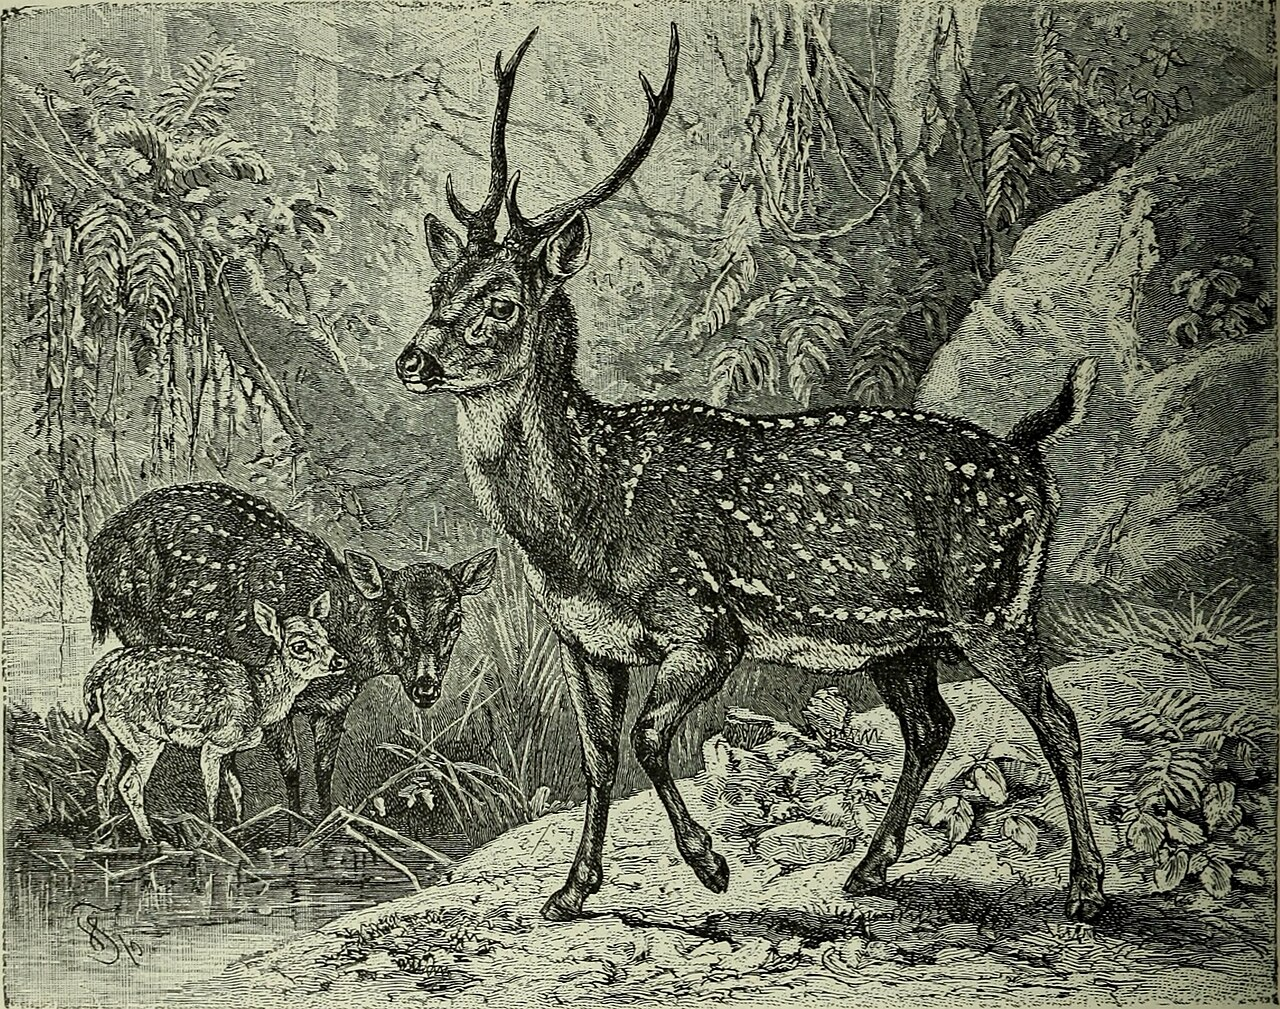
\includegraphics[width=12cm, height=4cm, keepaspectratio]{Billeder/Dyr/Pattedyr/hovdyr/hovdyr.jpg}\\[1.2em]
    {\LARGE \textbf{Hovdyr}}\\[0.6em]
    Klovbærende vildt\\[0.35em]
    Artsbestemmelse, vildtbiologi \& terminologi \\[0.9em]
    {\tiny\color{gray}
    CC BY 4.0 – kan frit anvendes, også kommercielt. Rettighederne må ikke skærpes.\\[0.05em]
    Udviklet af Aleksander Sønder, OSJAGTTEGN.DK}
  \end{center}
\end{frame}

% ========== KRONHJORT (KRONVILDT) ==========
\begin{frame}{%
  \begin{minipage}[c]{0.30\textwidth}
    Kronhjort
  \end{minipage}%
  \hfill
  \begin{minipage}[c]{0.45\textwidth}
    \footnotesize
    \textbf{Jagttid:} $\geq$ 10 sprosser: 16.\ okt.--31.\ dec.\\
    %Spids: 1.\ sep.--31.\ jan.\ \ Hind: 1.\ okt.--31.\ jan.\\
    %Kalv: 1.\ sep.--29.\ feb.*
  \end{minipage}%
  \hfill
  \begin{minipage}[c]{0.15\textwidth}
    \noindent\raggedleft
    
\includegraphics[width=0.5cm, height=0.5cm, keepaspectratio]{Billeder/Ikoner/star.png}%
    \hspace{0.2em}%
    
\includegraphics[width=0.5cm, height=0.5cm, keepaspectratio]{Billeder/Ikoner/star.png}%
    \hspace{0.2em}%
    
\includegraphics[width=0.5cm, height=0.5cm, keepaspectratio]{Billeder/Ikoner/star.png}
  \end{minipage}%
}
  \vspace{0.25em}
  \begin{columns}[T]
    % --- Venstre kolonne: Tekst ---
    \column{0.45\textwidth}
    \setlength{\parskip}{0.4em}
    \tiny
    \RaggedRight
    \textbf{\textit{Cervus elaphus}} – største hjorteart i Danmark. Hannen kaldes kronhjort og kendes på det store, forgrenede gevir. I andet leveår kaldes den kronspidshjort. \par
    \textbf{Udseende:}\\
    \quad – Langt snudeskaft \\
    \quad – Gult spejl der går op på ryggen \\
    \quad – Lange ører \par
    \textbf{Levesteder:} Store skovområder. Kræver meget ro. Nataktiv og opholder sig i tæt vegetation om dagen. \par
    \textbf{Føde:} Lyng, græs, lav, landbrugsafgrøder, skud fra buske/træer. \par
    \textbf{Udbredelse:} Jylland og Sjælland. \par
    \textbf{Parring/brunst:} September/oktober. \par
    \textbf{Forplantning:}\\
    \quad – \textbf{Kønsmoden:} 1 år \\
    \quad – \textbf{Mono/polygam:} Polygam \\
    \quad – \textbf{Bestandsomsætning:} Langsom \\
    %\quad – \textbf{Kuld:} 1 kalv, sjældent 2 \par
    %\textbf{*Bemærk:} Mange lokale jagttider.
    % --- Højre kolonne: Større billede ---
    \column{0.52\textwidth}
    \centering
    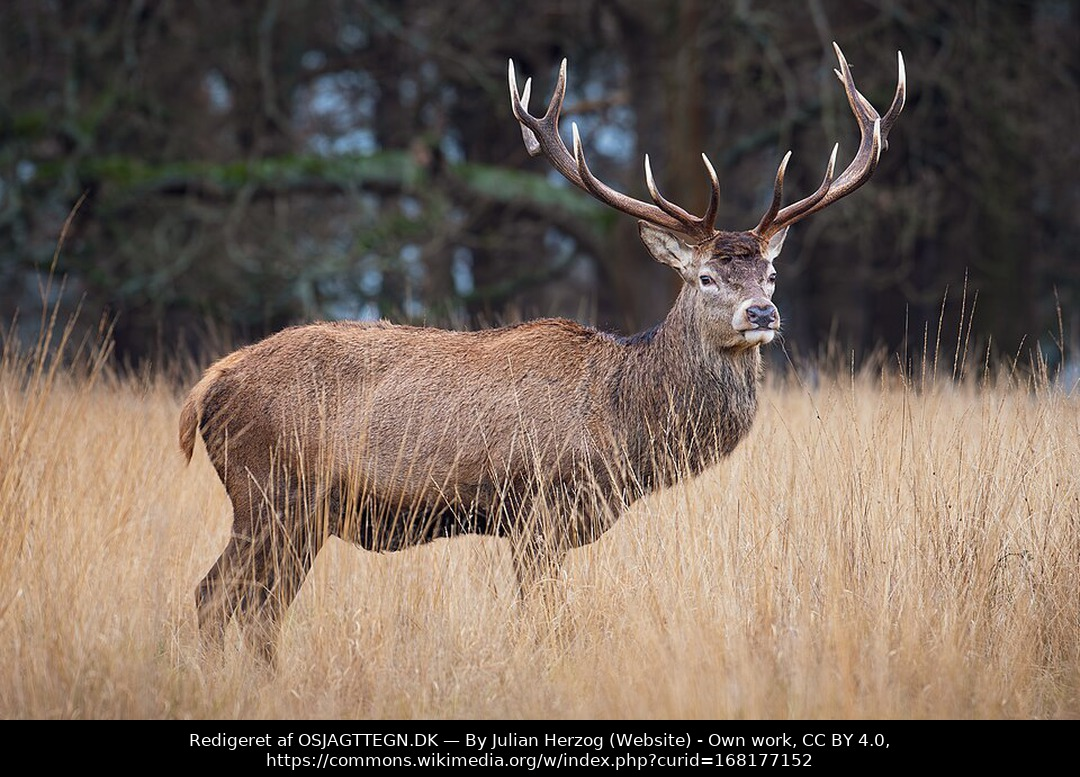
\includegraphics[width=\linewidth, height=7.2cm, keepaspectratio]{Billeder/Dyr/Pattedyr/hovdyr/kronvildt/kronhjort/kronvildt-male-03.jpg}
  \end{columns}
\end{frame}

% ========== KRONSPIDSHJORT ==========
\begin{frame}{%
  \begin{minipage}[c]{0.30\textwidth}
    Kronspidshjort
  \end{minipage}%
  \hfill
  \begin{minipage}[c]{0.45\textwidth}
    \footnotesize
    \textbf{Jagttid:} 1.\ september -- 31.\ januar
  \end{minipage}%
  \hfill
  \begin{minipage}[c]{0.15\textwidth}
    \noindent\raggedleft
    
\includegraphics[width=0.5cm, height=0.5cm, keepaspectratio]{Billeder/Ikoner/star.png}%
    \hspace{0.2em}%
    
\includegraphics[width=0.5cm, height=0.5cm, keepaspectratio]{Billeder/Ikoner/star.png}%
    \hspace{0.2em}%
    
\includegraphics[width=0.5cm, height=0.5cm, keepaspectratio]{Billeder/Ikoner/star.png}
  \end{minipage}%
}
  \vspace{0.25em}
  \begin{columns}[T]
    % --- Venstre kolonne: Tekst ---
    \column{0.45\textwidth}
    \setlength{\parskip}{0.4em}
    \tiny
    \RaggedRight
    \textbf{\textit{Cervus elaphus}} – kronhjort i sit andet leveår. Kaldes spidshjort, fordi geviret typisk kun består af to enkelte spidser. \par
    \textbf{Udseende:}\\
    \quad – To enkle gevirstænger uden forgrening \\
    \quad – Mindre og slankere end ældre hjort \\
    \quad – Gult spejl der går op på ryggen \par
    \textbf{Levesteder:} Store skovområder. Kræver meget ro. Nataktiv og opholder sig i tæt vegetation om dagen. \par
    \textbf{Føde:} Lyng, græs, lav, landbrugsafgrøder, skud fra buske/træer. \par
    \textbf{Udbredelse:} Jylland og Sjælland. \par
    \textbf{Parring/brunst:} September/oktober. \par
    %\textbf{Forplantning:}\\
    %\quad – \textbf{Kønsmoden:} 1 år \\
    %\quad – \textbf{Mono/polygam:} Polygam \\
    %\quad – \textbf{Bestandsomsætning:} Langsom \\
    %\quad – \textbf{Kuld:} 1 kalv, sjældent 2 \par
    %\textbf{*Bemærk:} Mange lokale jagttider.
    % --- Højre kolonne: Større billede ---
    \column{0.52\textwidth}
    \centering
    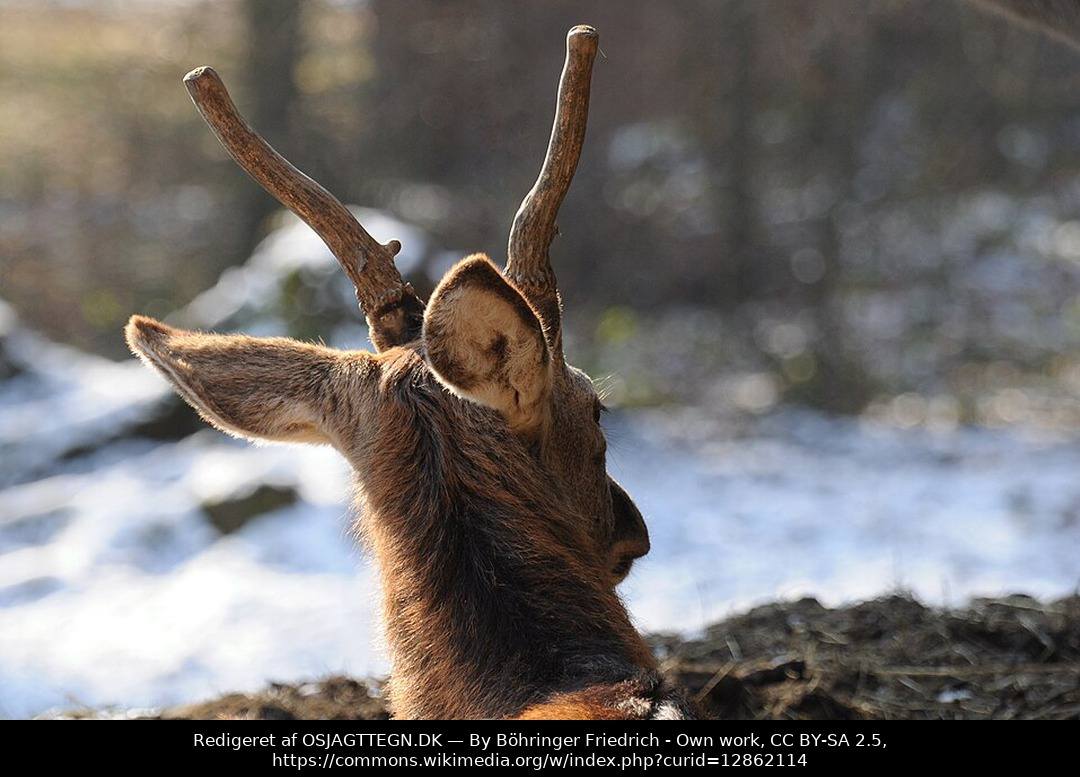
\includegraphics[width=\linewidth, height=7.2cm, keepaspectratio]{Billeder/Dyr/Pattedyr/hovdyr/kronvildt/kronspidshjort/kronspidshjort-01.JPG}
  \end{columns}
\end{frame}

% ========== KRONHIND ==========
\begin{frame}{%
  \begin{minipage}[c]{0.30\textwidth}
    Kronhind
  \end{minipage}%
  \hfill
  \begin{minipage}[c]{0.45\textwidth}
    \footnotesize
    \textbf{Jagttid:} 1.\ oktober -- 31.\ januar
  \end{minipage}%
  \hfill
  \begin{minipage}[c]{0.15\textwidth}
    \noindent\raggedleft
    
\includegraphics[width=0.5cm, height=0.5cm, keepaspectratio]{Billeder/Ikoner/star.png}%
    \hspace{0.2em}%
    
\includegraphics[width=0.5cm, height=0.5cm, keepaspectratio]{Billeder/Ikoner/star.png}%
    \hspace{0.2em}%
    
\includegraphics[width=0.5cm, height=0.5cm, keepaspectratio]{Billeder/Ikoner/star.png}
  \end{minipage}%
}
  \vspace{0.25em}
  \begin{columns}[T]
    \column{0.45\textwidth}
    \setlength{\parskip}{0.4em}
    \tiny
    \RaggedRight
    \textbf{\textit{Cervus elaphus}} – hunnen hos kronvildt. I andet leveår kaldes den smalhind, hvis den endnu ikke har fået kalv. Lever ofte i familiegruppe med kalv og andre hinder. \par
    \textbf{Udseende:}\\
    \quad – Intet gevir \\
    \quad – Langt snudeskaft \\
    \quad – Gult spejl der går op på ryggen \\
    \quad – Lange ører \par
    \textbf{Levesteder:} Store skovområder. Kræver meget ro. Nataktiv og opholder sig i tæt vegetation om dagen. \par
    \textbf{Føde:} Lyng, græs, lav, landbrugsafgrøder, skud fra buske/træer. \par
    %\textbf{Udbredelse:} Jylland og Sjælland. \par
    %\textbf{Parring/brunst:} September/oktober. \par
    \textbf{Forplantning:}\\
    \quad – \textbf{Kønsmoden:} 1 år \\
    \quad – \textbf{Mono/polygam:} Polygam \\
    \quad – \textbf{Bestandsomsætning:} Langsom \\
    \quad – \textbf{Kuld:} 1 kalv, sjældent 2 \par
    %\textbf{*Bemærk:} Mange lokale jagttider.
    \column{0.52\textwidth}
    \centering
    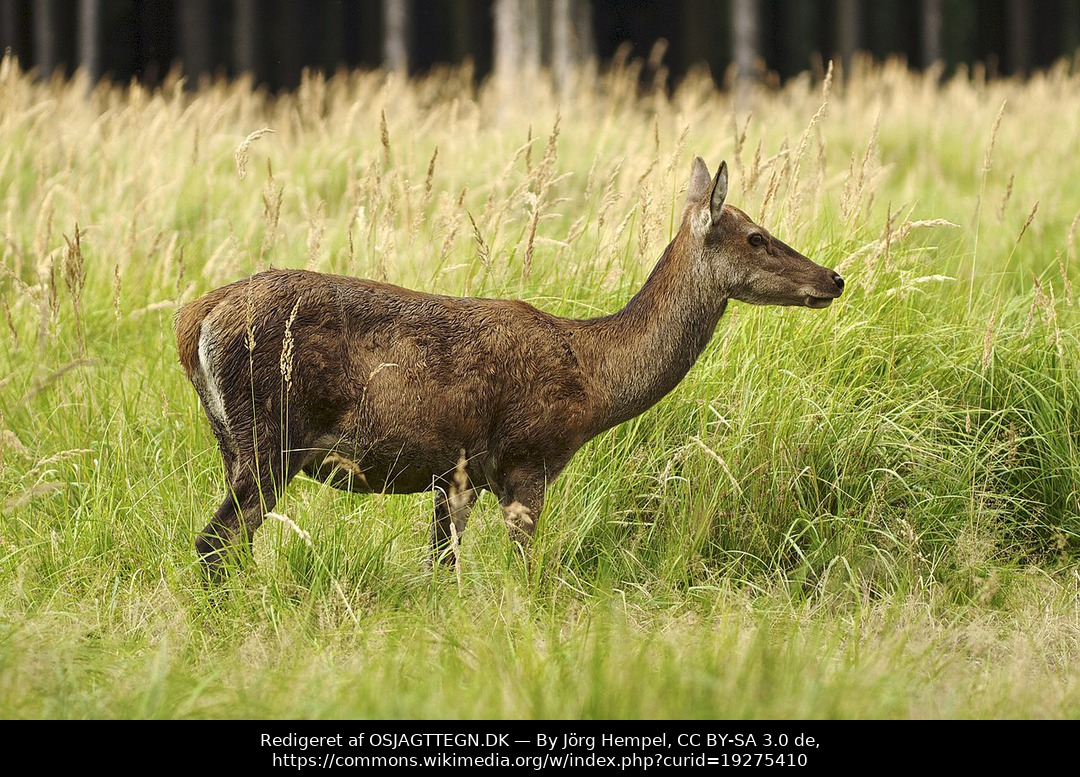
\includegraphics[width=\linewidth, height=7.2cm, keepaspectratio]{Billeder/Dyr/Pattedyr/hovdyr/kronvildt/kronhind/kronvildt-female-01.jpg}
  \end{columns}
\end{frame}

% ========== KRONKALV ==========
\begin{frame}{%
  \begin{minipage}[c]{0.30\textwidth}
    Kronkalv
  \end{minipage}%
  \hfill
  \begin{minipage}[c]{0.45\textwidth}
    \footnotesize
    \textbf{Jagttid:} 1.\ september -- 29.\ februar
  \end{minipage}%
  \hfill
  \begin{minipage}[c]{0.15\textwidth}
    \noindent\raggedleft
    
\includegraphics[width=0.5cm, height=0.5cm, keepaspectratio]{Billeder/Ikoner/star.png}%
    \hspace{0.2em}%
    
\includegraphics[width=0.5cm, height=0.5cm, keepaspectratio]{Billeder/Ikoner/star.png}%
    \hspace{0.2em}%
    
\includegraphics[width=0.5cm, height=0.5cm, keepaspectratio]{Billeder/Ikoner/star.png}
  \end{minipage}%
}
  \vspace{0.25em}
  \begin{columns}[T]
    \column{0.45\textwidth}
    \setlength{\parskip}{0.4em}
    \tiny
    \RaggedRight
    \textbf{\textit{Cervus elaphus}} – unge af kronvildt i sit første leveår. Lever typisk sammen med hinder og smalhinder i en familiegruppe eller rudel. \par
    \textbf{Udseende:}\\
    \quad – Mindre end hind og hjort \\
    \quad – Kortere hals og snudeskaft \\
    \quad – Intet gevir \\
    \quad – Gult spejl der går op på ryggen \\
    \quad – Kan have lyse pletter som helt lille \par
    %\textbf{Levesteder:} Store skovområder. Kræver meget ro. Nataktiv og opholder sig i tæt vegetation om dagen. \par
    %\textbf{Føde:} Lyng, græs, lav, landbrugsafgrøder, skud fra buske/træer. \par
    %\textbf{Udbredelse:} Jylland og Sjælland. \par
    %\textbf{Parring/brunst:} Født efter brunst i september/oktober. \par
    %\textbf{Forplantning:}\\
    %\quad – \textbf{Kønsmoden:} 1 år \\
    %\quad – \textbf{Mono/polygam:} Polygam \\
    %\quad – \textbf{Bestandsomsætning:} Langsom \\
    %\quad – \textbf{Kuld:} 1 kalv, sjældent 2 \par
    %\textbf{*Bemærk:} Mange lokale jagttider.
    \column{0.52\textwidth}
    \centering
    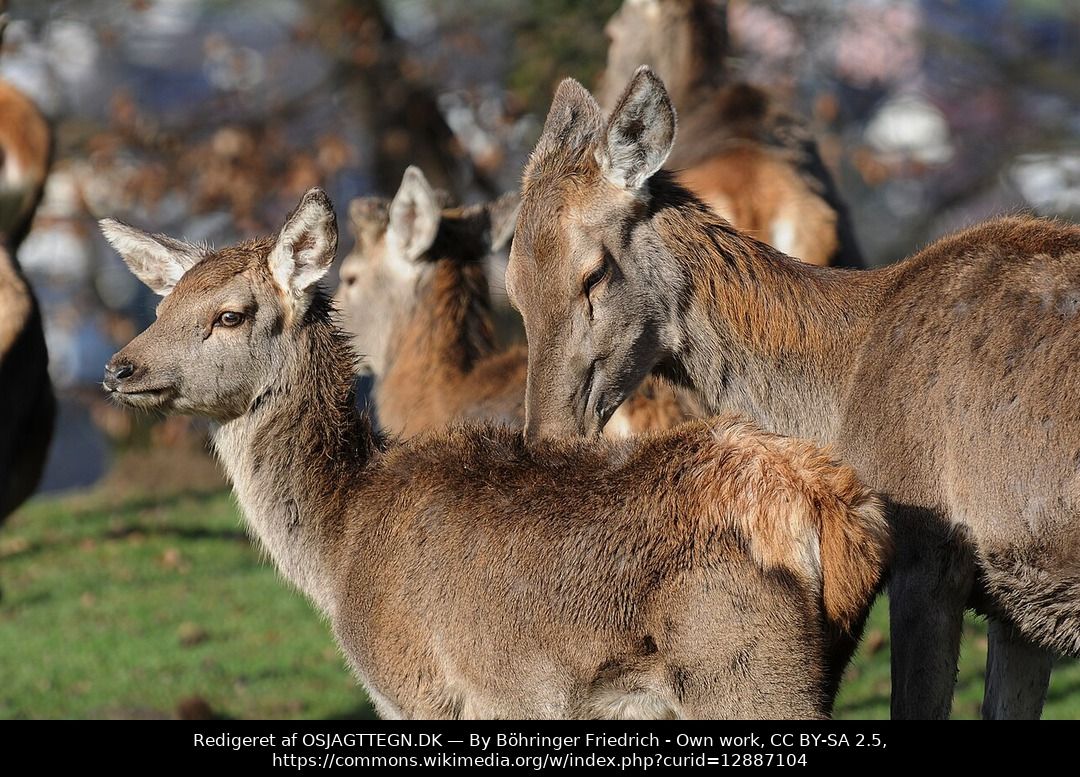
\includegraphics[width=\linewidth, height=7.2cm, keepaspectratio]{Billeder/Dyr/Pattedyr/hovdyr/kronvildt/kronkalv/kronvildt-female-05.jpeg}
  \end{columns}
\end{frame}

% ========== DÅHJORT ==========
\begin{frame}{%
  \begin{minipage}[c]{0.30\textwidth}
    Dåhjort
  \end{minipage}%
  \hfill
  \begin{minipage}[c]{0.45\textwidth}
    \footnotesize
    \textbf{Jagttid:} 1.\ september -- 31.\ januar
  \end{minipage}%
  \hfill
  \begin{minipage}[c]{0.15\textwidth}
    \noindent\raggedleft
    
\includegraphics[width=0.5cm, height=0.5cm, keepaspectratio]{Billeder/Ikoner/star.png}%
    \hspace{0.2em}%
    
\includegraphics[width=0.5cm, height=0.5cm, keepaspectratio]{Billeder/Ikoner/star.png}%
    \hspace{0.2em}%
    
\includegraphics[width=0.5cm, height=0.5cm, keepaspectratio]{Billeder/Ikoner/star.png}
  \end{minipage}%
}
  \vspace{0.25em}
  \begin{columns}[T]
    \column{0.45\textwidth}
    \setlength{\parskip}{0.4em}
    \tiny
    \RaggedRight
    \textbf{\textit{Dama dama}} – næststørste hjorteart i Danmark. Hannen kaldes dåhjort og kendes på det skovlede (plade) gevir. I andet leveår kaldes den dåspidshjort. \par
    \textbf{Udseende:}\\
    \quad – Kort snudeskaft \\
    \quad – Hvidt spejl (111) \\
    \quad – Mange farvevariationer med pletter \par
    \textbf{Levesteder:} Skov, hegn og åbne landskaber. \par
    \textbf{Føde:} Græsser, urter, olden og landbrugsafgrøder. \par
    \textbf{Udbredelse:} Hele landet. \par
    \textbf{Parring/brunst:} Oktober/november. \par
    \textbf{Forplantning:}\\
    \quad – \textbf{Kønsmoden:} 1 år \\
    \quad – \textbf{Mono/polygam:} Polygam \\
    \quad – \textbf{Bestandsomsætning:} Langsom \\
    \quad – \textbf{Kuld:} 1 kalv, sjældent 2 \par
    %\textbf{*Bemærk:} Mange lokale jagttider.
    \column{0.52\textwidth}
    \centering
    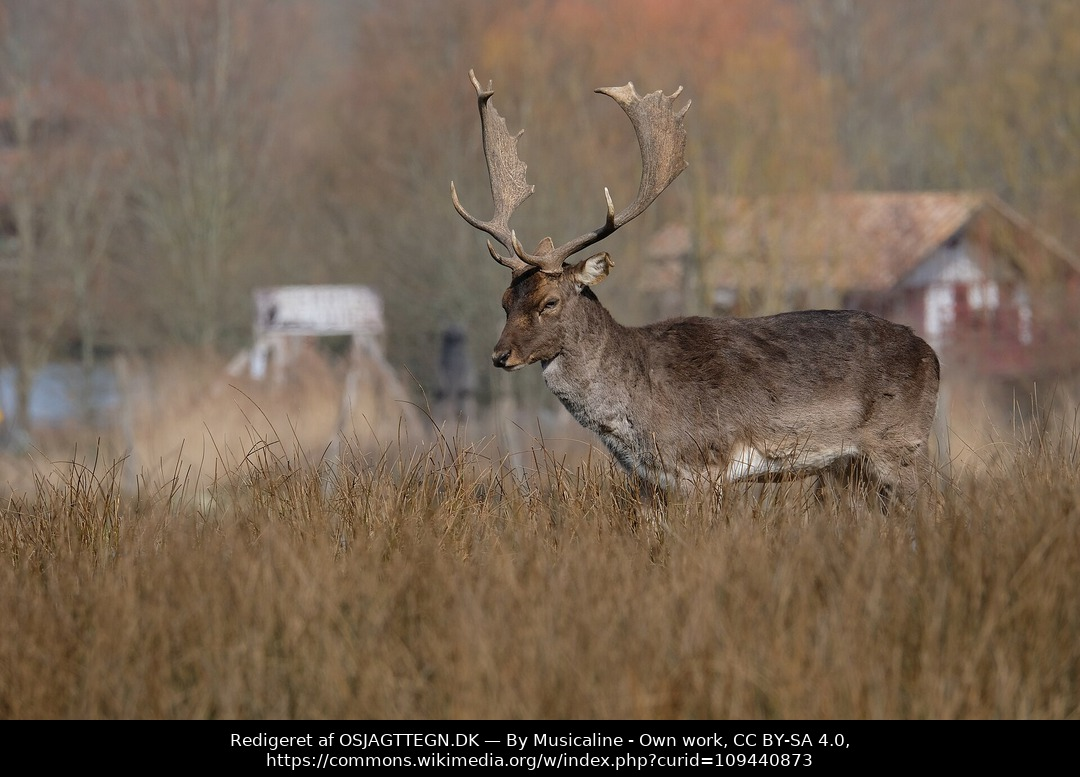
\includegraphics[width=\linewidth, height=7.2cm, keepaspectratio]{Billeder/Dyr/Pattedyr/hovdyr/dåvildt/daavildt-male-05.jpg}
  \end{columns}
\end{frame}

% ========== DÅSPIDSHJORT ==========
\begin{frame}{%
  \begin{minipage}[c]{0.30\textwidth}
    Dåspidshjort
  \end{minipage}%
  \hfill
  \begin{minipage}[c]{0.45\textwidth}
    \footnotesize
    \textbf{Jagttid:} 1.\ september -- 31.\ januar
  \end{minipage}%
  \hfill
  \begin{minipage}[c]{0.15\textwidth}
    \noindent\raggedleft
    
\includegraphics[width=0.5cm, height=0.5cm, keepaspectratio]{Billeder/Ikoner/star.png}%
    \hspace{0.2em}%
    
\includegraphics[width=0.5cm, height=0.5cm, keepaspectratio]{Billeder/Ikoner/star.png}%
    \hspace{0.2em}%
    
\includegraphics[width=0.5cm, height=0.5cm, keepaspectratio]{Billeder/Ikoner/star.png}
  \end{minipage}%
}
  \vspace{0.25em}
  \begin{columns}[T]
    \column{0.45\textwidth}
    \setlength{\parskip}{0.4em}
    \tiny
    \RaggedRight
    \textbf{\textit{Dama dama}} – dåhjort i sit andet leveår. Kaldes dåspidshjort, fordi geviret typisk kun består af to enkelte spidser. \par
    \textbf{Udseende:}\\
    \quad – To enkle gevirstænger uden skovle \\
    \quad – Kort snudeskaft \\
    \quad – Hvidt spejl (111) \\
    \quad – Mindre og slankere end ældre dåhjort \par
    \textbf{Levesteder:} Skov, hegn og åbne landskaber. \par
    \textbf{Føde:} Græsser, urter, olden og landbrugsafgrøder. \par
    \textbf{Udbredelse:} Hele landet. \par
    \textbf{Parring/brunst:} Oktober/november. \par
    \textbf{Forplantning:}\\
    \quad – \textbf{Kønsmoden:} 1 år \\
    \quad – \textbf{Mono/polygam:} Polygam \\
    \quad – \textbf{Bestandsomsætning:} Langsom \\
    \quad – \textbf{Kuld:} 1 kalv, sjældent 2 \par
    %\textbf{*Bemærk:} Mange lokale jagttider.
    \column{0.52\textwidth}
    \centering
    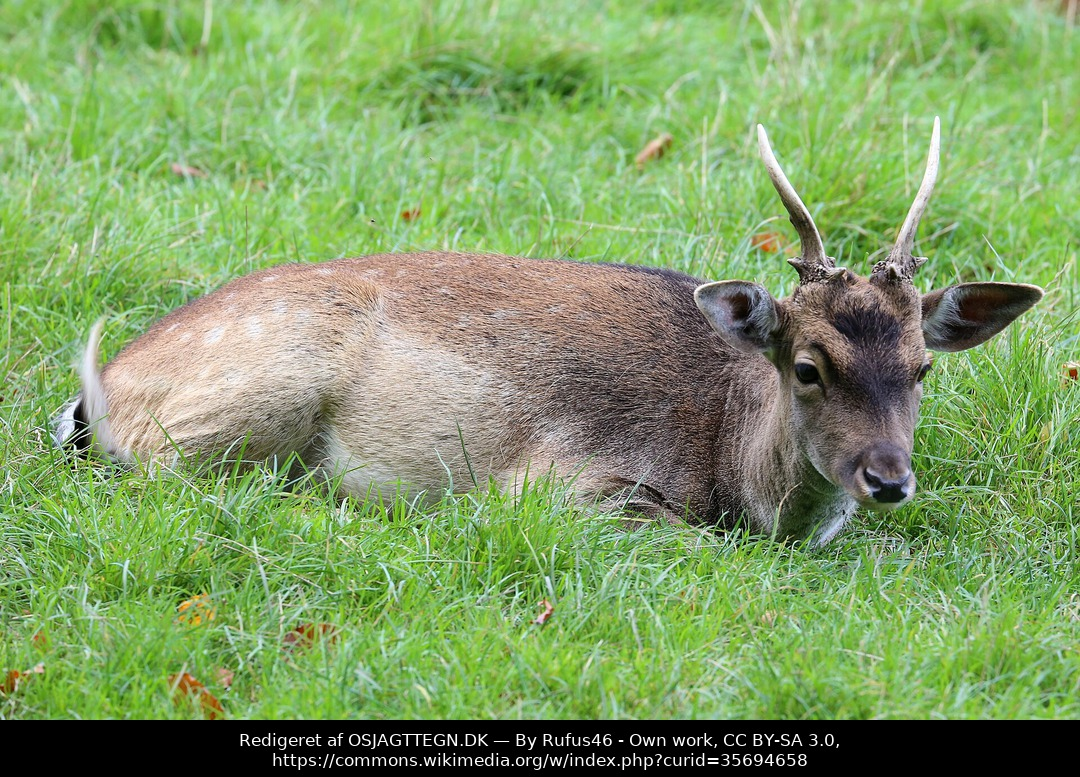
\includegraphics[width=\linewidth, height=7.2cm, keepaspectratio]{Billeder/Dyr/Pattedyr/hovdyr/dåvildt/dåspidshjort/daavildt-spidshjort-02.jpg}
  \end{columns}
\end{frame}

% ========== DÅ ==========
\begin{frame}{%
  \begin{minipage}[c]{0.30\textwidth}
    Då
  \end{minipage}%
  \hfill
  \begin{minipage}[c]{0.45\textwidth}
    \footnotesize
    \textbf{Jagttid:} 1.\ oktober -- 31.\ januar
  \end{minipage}%
  \hfill
  \begin{minipage}[c]{0.15\textwidth}
    \noindent\raggedleft
    
\includegraphics[width=0.5cm, height=0.5cm, keepaspectratio]{Billeder/Ikoner/star.png}%
    \hspace{0.2em}%
    
\includegraphics[width=0.5cm, height=0.5cm, keepaspectratio]{Billeder/Ikoner/star.png}%
    \hspace{0.2em}%
    
\includegraphics[width=0.5cm, height=0.5cm, keepaspectratio]{Billeder/Ikoner/star.png}
  \end{minipage}%
}
  \vspace{0.25em}
  \begin{columns}[T]
    \column{0.45\textwidth}
    \setlength{\parskip}{0.4em}
    \tiny
    \RaggedRight
    \textbf{\textit{Dama dama}} – hunnen hos dåvildt. I andet leveår kaldes den smaldå, hvis den endnu ikke har fået kalv. Då, smaldå og dåkalv lever ofte i familiegruppe. Flere dåer med afkom kaldes en rudel. \par
    \textbf{Udseende:}\\
    \quad – Intet gevir \\
    \quad – Kort snudeskaft \\
    \quad – Hvidt spejl (111) \\
    \quad – Mange farvevariationer med pletter \par
    \textbf{Levesteder:} Skov, hegn og åbne landskaber. \par
    \textbf{Føde:} Græsser, urter, olden og landbrugsafgrøder. \par
    \textbf{Udbredelse:} Hele landet. \par
    \textbf{Parring/brunst:} Oktober/november. \par
    \textbf{Forplantning:}\\
    \quad – \textbf{Kønsmoden:} 1 år \\
    \quad – \textbf{Mono/polygam:} Polygam \\
    \quad – \textbf{Bestandsomsætning:} Langsom \\
    \quad – \textbf{Kuld:} 1 kalv, sjældent 2 \par
    %\textbf{*Bemærk:} Mange lokale jagttider.
    \column{0.52\textwidth}
    \centering
    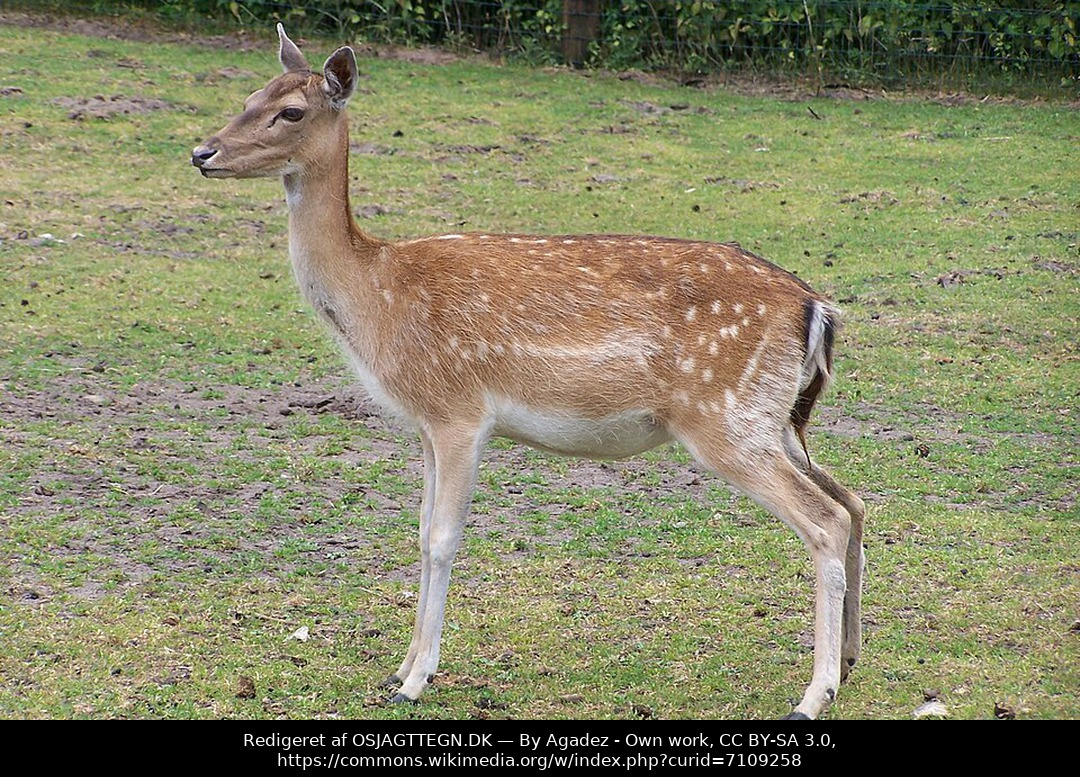
\includegraphics[width=\linewidth, height=7.2cm, keepaspectratio]{Billeder/Dyr/Pattedyr/hovdyr/dåvildt/daavildt-female-02.jpg}
  \end{columns}
\end{frame}

% ========== DÅKALV ==========
\begin{frame}{%
  \begin{minipage}[c]{0.30\textwidth}
    Dåkalv
  \end{minipage}%
  \hfill
  \begin{minipage}[c]{0.45\textwidth}
    \footnotesize
    \textbf{Jagttid:} 1.\ oktober -- 31.\ januar
  \end{minipage}%
  \hfill
  \begin{minipage}[c]{0.15\textwidth}
    \noindent\raggedleft
    
\includegraphics[width=0.5cm, height=0.5cm, keepaspectratio]{Billeder/Ikoner/star.png}%
    \hspace{0.2em}%
    
\includegraphics[width=0.5cm, height=0.5cm, keepaspectratio]{Billeder/Ikoner/star.png}%
    \hspace{0.2em}%
    
\includegraphics[width=0.5cm, height=0.5cm, keepaspectratio]{Billeder/Ikoner/star.png}
  \end{minipage}%
}
  \vspace{0.25em}
  \begin{columns}[T]
    \column{0.45\textwidth}
    \setlength{\parskip}{0.4em}
    \tiny
    \RaggedRight
    \textbf{\textit{Dama dama}} – unge af dåvildt i sit første leveår. Lever typisk sammen med dåen. \par
    \textbf{Udseende:}\\
    \quad – Mindre end då og dåhjort \\
    \quad – Intet gevir \\
    \quad – Hvidt spejl (111) \\
    \quad – Ofte tydeligt plettet, især som helt lille \par
    \textbf{Levesteder:} Skov, hegn og åbne landskaber. \par
    \textbf{Føde:} Græsser, urter, olden og landbrugsafgrøder. \par
    \textbf{Udbredelse:} Hele landet. \par
    \textbf{Parring/brunst:} Født efter brunst i oktober/november. \par
    \textbf{Forplantning:}\\
    \quad – \textbf{Kønsmoden:} 1 år \\
    \quad – \textbf{Mono/polygam:} Polygam \\
    \quad – \textbf{Bestandsomsætning:} Langsom \\
    \quad – \textbf{Kuld:} 1 kalv, sjældent 2 \par
    \column{0.52\textwidth}
    \centering
    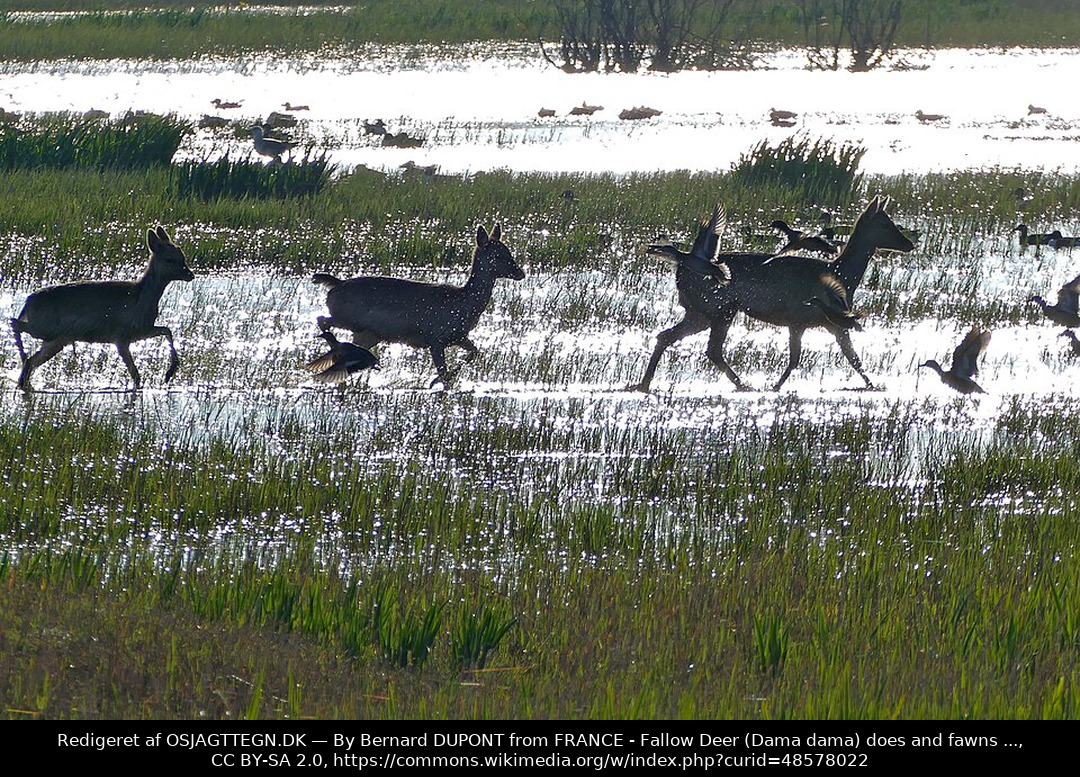
\includegraphics[width=\linewidth, height=7.2cm, keepaspectratio]{Billeder/Dyr/Pattedyr/hovdyr/dåvildt/daavildt-kalv-01.jpg}
  \end{columns}
\end{frame}

% ========== RÅBUK ==========
\begin{frame}{%
  \begin{minipage}[c]{0.30\textwidth}
    Råbuk
  \end{minipage}%
  \hfill
  \begin{minipage}[c]{0.45\textwidth}
    \footnotesize
    \textbf{Jagttid:} 16.\ maj -- 15.\ jul.\\
    samt 1.\ okt.--31.\ jan.
  \end{minipage}%
  \hfill
  \begin{minipage}[c]{0.15\textwidth}
    \noindent\raggedleft
    
\includegraphics[width=0.5cm, height=0.5cm, keepaspectratio]{Billeder/Ikoner/star.png}%
    \hspace{0.2em}%
    
\includegraphics[width=0.5cm, height=0.5cm, keepaspectratio]{Billeder/Ikoner/star.png}%
    \hspace{0.2em}%
    
\includegraphics[width=0.5cm, height=0.5cm, keepaspectratio]{Billeder/Ikoner/star.png}
  \end{minipage}%
}
  \vspace{0.25em}
  \begin{columns}[T]
    \column{0.45\textwidth}
    \setlength{\parskip}{0.4em}
    \tiny
    \RaggedRight
    \textbf{\textit{Capreolus capreolus}} – mindste hjorteart i Danmark. Hannen kaldes råbuk og kendes på det lille gevir. I andet leveår kaldes den spidsbuk. \par
    \textbf{Udseende:}\\
    \quad – Kort snudeskaft med sort plet \\
    \quad – Gulligt/hvidt spejl \\
    \quad – Rødbrun/grå \par
    \textbf{Levesteder:} Randzoner og nye skovarealer. Mest aktiv morgen og aften. \par
    \textbf{Føde:} Græsser, urter, knopper og skud fra buske. \par
    \textbf{Udbredelse:} Hele landet. \par
    \textbf{Yngleforhold:} Forlænget drægtighed. \par
    \textbf{Parring/brunst:} Slutningen af juli / starten af august. \par
    \textbf{Sygdomme:} Svælgbremser, pelslus
    \textbf{Forplantning:}\\
    \quad – \textbf{Kønsmoden:} 1 år \\
    \quad – \textbf{Mono/polygam:} Polygam \\
    \quad – \textbf{Bestandsomsætning:} Hurtig \\
    \quad – \textbf{Kuld:} 1--3 lam, oftest 2 \par
    %\textbf{*Bemærk:} Lokale jagttider kan forekomme.
    \column{0.52\textwidth}
    \centering
    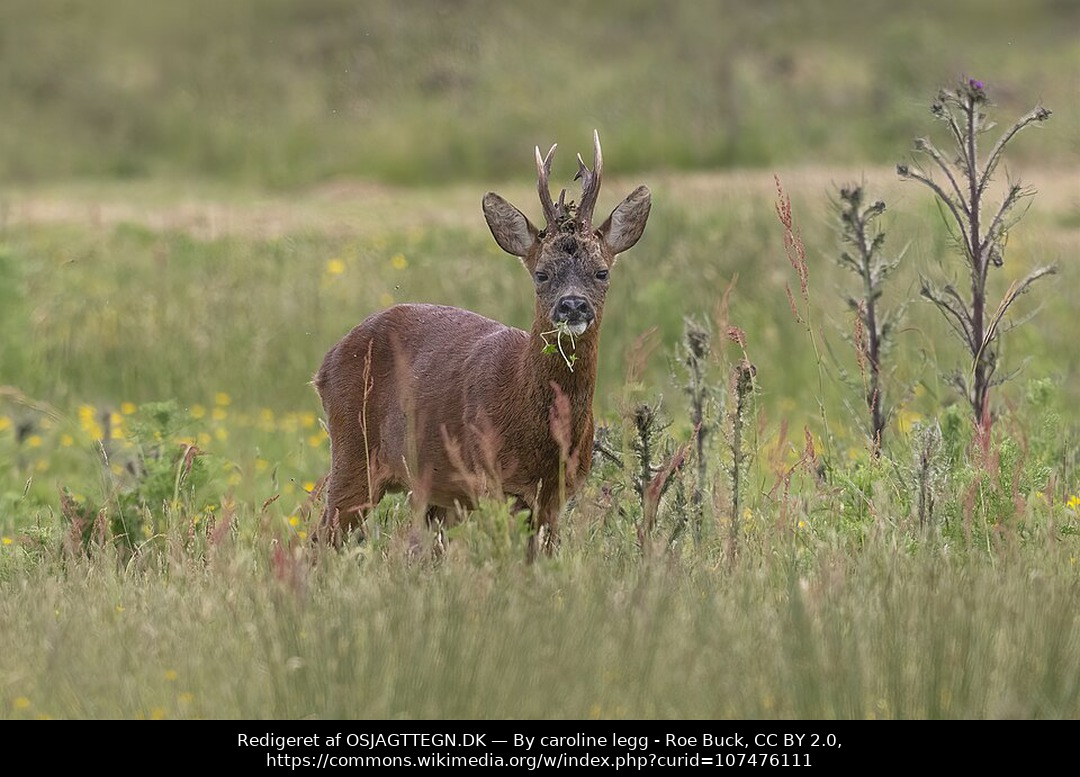
\includegraphics[width=\linewidth, height=7.2cm, keepaspectratio]{Billeder/Dyr/Pattedyr/hovdyr/råvildt/raavildt-male-10.jpg}
  \end{columns}
\end{frame}

% ========== RÅ OG RÅLAM ==========
\begin{frame}{%
  \begin{minipage}[c]{0.30\textwidth}
    Rå og rålam
  \end{minipage}%
  \hfill
  \begin{minipage}[c]{0.45\textwidth}
    \footnotesize
    \textbf{Jagttid:} 1.\ oktober -- 31.\ januar*
  \end{minipage}%
  \hfill
  \begin{minipage}[c]{0.15\textwidth}
    \noindent\raggedleft
    
\includegraphics[width=0.5cm, height=0.5cm, keepaspectratio]{Billeder/Ikoner/star.png}%
    \hspace{0.2em}%
    
\includegraphics[width=0.5cm, height=0.5cm, keepaspectratio]{Billeder/Ikoner/star.png}%
    \hspace{0.2em}%
    
\includegraphics[width=0.5cm, height=0.5cm, keepaspectratio]{Billeder/Ikoner/star.png}
  \end{minipage}%
}
  \vspace{0.25em}
  \begin{columns}[T]
    \column{0.45\textwidth}
    \setlength{\parskip}{0.4em}
    \tiny
    \RaggedRight
    \textbf{\textit{Capreolus capreolus}} – hunnen kaldes rå. En rå der har sat lam kaldes gammelrå. I andet leveår kaldes den smalrå. Ungen kaldes bukkelam eller rålam afhængigt af køn. \par
    \textbf{Udseende:}\\
    \quad – Kort snudeskaft med sort plet \\
    \quad – Gulligt/hvidt spejl \\
    \quad – Rødbrun/grå \par
    \textbf{Levesteder:} Randzoner og nye skovarealer. Mest aktiv morgen og aften. \par
    \textbf{Føde:} Græsser, urter, knopper og skud fra buske. \par
    \textbf{Udbredelse:} Hele landet. \par
    \textbf{Yngleforhold:} Forlænget drægtighed. \par
    \textbf{Parring/brunst:} Slutningen af juli / starten af august. \par
    \textbf{Forplantning:}\\
    \quad – \textbf{Kønsmoden:} 1 år \\
    \quad – \textbf{Mono/polygam:} Polygam \\
    \quad – \textbf{Bestandsomsætning:} Hurtig \\
    \quad – \textbf{Kuld:} 1--3 lam \par
    \textbf{*Bemærk:} Lokale jagttider kan forekomme.
    \column{0.52\textwidth}
    \centering
    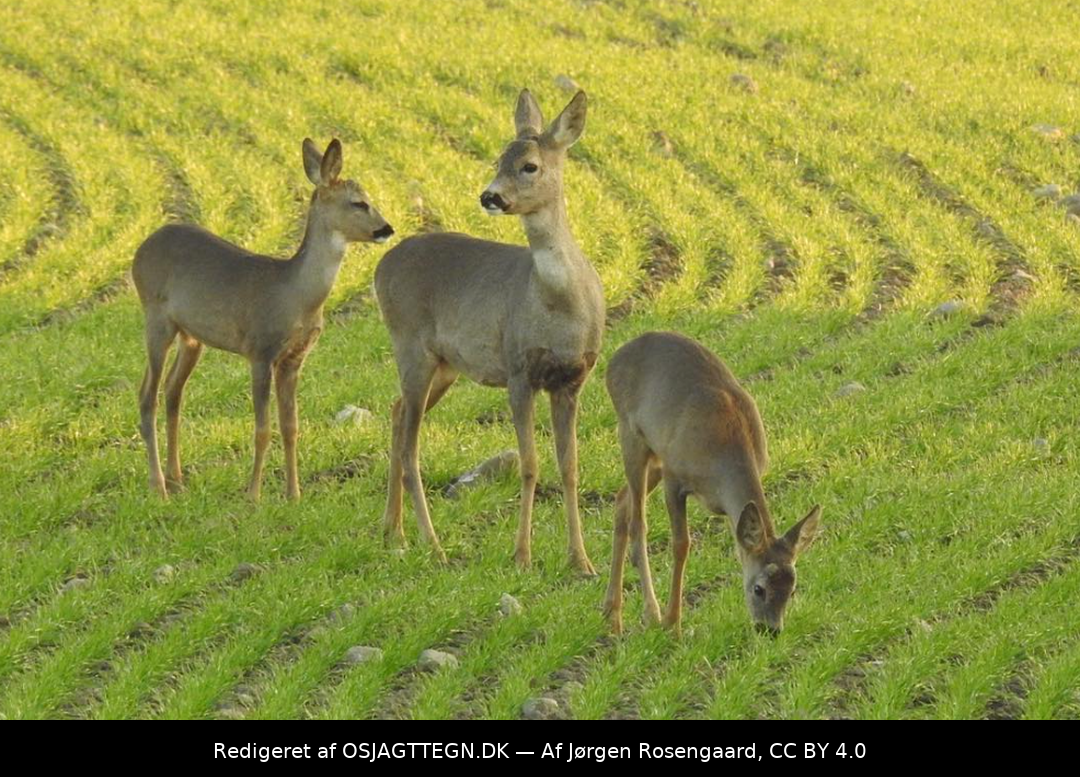
\includegraphics[width=\linewidth, height=7.2cm, keepaspectratio]{Billeder/Dyr/Pattedyr/hovdyr/råvildt/raavildt-family-01.png}
  \end{columns}
\end{frame}

% ========== SIKAHJORT ==========
\begin{frame}{%
  \begin{minipage}[c]{0.30\textwidth}
    Sikahjort
  \end{minipage}%
  \hfill
  \begin{minipage}[c]{0.45\textwidth}
    \footnotesize
    \textbf{Jagttid:} 1.\ september -- 31.\ januar
  \end{minipage}%
  \hfill
  \begin{minipage}[c]{0.15\textwidth}
    \noindent\raggedleft
    
\includegraphics[width=0.5cm, height=0.5cm, keepaspectratio]{Billeder/Ikoner/star.png}
  \end{minipage}%
}
  \vspace{0.25em}
  \begin{columns}[T]
    \column{0.45\textwidth}
    \setlength{\parskip}{0.4em}
    \tiny
    \RaggedRight
    \textbf{\textit{Cervus nippon}} – mindre hjorteart end kron- og dåvildt. Hannen kaldes sikahjort. \par
    \textbf{Udseende:}\\
    \quad – Hvidt spejl, men de sorte aftegninger fortsætter ned på bagbenene \\
    \quad – Ansigtsudtryk som med løftede øjenbryn \\
    \quad – Gevir uden skovle, typisk slankere end dåhjort \par
    \textbf{Levesteder:} Skov og skovbryn, især med tæt underskov. \par
    \textbf{Føde:} Græs, urter, skud og landbrugsafgrøder. \par
    \textbf{Udbredelse:} Især Djursland, men også andre steder i Danmark. \par
    \textbf{Parring/brunst:} Oktober. \par
    \textbf{Forplantning:}\\
    \quad – \textbf{Kønsmoden:} 1--2 år \\
    \quad – \textbf{Mono/polygam:} Polygam \\
    \quad – \textbf{Bestandsomsætning:} Langsom \\
    \quad – \textbf{Kuld:} 1 kalv
    \column{0.52\textwidth}
    \centering
    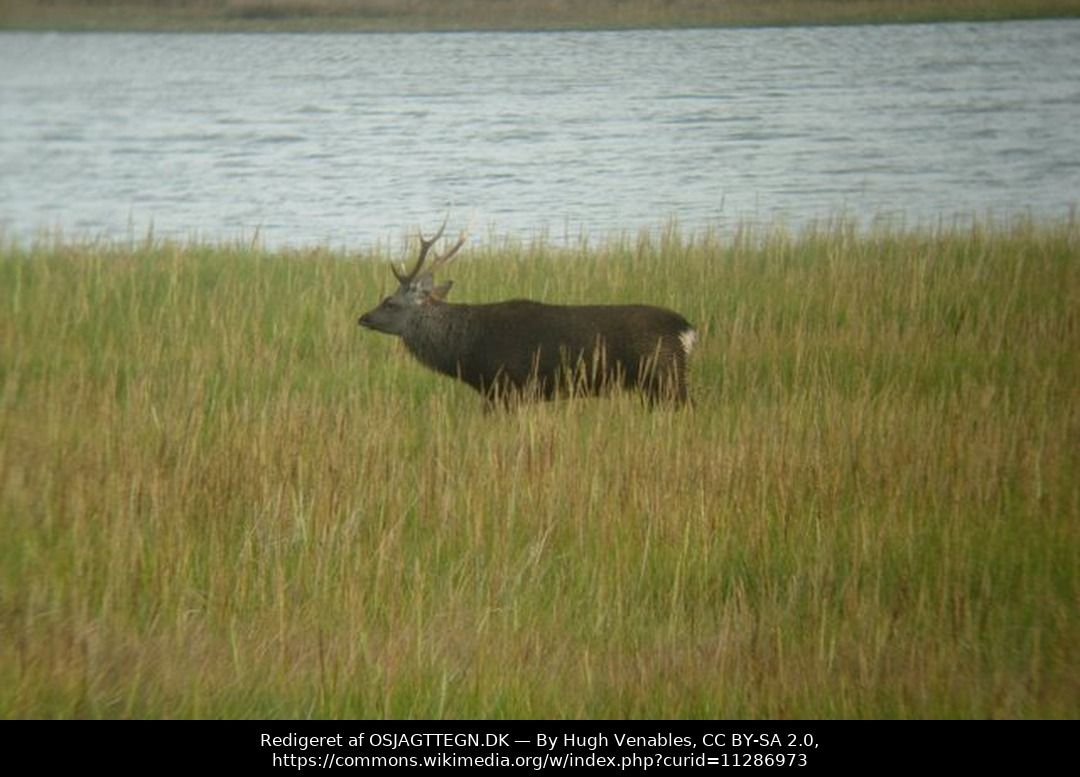
\includegraphics[width=\linewidth, height=7.2cm, keepaspectratio]{Billeder/Dyr/Pattedyr/hovdyr/sikavildt/sikavildt-male-06.jpg}
  \end{columns}
\end{frame}

% ========== SIKAHIND OG SIKAKALV ==========
\begin{frame}{%
  \begin{minipage}[c]{0.30\textwidth}
    Sikahind og sikakalv
  \end{minipage}%
  \hfill
  \begin{minipage}[c]{0.45\textwidth}
    \footnotesize
    \textbf{Jagttid:} 1.\ oktober -- 31.\ januar
  \end{minipage}%
  \hfill
  \begin{minipage}[c]{0.15\textwidth}
    \noindent\raggedleft
    
\includegraphics[width=0.5cm, height=0.5cm, keepaspectratio]{Billeder/Ikoner/star.png}
  \end{minipage}%
}
  \vspace{0.25em}
  \begin{columns}[T]
    \column{0.45\textwidth}
    \setlength{\parskip}{0.4em}
    \tiny
    \RaggedRight
    \textbf{\textit{Cervus nippon}} – hunnen kaldes sikahind. Ungen i første leveår kaldes sikakalv. Lever ofte sammen i mindre familiegrupper. \par
    \textbf{Udseende:}\\
    \quad – Intet gevir \\
    \quad – Hvidt spejl, hvor de sorte aftegninger fortsætter ned på bagbenene \\
    \quad – Ansigtsudtryk som med løftede øjenbryn \\
    \quad – Kalven er mindre og ofte tydeligere plettet \par
    \textbf{Levesteder:} Skov og skovbryn, især med tæt underskov. \par
    \textbf{Føde:} Græs, urter, skud og landbrugsafgrøder. \par
    \textbf{Udbredelse:} Især Djursland, men også andre steder i Danmark. \par
    \textbf{Parring/brunst:} Oktober. \par
    \textbf{Forplantning:}\\
    \quad – \textbf{Kønsmoden:} 1--2 år \\
    \quad – \textbf{Mono/polygam:} Polygam \\
    \quad – \textbf{Bestandsomsætning:} Langsom \\
    \quad – \textbf{Kuld:} 1 kalv
    \column{0.52\textwidth}
    \centering
    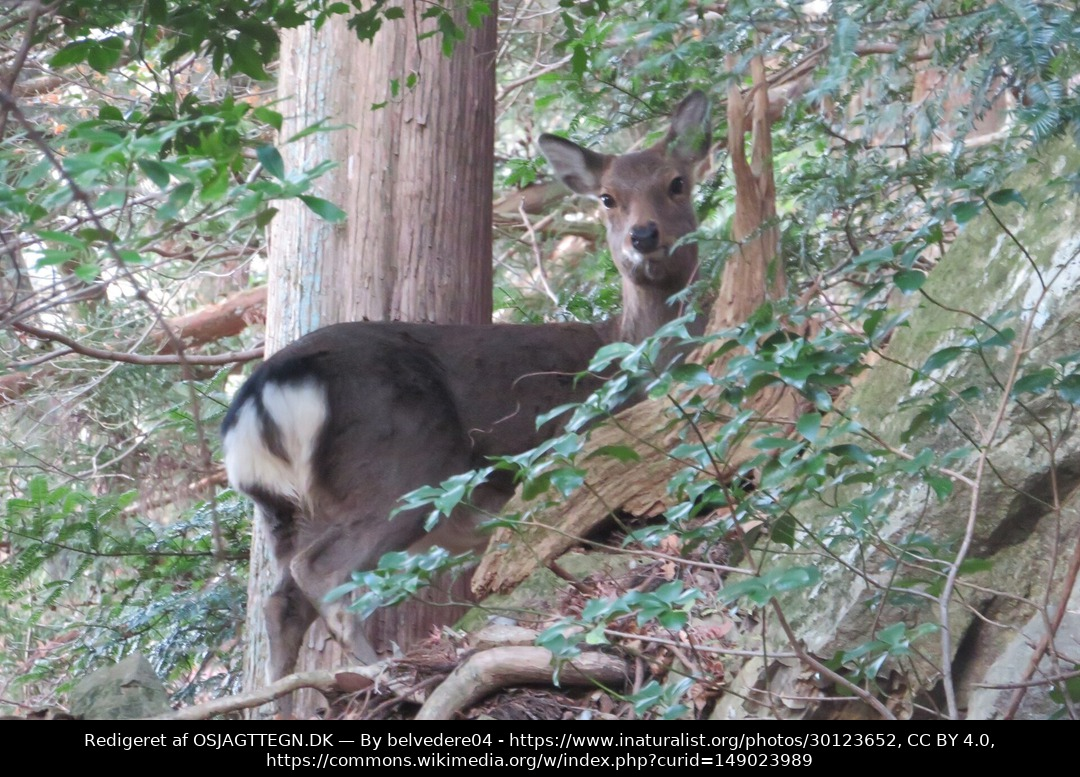
\includegraphics[width=\linewidth, height=7.2cm, keepaspectratio]{Billeder/Dyr/Pattedyr/hovdyr/sikavildt/sikavildt-female-01.jpg}
  \end{columns}
\end{frame}



\begin{frame}{Hjortevildtets spejl (rumpe)}
  \vspace{-0.3em}
  \centering
  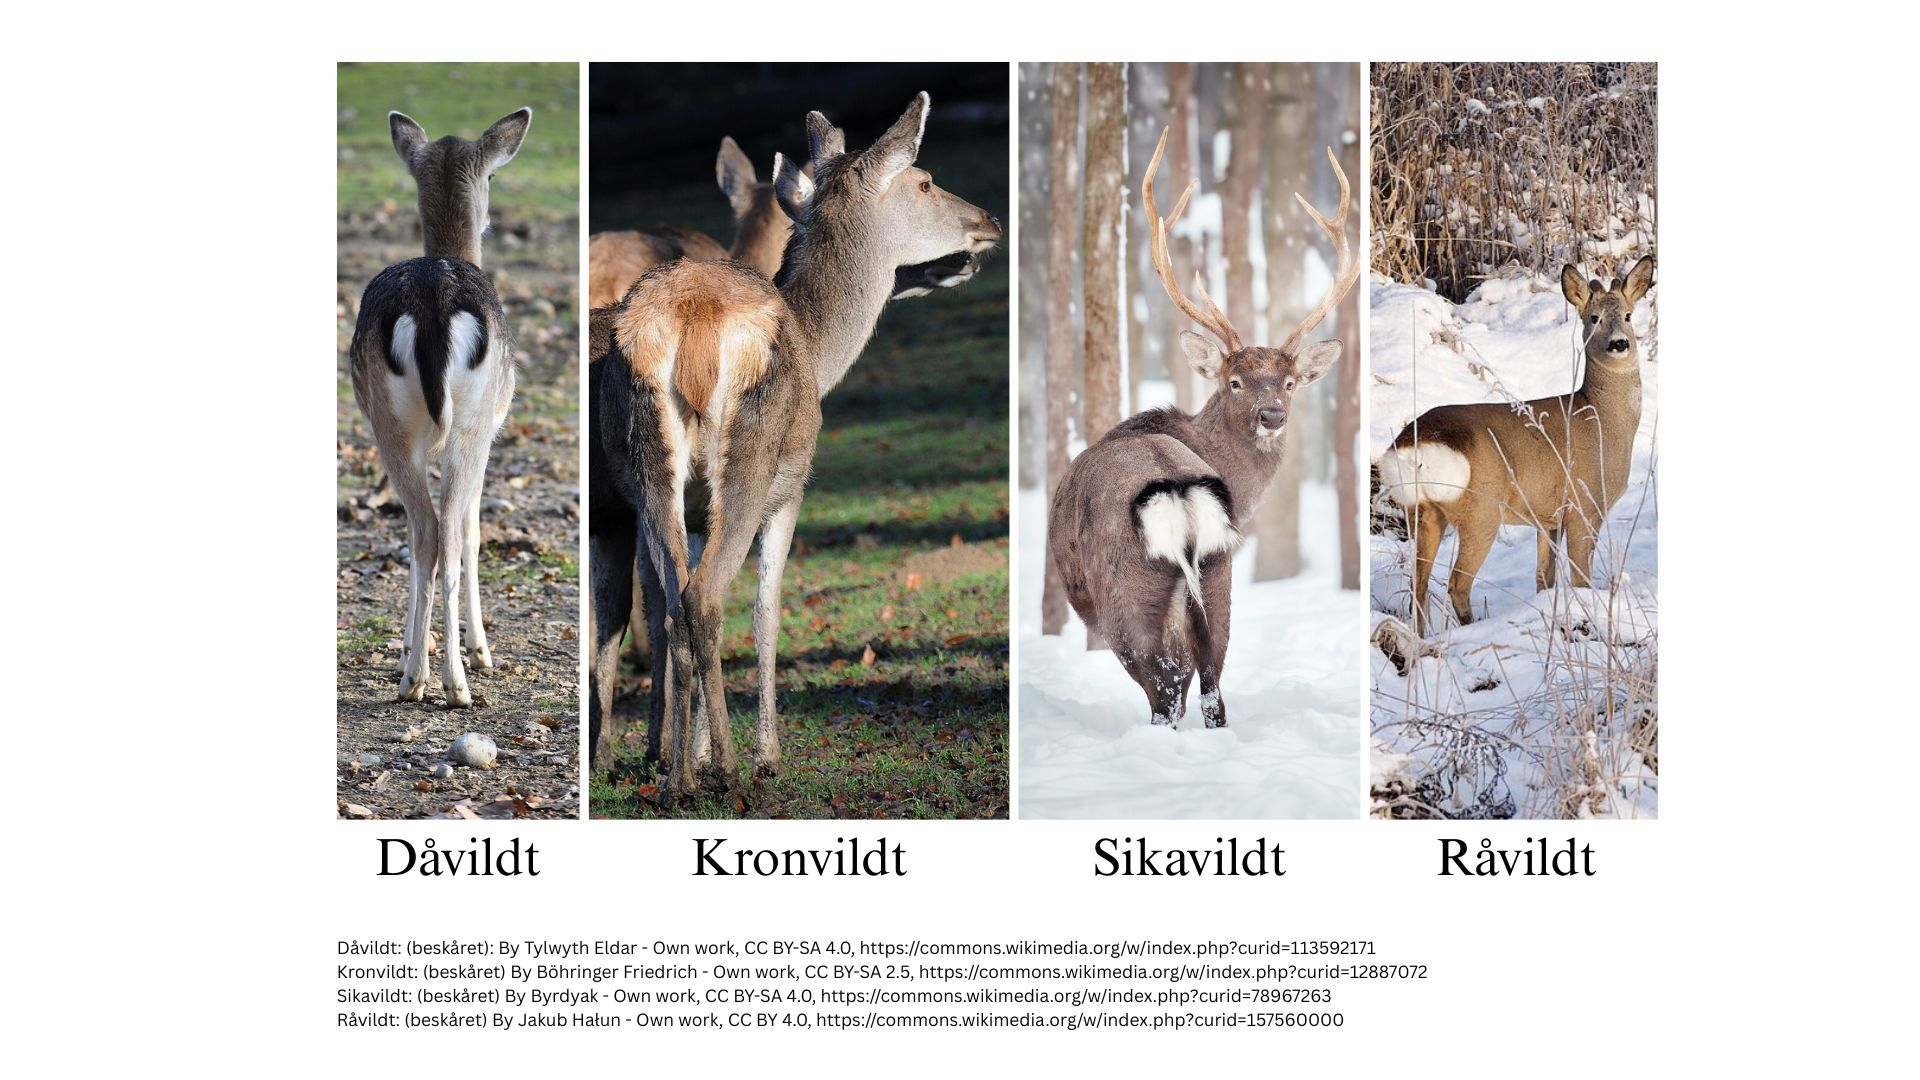
\includegraphics[width=0.95\textwidth, height=0.82\textheight, keepaspectratio]{Billeder/Dyr/Pattedyr/hovdyr/hjortevildtets_spejl.jpg}
\end{frame}

% ========== MUFLONVÆDDER ==========
\begin{frame}{%
  \begin{minipage}[c]{0.30\textwidth}
    Muflonvædder
  \end{minipage}%
  \hfill
  \begin{minipage}[c]{0.45\textwidth}
    \footnotesize
    \textbf{Jagttid:} 1.\ september -- 31.\ januar
  \end{minipage}%
  \hfill
  \begin{minipage}[c]{0.15\textwidth}
    \noindent\raggedleft
    
\includegraphics[width=0.5cm, height=0.5cm, keepaspectratio]{Billeder/Ikoner/star.png}
  \end{minipage}%
}
  \vspace{0.25em}
  \begin{columns}[T]
    \column{0.45\textwidth}
    \setlength{\parskip}{0.4em}
    \tiny
    \RaggedRight
    \textbf{\textit{Ovis musimon}} – vildt bjergfår indført til Danmark. Hannen kaldes vædder. \par
    \textbf{Udseende:}\\
    \quad – Store, bagudbøjede horn der ikke kastes, men vokser hele livet \\
    \quad – Rustrød til mørk pels med lyse saddelpletter på siden \\
    \quad – Kraftig krop og forholdsvis spinkle ben \par
    \textbf{Levesteder:} Åbne sletter, overdrev, hede og skovbryn. Trives dårligt i tæt skov. \par
    \textbf{Føde:} Græs og urter. Om vinteren også bark og stedsegrøn vegetation. \par
    \textbf{Udbredelse:} Enkelte småøer og udslip fra dyrehaver. \par
    %\textbf{Parring/brunst:} Efterår. \par
    %\textbf{Forplantning:}\\
    %\quad – \textbf{Kønsmoden:} Ca. 2--3 år \\
    %\quad – \textbf{Mono/polygam:} Polygam \\
    %\quad – \textbf{Bestandsomsætning:} Langsom \\
    %\quad – \textbf{Kuld:} 1 lam, sjældent 2
    \column{0.52\textwidth}
    \centering
    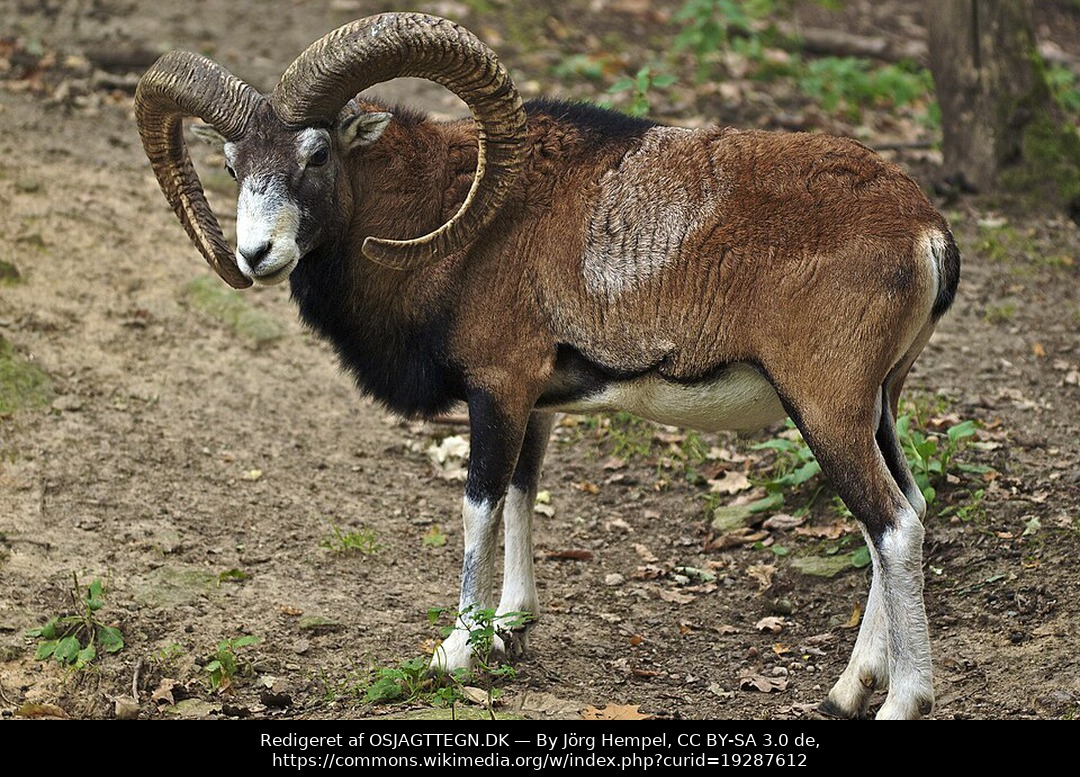
\includegraphics[width=\linewidth, height=7.2cm, keepaspectratio]{Billeder/Dyr/Pattedyr/hovdyr/muflon/muflon-male-01.jpg}
  \end{columns}
\end{frame}

% ========== MUFLONFÅR ==========
\begin{frame}{%
  \begin{minipage}[c]{0.30\textwidth}
    Muflonfår
  \end{minipage}%
  \hfill
  \begin{minipage}[c]{0.45\textwidth}
    \footnotesize
    \textbf{Jagttid:} 1.\ oktober -- 31.\ januar
  \end{minipage}%
  \hfill
  \begin{minipage}[c]{0.15\textwidth}
    \noindent\raggedleft
    
\includegraphics[width=0.5cm, height=0.5cm, keepaspectratio]{Billeder/Ikoner/star.png}
  \end{minipage}%
}
  \vspace{0.25em}
  \begin{columns}[T]
    \column{0.45\textwidth}
    \setlength{\parskip}{0.4em}
    \tiny
    \RaggedRight
    \textbf{\textit{Ovis musimon}} – hunnen hos muflon. Lever ofte i flok med lam og unge dyr. \par
    \textbf{Udseende:}\\
    \quad – Ingen eller kun korte horn \\
    \quad – Mindre end vædderen \\
    \quad – Rustrød til mørk pels, typisk uden de store lyse saddelpletter \\
    \quad – Kraftig krop og forholdsvis spinkle ben \par
    \textbf{Levesteder:} Åbne sletter, overdrev, hede og skovbryn. Trives dårligt i tæt skov. \par
    \textbf{Føde:} Græs og urter. Om vinteren også bark og stedsegrøn vegetation. \par
    \textbf{Udbredelse:} Enkelte småøer og udslip fra dyrehaver. \par
   % \textbf{Parring/brunst:} Efterår. \par
   % \textbf{Forplantning:}\\
    %\quad – \textbf{Kønsmoden:} Ca. 2 år \\
    %\quad – \textbf{Mono/polygam:} Polygam \\
    %\quad – \textbf{Bestandsomsætning:} Langsom \\
    %\quad – \textbf{Kuld:} 1 lam, sjældent 2
    \column{0.52\textwidth}
    \centering
    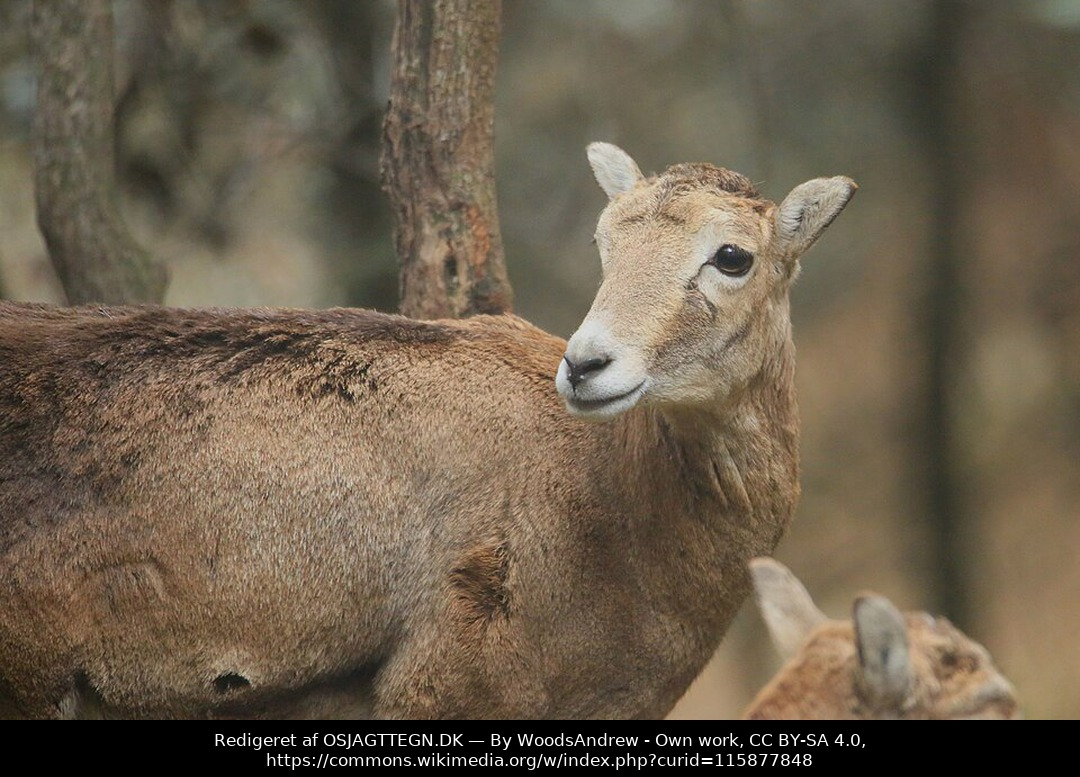
\includegraphics[width=\linewidth, height=7.2cm, keepaspectratio]{Billeder/Dyr/Pattedyr/hovdyr/muflon/muflon-female-01.jpg}
  \end{columns}
\end{frame}

% ========== VILDSVIN ==========
\begin{frame}{%
  \begin{minipage}[c]{0.30\textwidth}
    Vildsvin
  \end{minipage}%
  \hfill
  \begin{minipage}[c]{0.45\textwidth}
    \footnotesize
    \textbf{Jagttid:} Orne: 1.\ sep.--31.\ jan.\\
    So og gris: 1.\ okt.--31.\ jan.
  \end{minipage}%
  \hfill
  \begin{minipage}[c]{0.15\textwidth}
    \noindent\raggedleft
    
\includegraphics[width=0.5cm, height=0.5cm, keepaspectratio]{Billeder/Ikoner/star.png}%
    \hspace{0.2em}%
    
\includegraphics[width=0.5cm, height=0.5cm, keepaspectratio]{Billeder/Ikoner/star.png}
  \end{minipage}%
}
  \vspace{0.25em}
  \begin{columns}[T]
    \column{0.45\textwidth}
    \setlength{\parskip}{0.4em}
    \tiny
    \RaggedRight
    \textbf{\textit{Sus scrofa}} – langt, kegleformet hoved og kompakt krop med kraftig, børstet pels. Ornen har synlige hjørnetænder. \par
    \textbf{Benævnes:}\\
    \quad – Han: Orne \\
    \quad – Hun: So \\
    \quad – Unge: Gris \par
    \textbf{Udseende:}\\
    \quad – Ligner en gris \\
    \quad – Kraftig, strid pels \\
    \quad – Kompakt krop \par
    \textbf{Levesteder:} Findes i alle landskabstyper. Meget sky og nataktiv. \par
    \textbf{Føde:} Altædende, bl.a. planter, rødder, orme og ådsler. \par
    \textbf{Udbredelse:} Strejfende individer i Sydjylland. \par
    %\textbf{Forplantning:}\\
    %\quad – \textbf{Kønsmoden:} Ca. 1 år \\
    %\quad – \textbf{Mono/polygam:} Polygam \\
    %\quad – \textbf{Bestandsomsætning:} Hurtig \\
    %\quad – \textbf{Kuld:} 4--8 grise
    \column{0.52\textwidth}
    \centering
    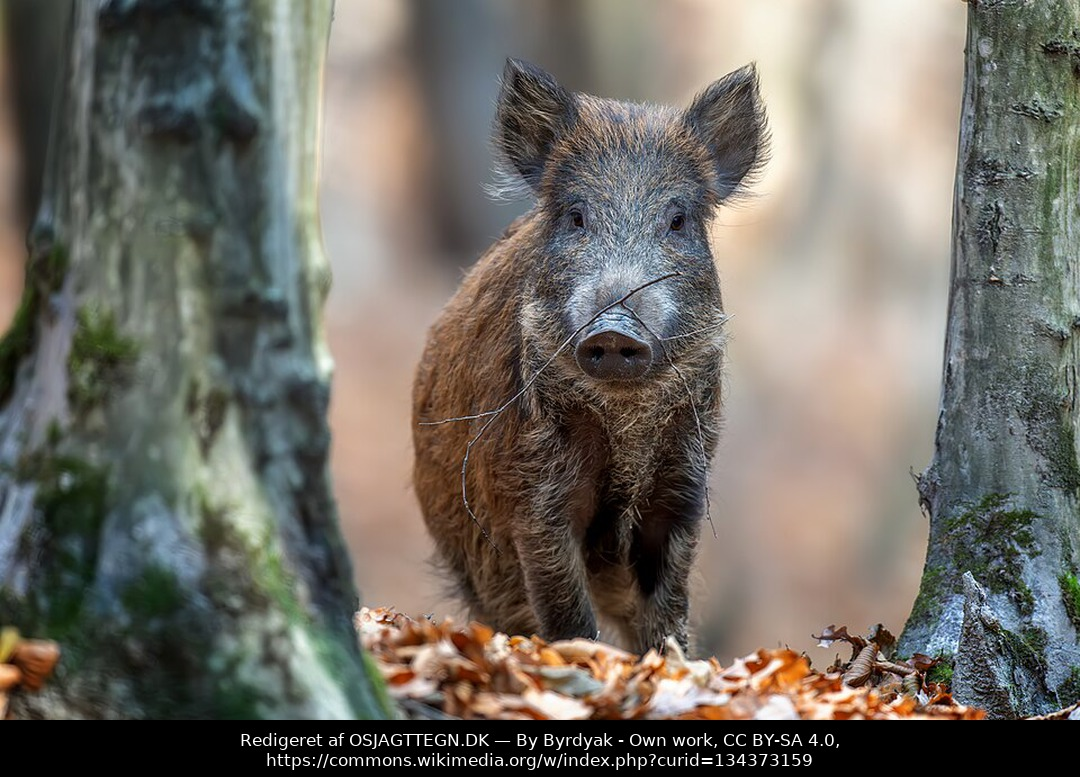
\includegraphics[width=\linewidth, height=7.2cm, keepaspectratio]{Billeder/Dyr/Pattedyr/hovdyr/vildsvin/vildsvin-01.jpg}
  \end{columns}
\end{frame}

\begin{frame}{Jagt på vildsvin}
  \vspace{-0.3em}
  \centering
  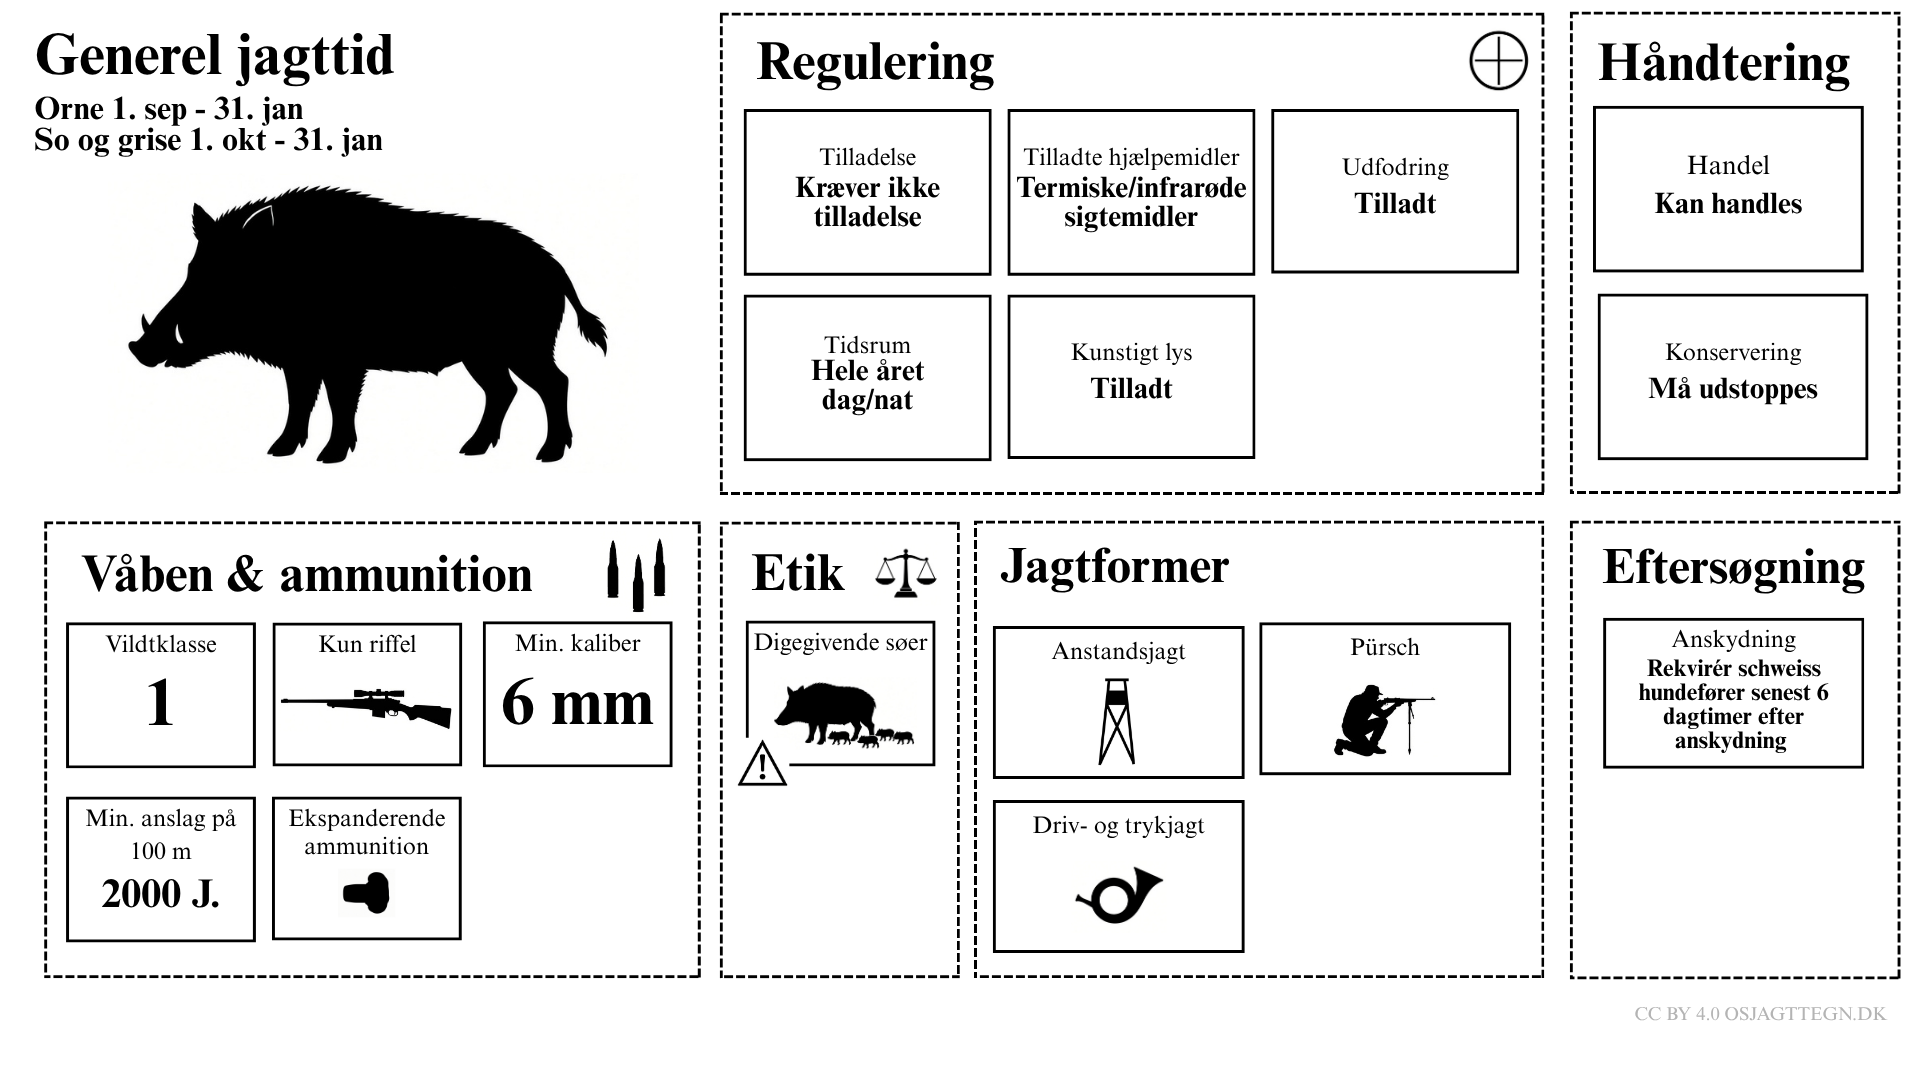
\includegraphics[width=0.95\textwidth, height=0.78\textheight, keepaspectratio]{Frames/Artsbestemmelse/Dyr/pattedyr/hovdyr/arter/vildsvin/info-vildsvin.png}
\end{frame}

%g\begin{frame}[plain]
\scriptsize
\vspace*{-1mm}

\newcommand{\ikon}[2][7mm]{%
  \IfFileExists{#2}{\includegraphics[height=#1]{#2}}{\rule{0pt}{#1}}%
}

\begin{columns}[T,onlytextwidth]
\begin{column}{0.25\textwidth}
\vspace*{4mm}
{\large\bfseries\color{myteal} Generel jagttid}\\[1mm]
{\scriptsize Orne 1.\ sep -- 31.\ jan\\
So og grise 1.\ okt -- 31.\ jan}\\[2mm]
\centering
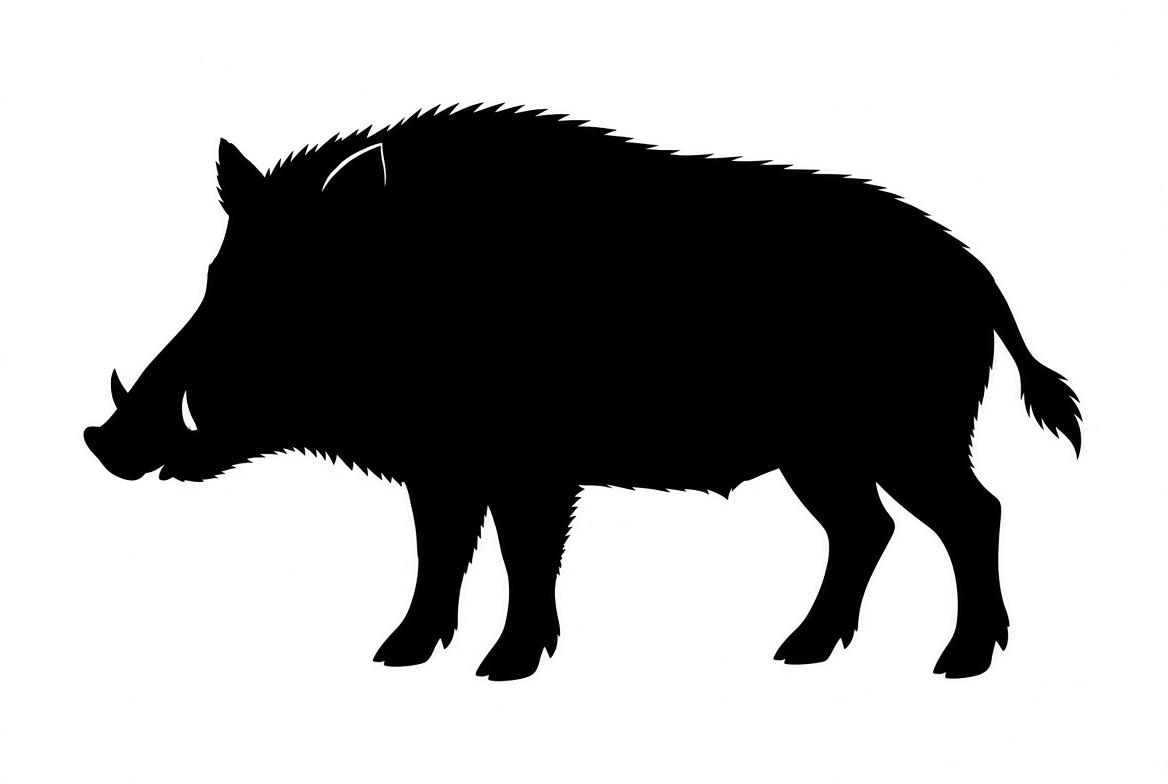
\includegraphics[width=0.95\linewidth,height=2.0cm,keepaspectratio]{Billeder/Ikoner/infografik/orne.jpg}
\end{column}

\begin{column}{0.49\textwidth}
\begin{tcolorbox}[gruppe, equal height group=toeraekke]
{\bfseries\color{myteal} Regulering}\\[0.6mm]
\begin{minipage}[t]{0.31\linewidth}
\begin{tcolorbox}[felt] Tilladelse\\ \textbf{Kræver ikke\\ tilladelse} \end{tcolorbox}
\end{minipage}\hfill
\begin{minipage}[t]{0.37\linewidth}
\begin{tcolorbox}[felt] Tilladte hjælpemidler\\ \textbf{Termiske/infr.\\ sigtemidler} \end{tcolorbox}
\end{minipage}\hfill
\begin{minipage}[t]{0.28\linewidth}
\begin{tcolorbox}[felt] Udfodring\\ \textbf{Tilladt} \end{tcolorbox}
\end{minipage}\\[0.8mm]
\begin{minipage}[t]{0.31\linewidth}
\begin{tcolorbox}[felt] Tidsrum\\ \textbf{Hele året\\ dag/nat} \end{tcolorbox}
\end{minipage}\hfill
\begin{minipage}[t]{0.37\linewidth}
\begin{tcolorbox}[felt] Kunstigt lys\\ \textbf{Tilladt} \end{tcolorbox}
\end{minipage}\hfill
\begin{minipage}[t]{0.28\linewidth}~\end{minipage}
\end{tcolorbox}
\end{column}

\begin{column}{0.24\textwidth}
\begin{tcolorbox}[gruppe, equal height group=toeraekke]
{\bfseries\color{myteal} Håndtering}\\[0.6mm]
\begin{tcolorbox}[feltfri] Handel\\ \textbf{Kan handles} \end{tcolorbox}\\[0.8mm]
\begin{tcolorbox}[feltfri] Konservering\\ \textbf{Må udstoppes} \end{tcolorbox}
\end{tcolorbox}
\end{column}
\end{columns}

\vspace{1mm}

\begin{columns}[T,onlytextwidth]
\begin{column}{0.34\textwidth}
\begin{tcolorbox}[gruppe, equal height group=bundraekke]
{\bfseries\color{myteal} Våben \& ammunition}\\[0.6mm]
\begin{minipage}[t]{0.30\linewidth}
\begin{tcolorbox}[felt] Vildtklasse\\ {\large\bfseries 1} \end{tcolorbox}
\end{minipage}\hfill
\begin{minipage}[t]{0.36\linewidth}
\begin{tcolorbox}[felt] Kun riffel\\[0.4mm]
\ikon[5mm]{Billeder/Ikoner/infografik/riffel.jpg}
\end{tcolorbox}
\end{minipage}\hfill
\begin{minipage}[t]{0.30\linewidth}
\begin{tcolorbox}[felt] Min.\ kaliber\\ \textbf{6 mm} \end{tcolorbox}
\end{minipage}\\[0.8mm]
\begin{minipage}[t]{0.48\linewidth}
\begin{tcolorbox}[felt] Min.\ anslag på 100 m\\ \textbf{2000 J.} \end{tcolorbox}
\end{minipage}\hfill
\begin{minipage}[t]{0.48\linewidth}
\begin{tcolorbox}[felt] Ekspanderende ammunition\\[0.4mm]
\ikon[5mm]{Billeder/Ikoner/infografik/ekspanderende_projektil.jpg}
\end{tcolorbox}
\end{minipage}
\end{tcolorbox}
\end{column}

\begin{column}{0.15\textwidth}
\begin{tcolorbox}[gruppe, equal height group=bundraekke]
{\bfseries\color{myteal} Etik}\\[0.6mm]
\begin{tcolorbox}[feltfri]
Digegivende søer\\[0.4mm]
\ikon[7mm]{Billeder/Ikoner/infografik/so_med_grise.jpg}\\[0.2mm]
\ikon[3mm]{Billeder/Ikoner/infografik/vær_opmærksom.jpg}
\end{tcolorbox}
\end{tcolorbox}
\end{column}

\begin{column}{0.28\textwidth}
\begin{tcolorbox}[gruppe, equal height group=bundraekke]
{\bfseries\color{myteal} Jagtformer}\\[0.6mm]
\begin{minipage}[t]{0.48\linewidth}
\begin{tcolorbox}[felt] Anstand\\[0.4mm]
\ikon[6mm]{Billeder/Ikoner/infografik/jagttårn.png}
\end{tcolorbox}
\end{minipage}\hfill
\begin{minipage}[t]{0.48\linewidth}
\begin{tcolorbox}[felt] Pürsch\\[0.4mm]
\ikon[6mm]{Billeder/Ikoner/infografik/purschjagt.jpg}
\end{tcolorbox}
\end{minipage}\\[0.8mm]
\begin{minipage}[t]{0.48\linewidth}
\begin{tcolorbox}[felt] Driv/trykjagt\\[0.4mm]
\ikon[6mm]{Billeder/Ikoner/infografik/drivjagt.jpg}
\end{tcolorbox}
\end{minipage}
\end{tcolorbox}
\end{column}

\begin{column}{0.21\textwidth}
\begin{tcolorbox}[gruppe, equal height group=bundraekke]
{\bfseries\color{myteal} Eftersøgning}\\[0.6mm]
\begin{tcolorbox}[feltfri]
Anskydning\\
\textbf{Rekvirér schweiss}\\
senest \textbf{6 dagtimer}\\
efter anskydning
\end{tcolorbox}
\end{tcolorbox}
\end{column}
\end{columns}

\vspace{1mm}
\hfill{\tiny\color{gray} CC BY 4.0 \href{https://osjagttegn.dk}{OSJAGTTEGN.DK}}
\end{frame}

\begin{frame}{Benævnelser for hovdyr}

    \small

    \begin{table}
    \centering
    \resizebox{\textwidth}{!}{
        \begin{tabular}{|l|c|c|c|c|c|c|c|}
        \hline
        \textbf{Benævnelser} & \textbf{Han} & \textbf{Hun} & \textbf{2. års han} & \textbf{2. års hun} & \textbf{Unge han} & \textbf{Unge hun} & \textbf{Flok} \\
        \hline
        \textbf{Kronvildt} & \underline{Kronhjort} & \underline{Kronhind} & \underline{Spidskronhjort} & \underline{Smalkronhind} & \multicolumn{2}{c|}{\underline{Kronkalv}} & \underline{Rudel} \\ \hline
        \textbf{Dåvildt} & \underline{Dåhjort} & \underline{Då} & \underline{Spidsdåhjort} & \underline{Smaldå} & \multicolumn{2}{c|}{\underline{Dåkalv}} & \underline{Rudel} \\ \hline
        \textbf{Sikavildt} & \underline{Sikahjort} & \underline{Sikahind} & \underline{Spidssikahjort} & \underline{Smalsikahind} & \multicolumn{2}{c|}{\underline{Sikakalv}} & \underline{Rudel} \\ \hline
        \textbf{Råvildt} & \underline{Råbuk} & \underline{Rå} & \underline{Spidsbuk} & \underline{Smalrå} & \underline{Bukkelam} & \underline{Rålam} & \underline{Spring} \\ \hline
        \textbf{Vildsvin} & \underline{Orne} \textit{(Korrekt: Keiler)} & \underline{So} & \multicolumn{2}{c|}{\textit{Overløber}} & \multicolumn{2}{c|}{\underline{Gris} \textit{(Korrekt: Grisling)}} & \textit{Rotte} \\ \hline
        \textbf{Muflon} & \underline{Vædder} & \underline{Får} & \textit{Årling} & \textit{Gimmer} & \multicolumn{2}{c|}{\underline{Lam}} & \textit{Hjord} \\ \hline
        \textit{\textbf{Elg}} & \textit{Tyr} & \textit{Ko} & \textit{Ungtyr} & \textit{Kvie} & \textit{Tyrekalv} & \textit{Kalv} & --- \\
        \hline
        \end{tabular}
    }
    \end{table}

    \vspace{0.4em}
    \tiny
    \textit{Note: Arter og benævnelser i \textit{kursiv} er ikke pensum}

\end{frame}

\begin{frame}
  \vspace{1.8em}
  \begin{center}
    \begin{minipage}{0.22\textwidth}
      \centering
      
\includegraphics[width=\linewidth]{Billeder/Dyr/Pattedyr/hovdyr/hovdyr_qr.png}
    \end{minipage}%
    \hspace{0.8em}%
    \begin{minipage}{0.62\textwidth}
      \raggedright
      \Large
      \textbf{Træning i artsbestemmelse af hovdyr}\\[0.35em]
      {\large https://osjagttegn.dk/hovdyr}
    \end{minipage}
  \end{center}
\end{frame}


\section{Jagtetiske regler}

\begin{frame}
  \vspace{3em}
  \begin{center}
    {\LARGE \textbf{Jagtetiske regler}}
    \\
    \vspace{1em}
    Danmarks Jægerforbund, Naturstyrelsen, Vildtforvaltningsrådet
  \end{center}
\end{frame}

\begin{frame}{Generelle hensyn – Jagtens omdømme \& etik}
\begin{itemize}
\item Alt jagt skal følge lovgivning samt jagtetiske regler
\item Jagt er mere end skydning – anvend nedlagt vildt mest muligt (føde, pels, trofæ)
\item Vildt behandles med respekt – også uanvendeligt vildt (nedgravning/destruktion)
\item Efterlad naturen uden spor – tag alt affald med
\item Undgå jagt på udsat vildt med unaturlig adfærd
\item Kun nødvendig fodring – ænder primært korn/frø på land
\item Forsøg at være et forbillede – lær af erfarne jægere
\end{itemize}
\end{frame}

\begin{frame}{Hensyn til vildtbestandene}
\begin{itemize}
\item Jag kun en del af det naturlige overskud – brug forsigtighedsprincippet
\item Kend dit vildt – skyd kun når du er sikker på arten
\item Tilpas jagttryk til terrænets bæreevne – ikke til leje eller antal jægere
\item Trækkende vildt = fælles ansvar – skån hvileområder og fouragering
\item Begræns forstyrrelser: max 3–4 klap-/drivjagt pr. sæson pr. areal
\item Minimum 2–3 ugers interval mellem jagter på samme lokalitet
\item Afbalanceret afskydning (køn, alder) – forvalt som du ønsker naboen gør det
\end{itemize}
\end{frame}

\begin{frame}{Hensyn til individet – Effektiv aflivning}
\begin{itemize}
\item Brug korrekt våben/ammunition – indskyd og træn regelmæssigt
\item Respektér dine skydebegrænsninger – træn på banen, ikke på jagt!
\item Maks. afstande hagljagt (forsigtige anbefalinger):
  \begin{itemize}
  \item Råvildt 20 m \quad Gæs/ræv 25 m \quad Øvrigt 30 m
  \end{itemize}
\item Riffel: Fast anlæg – max 100 m – frit skudfelt – ingen hals/hovedskud
\item Kun ét mål ad gangen – ingen skift af dyr ved anskydning
\item Saml alt op – eftersøg ihærdigt – hjælp hinanden
\end{itemize}
\end{frame}

\begin{frame}{Praktiske skudregler \& eftersøgning}
\begin{itemize}
\item Hagl: max $\sim$3 patroner pr. flyvende fugl, $\sim$2 pr. løbende vildt
\item Riffel: skudantal $\approx$ antal nedlagt vildt
\item Hold øje med anskudt vildt – marker præcist – instruer hundefører
\item Havjagt: forfølg dykkende anskudte vedholdende – stop jagt ved vanskelige forhold
\item Affang anskudt vildt hurtigt og dyreværnsmæssigt korrekt
\item Aldrig dublé råvildt med hagl – begræns dublé i øvrigt
\end{itemize}
\end{frame}

\begin{frame}{Hensyn til andre naturbrugere}
\begin{itemize}
\item Vær venlig og vejled ift. jagtaktivitet – irettesæt kun når nødvendigt
\item Undgå unødvendig lukning af skov – brug vejledende skilte
\item Stor forsigtighed med haglnedfald nær andre mennesker
\item Jag ikke hvor det er til klar ulempe for andre
\item Strand-/havjagt: hold god afstand til alle andre brugere
\end{itemize}
\end{frame}

\begin{frame}{Hensyn til medjægere \& nabosamarbejde}
\begin{itemize}
\item Respektér andres jagtret – samarbejd med nabojægere
\item Aftal jagthyppighed, afskydning og eftersøgning
\item Skyd aldrig vildt der drives fra naboterræn
\item Påtal ulovlig eller uetisk jagt – altid
\item Vis storsind ved tvivl om vildtets tilhørsforhold
\item Sikker våbenhåndtering – altid
\end{itemize}
\end{frame}

\begin{frame}{Sikkerhed}
\begin{itemize}
\item Røde hattebånd / høj synlighed – sikkerhedsbriller ved hagl
\item Våben uladt, knækket/åben, lodret mellem poster
\item Minimum 40$^{\circ}$ sikkerhedsvinkel – ekstra forsigtighed ved rikochet
\item Ingen lav skydning mod uoverskuelig baggrund
\item Riffel: altid sikkert kuglefang
\item Strand-/havjagt: moderne sikkerhedsudstyr – ingen unødige chancer
\item Følg Søsportens Sikkerhedsråds anbefalinger
\end{itemize}
\end{frame}
\section{Rovdyr (Artsbestemmelse \& biologi)}

% ========== TITEL: ROVDYR ==========
\begin{frame}
  \vspace{1.5em}
  \begin{center}
    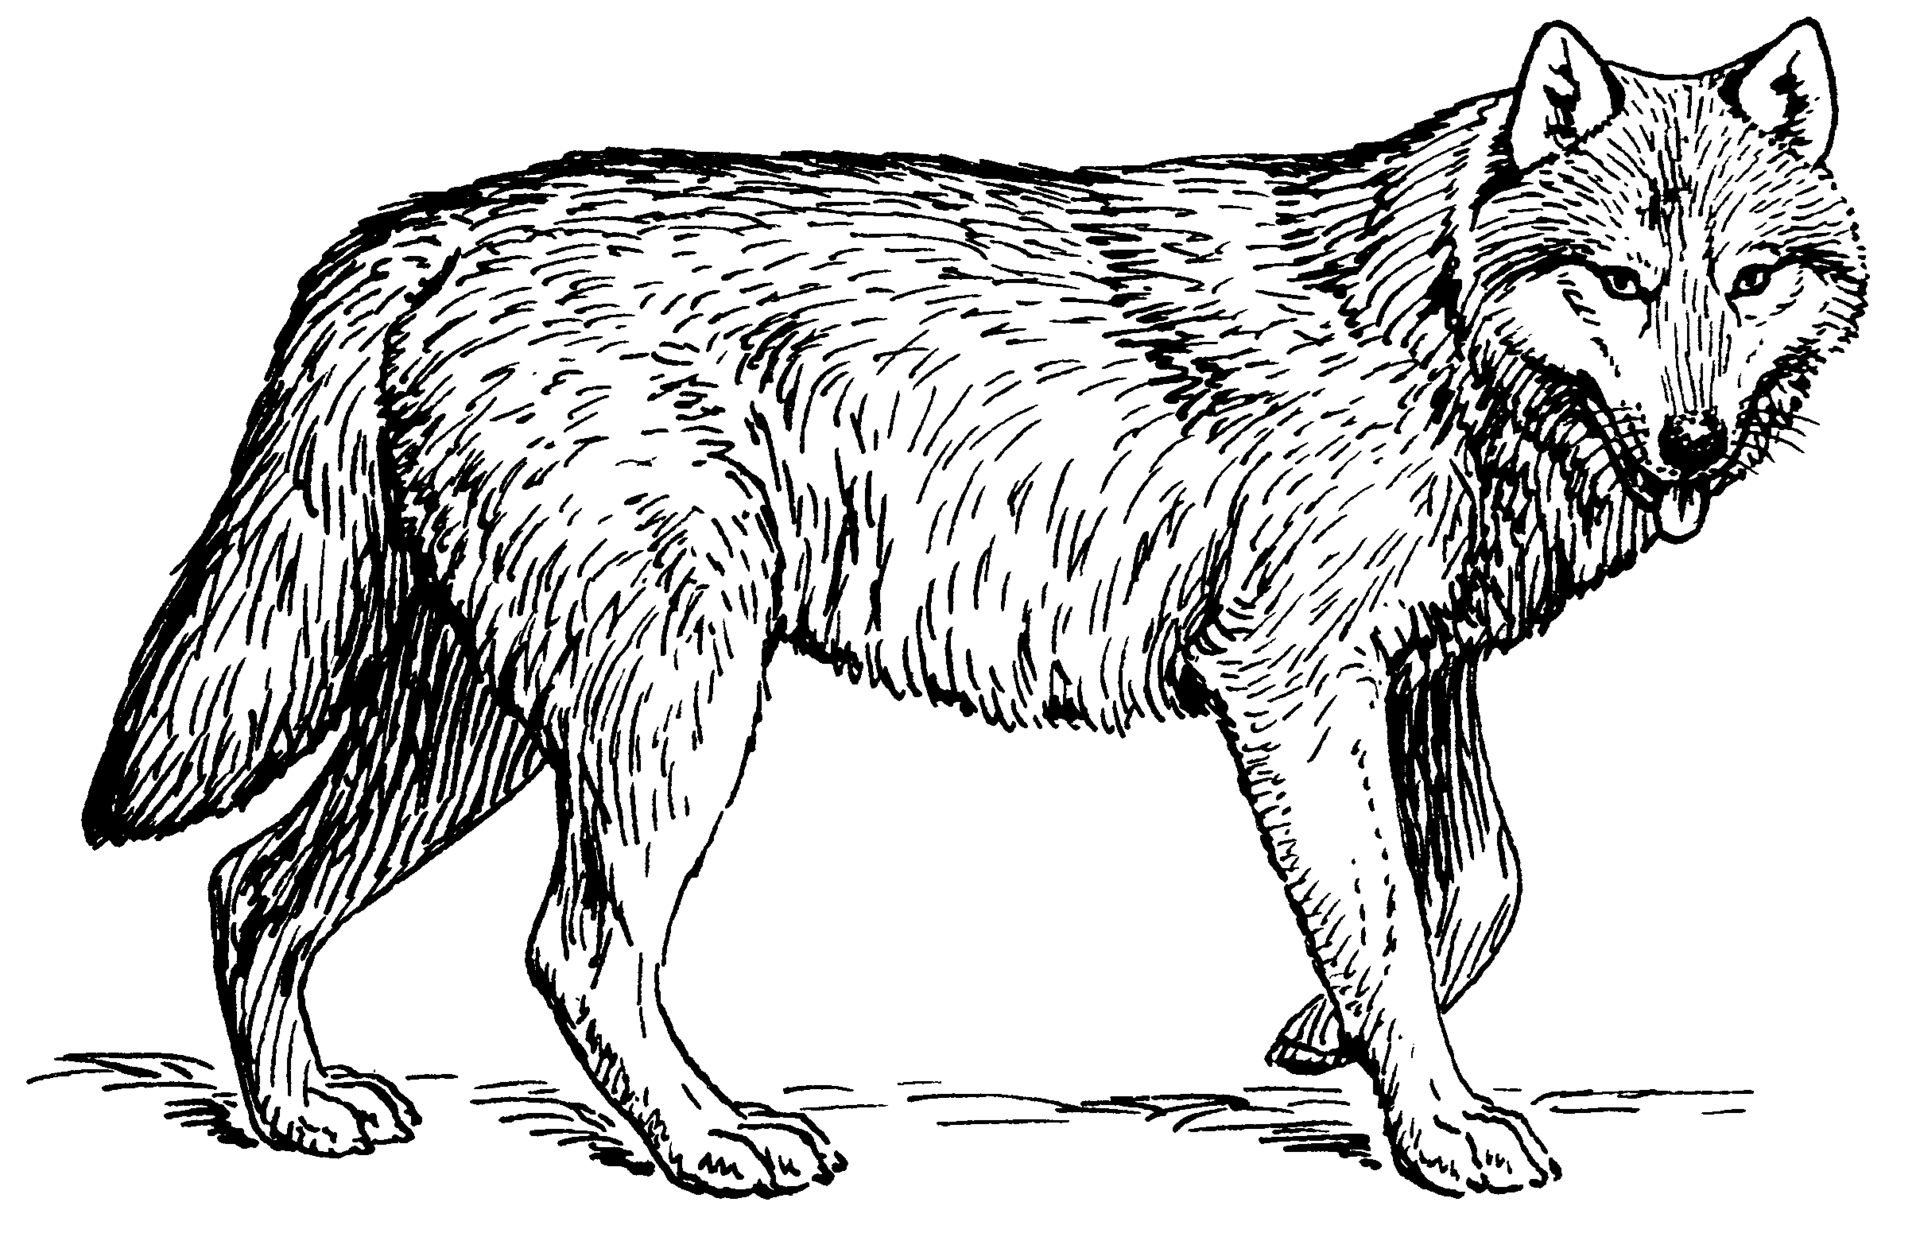
\includegraphics[width=12cm, height=4cm, keepaspectratio]{Billeder/Dyr/Pattedyr/rovdyr/rovdyr.png}\\[1.2em]
    {\LARGE \textbf{Rovdyr}}\\[0.6em]
    
    Artsbestemmelse \& vildtbiologi  \\[0.9em]
    {\tiny\color{gray}
    CC BY 4.0 – kan frit anvendes, også kommercielt. Rettighederne må ikke skærpes.\\[0.05em]
    Udviklet af Aleksander Sønder, OSJAGTTEGN.DK}
  \end{center}
\end{frame}

% ========== RÆV ==========
\begin{frame}{%
  \begin{minipage}[c]{0.30\textwidth}
    Ræv
  \end{minipage}%
  \hfill
  \begin{minipage}[c]{0.45\textwidth}
    \footnotesize
    \textbf{Jagttid:} 1.\ september -- 31.\ januar
  \end{minipage}%
  \hfill
  \begin{minipage}[c]{0.15\textwidth}
    \noindent\raggedleft
    
\includegraphics[width=0.5cm, height=0.5cm, keepaspectratio]{Billeder/Ikoner/star.png}%
    \hspace{0.2em}%
    
\includegraphics[width=0.5cm, height=0.5cm, keepaspectratio]{Billeder/Ikoner/star.png}%
    \hspace{0.2em}%
    
\includegraphics[width=0.5cm, height=0.5cm, keepaspectratio]{Billeder/Ikoner/star.png}
  \end{minipage}%
}
  \vspace{0.25em}
  \begin{columns}[T]
    % --- Venstre kolonne: Tekst ---
    \column{0.45\textwidth}
    \setlength{\parskip}{0.4em}
    \tiny
    \RaggedRight
    \textbf{\textit{Vulpes vulpes}} – udbredt hundedyr, der er ekstremt tilpasningsdygtigt og ses overalt i Danmark. \par
    \textbf{Udseende:}\\
    \quad – Overvejende rød \\
    \quad – Hvid bug \\
    \quad – Markant rød hale \\
    \quad – Sorte aftegninger \par
    \textbf{Levesteder:} Alle landskabstyper. \par
    \textbf{Føde:} Smågnavere, fugle, bær, biller, ådsler, harekillinger og rålam. \par
    \textbf{Sygdomme:} Ræveskab, rævens dværgbændelorm, hvalpesyge. \par
    \textbf{Parring:} Sidst i januar / start februar (rolletiden). \par
    \textbf{Forplantning:}\\
    \quad – \textbf{Kønsmoden:} 1 år \\
    \quad – \textbf{Mono/polygam:} Monogam \\
    \quad – \textbf{Bestandsomsætning:} Middel \\
    \quad – \textbf{Kuld:} 4--7 hvalpe
    % --- Højre kolonne: Større billede ---
    \column{0.52\textwidth}
    \centering
    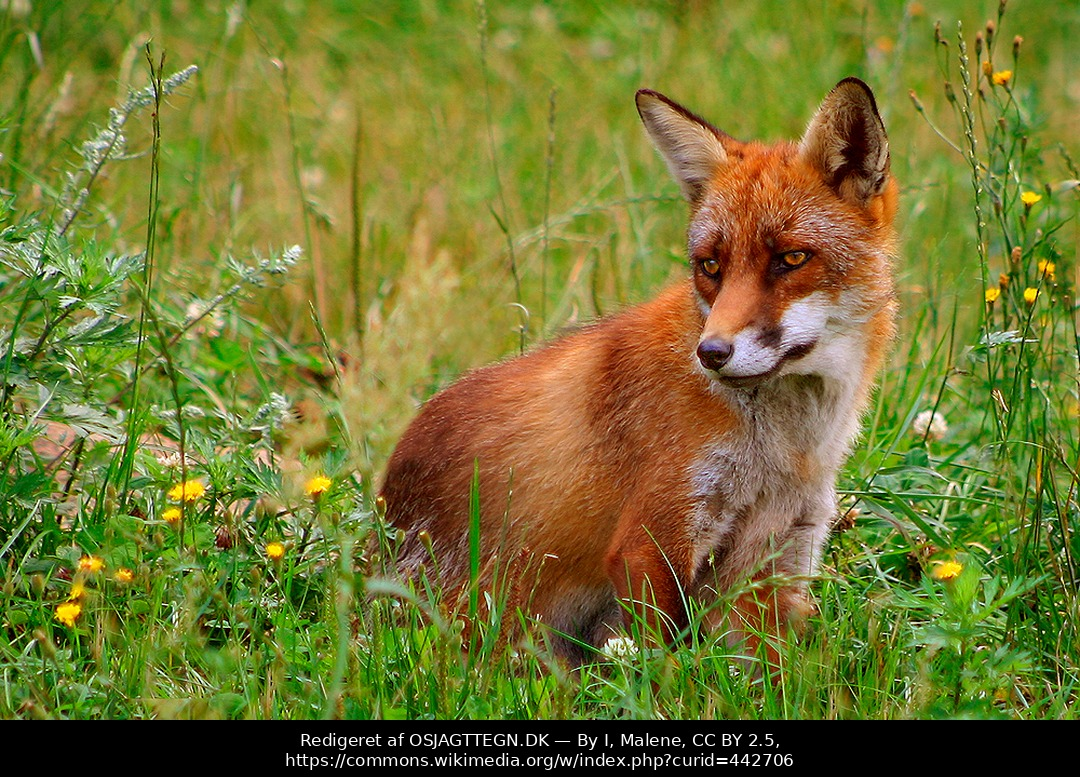
\includegraphics[width=\linewidth, height=7.2cm, keepaspectratio]{Billeder/Dyr/Pattedyr/rovdyr/ræv/raev-10.jpg}
  \end{columns}
\end{frame}

% ========== MÅRHUND ==========
\begin{frame}{%
  \begin{minipage}[c]{0.30\textwidth}
    Mårhund
  \end{minipage}%
  \hfill
  \begin{minipage}[c]{0.45\textwidth}
    \footnotesize
    \textbf{Jagttid:} 1. sep -- 31. jan\\
    \textbf{Regulering:} Uden aftale (invasiv)
  \end{minipage}%
  \hfill
  \begin{minipage}[c]{0.15\textwidth}
    \noindent\raggedleft
    
\includegraphics[width=0.5cm, height=0.5cm, keepaspectratio]{Billeder/Ikoner/star.png}%
    \hspace{0.2em}%
    
\includegraphics[width=0.5cm, height=0.5cm, keepaspectratio]{Billeder/Ikoner/star.png}
  \end{minipage}%
}
  \vspace{0.25em}
  \begin{columns}[T]
    % --- Venstre kolonne: Tekst ---
    \column{0.45\textwidth}
    \setlength{\parskip}{0.4em}
    \tiny
    \RaggedRight
    \textbf{\textit{Nyctereutes procyonoides}} – invasivt hundedyr, der er ekstremt tilpasningsdygtigt. \par
    \textbf{Udseende:}\\
    \quad – Mørk med lange dækhår \\
    \quad – Bryst, ben og underside er sort \\
    \quad – Ansigtsmaske med brede sorte striber over øjnene \par
    \textbf{Levesteder:} Alle landskabstyper. \par
    \textbf{Føde:} Små pattedyr, fugle, fisk, bær, biller, ådsler, affald. \par
    \textbf{Udbredelse:} Primært Jylland.
    % --- Højre kolonne: Større billede ---
    \column{0.52\textwidth}
    \centering
    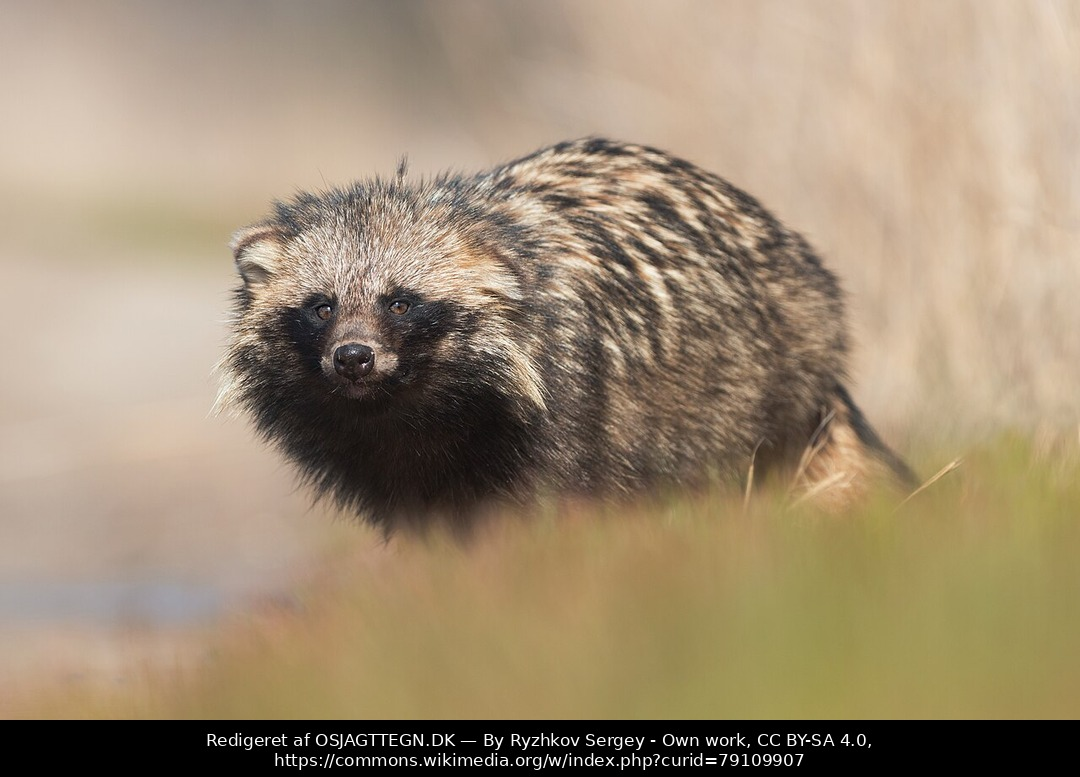
\includegraphics[width=\linewidth, height=7.2cm, keepaspectratio]{Billeder/Dyr/Pattedyr/rovdyr/mårhund/maarhund-01.jpg}
  \end{columns}
\end{frame}

% ========== MINK ==========
\begin{frame}{%
  \begin{minipage}[c]{0.30\textwidth}
    Mink
  \end{minipage}%
  \hfill
  \begin{minipage}[c]{0.45\textwidth}
    \footnotesize
    \textbf{Jagttid:} 1. sep -- 31. jan\\
    \textbf{Regulering:} Uden aftale (invasiv)
  \end{minipage}%
  \hfill
  \begin{minipage}[c]{0.15\textwidth}
    \noindent\raggedleft
    
\includegraphics[width=0.5cm, height=0.5cm, keepaspectratio]{Billeder/Ikoner/star.png}%
    \hspace{0.2em}%
    
\includegraphics[width=0.5cm, height=0.5cm, keepaspectratio]{Billeder/Ikoner/star.png}
  \end{minipage}%
}
  \vspace{0.25em}
  \begin{columns}[T]
    % --- Venstre kolonne: Tekst ---
    \column{0.45\textwidth}
    \setlength{\parskip}{0.4em}
    \tiny
    \RaggedRight
    \textbf{\textit{Neogale vison}} – undslupne dyr fra pelsavl har etableret sig langs kysterne mange steder i Danmark. \par
    \textbf{Udseende:}\\
    \quad – Mørk, ensfarvet pels \\
    \quad – Vilde mink kan være lysere ved hovedet \\
    \quad – Ingen maske som ilderen \par
    \textbf{Levesteder:} I nærheden af vand. \par
    \textbf{Føde:} Fisk, smågnavere, fugle, krabber, padder og insekter. \par
    \textbf{Udbredelse:} Hele landet undtagen småøer.
    % --- Højre kolonne: Større billede ---
    \column{0.52\textwidth}
    \centering
    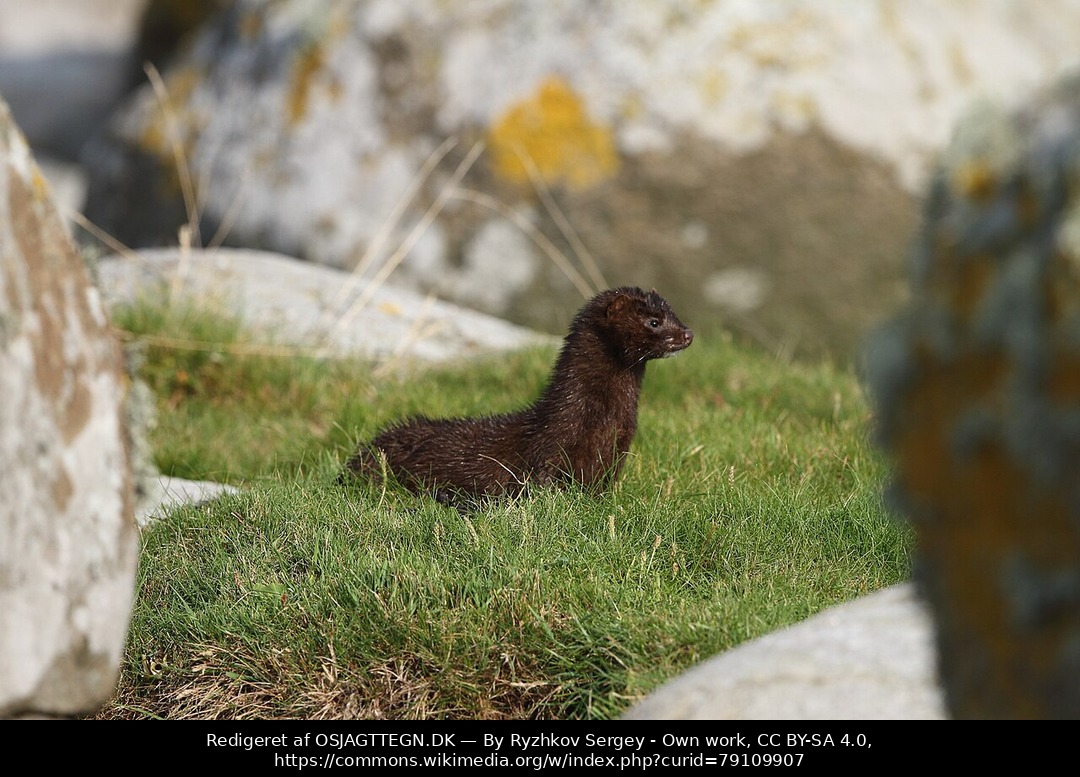
\includegraphics[width=\linewidth, height=7.2cm, keepaspectratio]{Billeder/Dyr/Pattedyr/rovdyr/mink/mink-01.jpg}
  \end{columns}
\end{frame}

% ========== HUSMÅR ==========
\begin{frame}{%
  \begin{minipage}[c]{0.30\textwidth}
    Husmår
  \end{minipage}%
  \hfill
  \begin{minipage}[c]{0.45\textwidth}
    \footnotesize
    \textbf{Jagttid:} 1.\ september -- 31.\ januar
  \end{minipage}%
  \hfill
  \begin{minipage}[c]{0.15\textwidth}
    \noindent\raggedleft
    
\includegraphics[width=0.5cm, height=0.5cm, keepaspectratio]{Billeder/Ikoner/star.png}%
    \hspace{0.2em}%
    
\includegraphics[width=0.5cm, height=0.5cm, keepaspectratio]{Billeder/Ikoner/star.png}
  \end{minipage}%
}
  \vspace{0.25em}
  \begin{columns}[T]
    % --- Venstre kolonne: Tekst ---
    \column{0.45\textwidth}
    \setlength{\parskip}{0.4em}
    \tiny
    \RaggedRight
    \textbf{\textit{Martes foina}} – har sit navn, da den ofte tager ophold ved menneskelig bebyggelse. \par
    \textbf{Udseende:}\\
    \quad – Rødbrun pels \\
    \quad – Hvid halsplet som deler sig ned over forbenene \par
    \textbf{Levesteder:} Ved menneskelig bebyggelse, sommerhuskvarterer og villaområder. \par
    \textbf{Føde:} Smågnavere, spurvefugle, hare, muldvarp, pindsvin. \par
    \textbf{Udbredelse:} Hele landet undtagen Bornholm og småøer.
    % --- Højre kolonne: Større billede ---
    \column{0.52\textwidth}
    \centering
    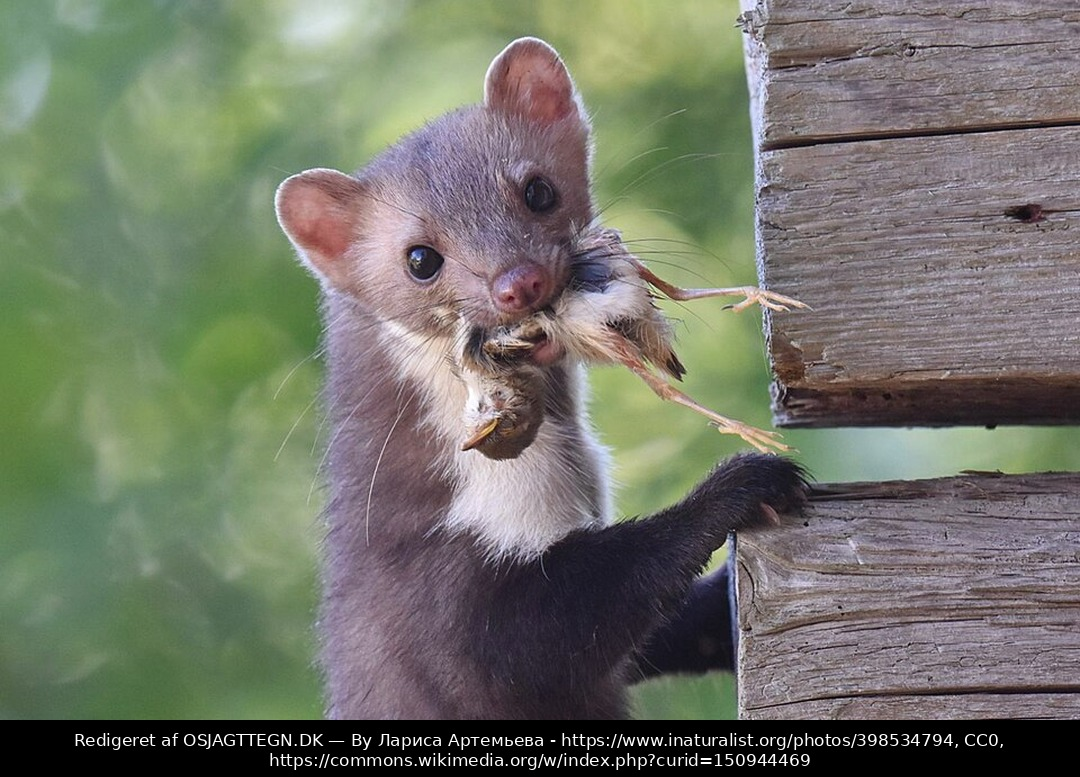
\includegraphics[width=\linewidth, height=7.2cm, keepaspectratio]{Billeder/Dyr/Pattedyr/rovdyr/husmår/husmaar-03.jpg}
  \end{columns}
\end{frame}

% ========== GRÆVLING ==========
\begin{frame}{%
  \begin{minipage}[c]{0.30\textwidth}
    Grævling
  \end{minipage}%
  \hfill
  \begin{minipage}[c]{0.45\textwidth}
    \footnotesize
    \textbf{Jagttid:} Ingen jagttid
  \end{minipage}%
  \hfill
  \begin{minipage}[c]{0.15\textwidth}
    \noindent\raggedleft
    
\includegraphics[width=0.5cm, height=0.5cm, keepaspectratio]{Billeder/Ikoner/star.png}
  \end{minipage}%
}
  \vspace{0.25em}
  \begin{columns}[T]
    % --- Venstre kolonne: Tekst ---
    \column{0.45\textwidth}
    \setlength{\parskip}{0.4em}
    \tiny
    \RaggedRight
    \textbf{\textit{Meles meles}} – pæreformet krop med sort-hvide striber på langs af hoved og hals. \par
    \textbf{Udseende:}\\
    \quad – Pæreformet krop \\
    \quad – Sort-hvide længdestriber i ansigtet
    % --- Højre kolonne: Større billede ---
    \column{0.52\textwidth}
    \centering
    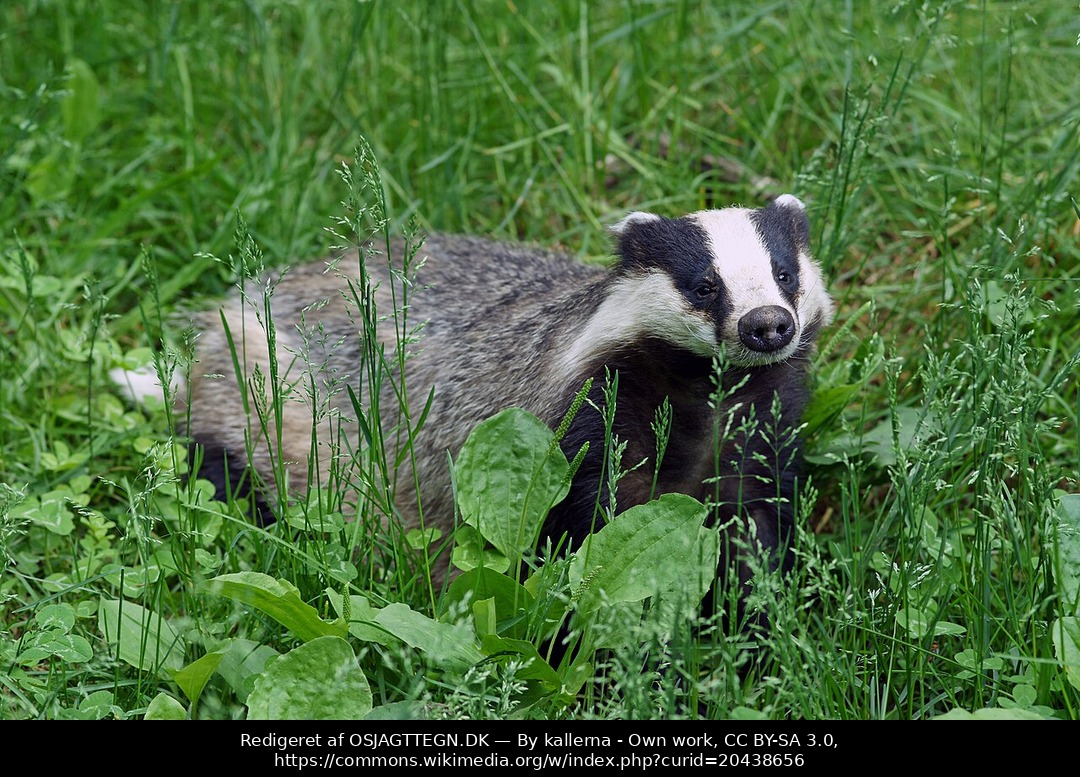
\includegraphics[width=\linewidth, height=7.2cm, keepaspectratio]{Billeder/Dyr/Pattedyr/rovdyr/grævling/graevling-01.jpg}
  \end{columns}
\end{frame}

% ========== ILDER ==========
\begin{frame}{%
  \begin{minipage}[c]{0.30\textwidth}
    Ilder
  \end{minipage}%
  \hfill
  \begin{minipage}[c]{0.45\textwidth}
    \footnotesize
    \textbf{Jagttid:} Ingen jagttid
  \end{minipage}%
  \hfill
  \begin{minipage}[c]{0.15\textwidth}
    \noindent\raggedleft
    
\includegraphics[width=0.5cm, height=0.5cm, keepaspectratio]{Billeder/Ikoner/star.png}
  \end{minipage}%
}
  \vspace{0.25em}
  \begin{columns}[T]
    % --- Venstre kolonne: Tekst ---
    \column{0.45\textwidth}
    \setlength{\parskip}{0.4em}
    \tiny
    \RaggedRight
    \textbf{\textit{Mustela putorius}} – lille mårart med karakteristisk mørk røvermaske omkring øjnene. \par
    \textbf{Udseende:}\\
    \quad – Mørk røvermaske omkring øjnene \\
    \quad – Lange, mørke dækhår
    % --- Højre kolonne: Større billede ---
    \column{0.52\textwidth}
    \centering
    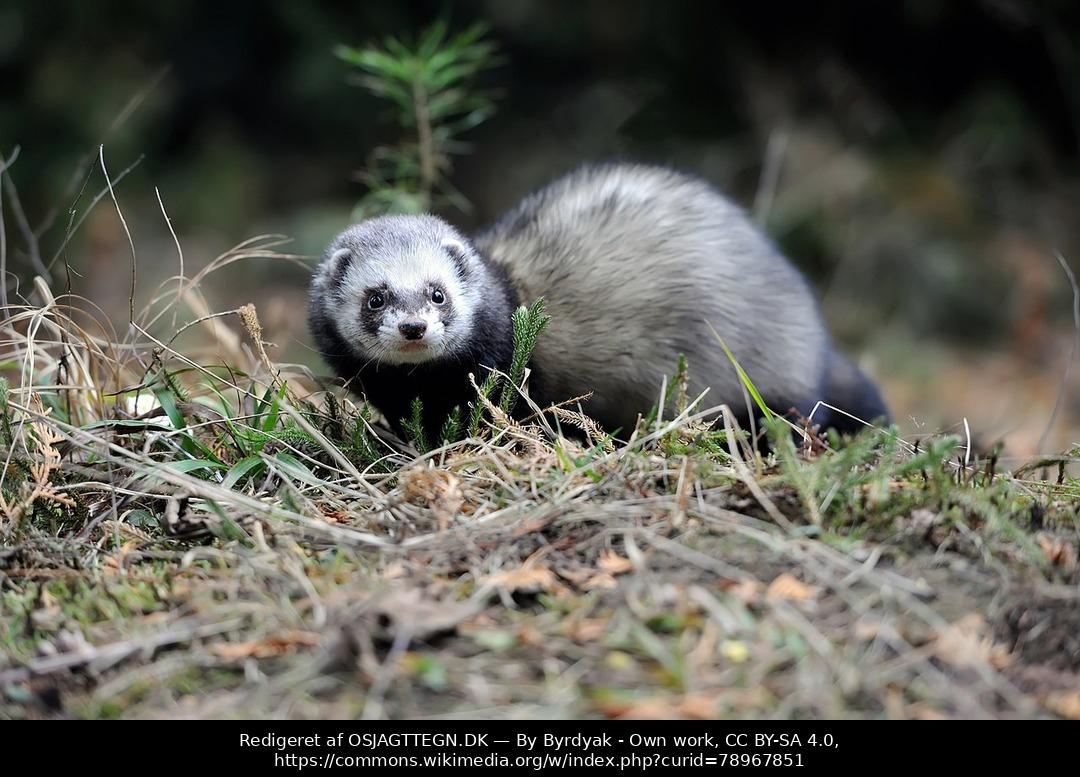
\includegraphics[width=\linewidth, height=7.2cm, keepaspectratio]{Billeder/Dyr/Pattedyr/rovdyr/ilder/ilder-01.jpg}
  \end{columns}
\end{frame}

% ========== LÆKAT ==========
\begin{frame}{%
  \begin{minipage}[c]{0.30\textwidth}
    Lækat
  \end{minipage}%
  \hfill
  \begin{minipage}[c]{0.45\textwidth}
    \footnotesize
    \textbf{Jagttid:} Ingen jagttid
  \end{minipage}%
  \hfill
  \begin{minipage}[c]{0.15\textwidth}
    \noindent\raggedleft
    
\includegraphics[width=0.5cm, height=0.5cm, keepaspectratio]{Billeder/Ikoner/star.png}
  \end{minipage}%
}
  \vspace{0.25em}
  \begin{columns}[T]
    % --- Venstre kolonne: Tekst ---
    \column{0.45\textwidth}
    \setlength{\parskip}{0.4em}
    \tiny
    \RaggedRight
    \textbf{\textit{Mustela erminea}} – lille mårart. Om vinteren er den helt hvid og kaldes hermelin. \par
    \textbf{Udseende:}\\
    \quad – Oversiden rødbrun, undersiden lys/hvid \\
    \quad – Om vinteren helt hvid (hermelin) \\
    \quad – Sort halespids hele året
    % --- Højre kolonne: Større billede ---
    \column{0.52\textwidth}
    \centering
    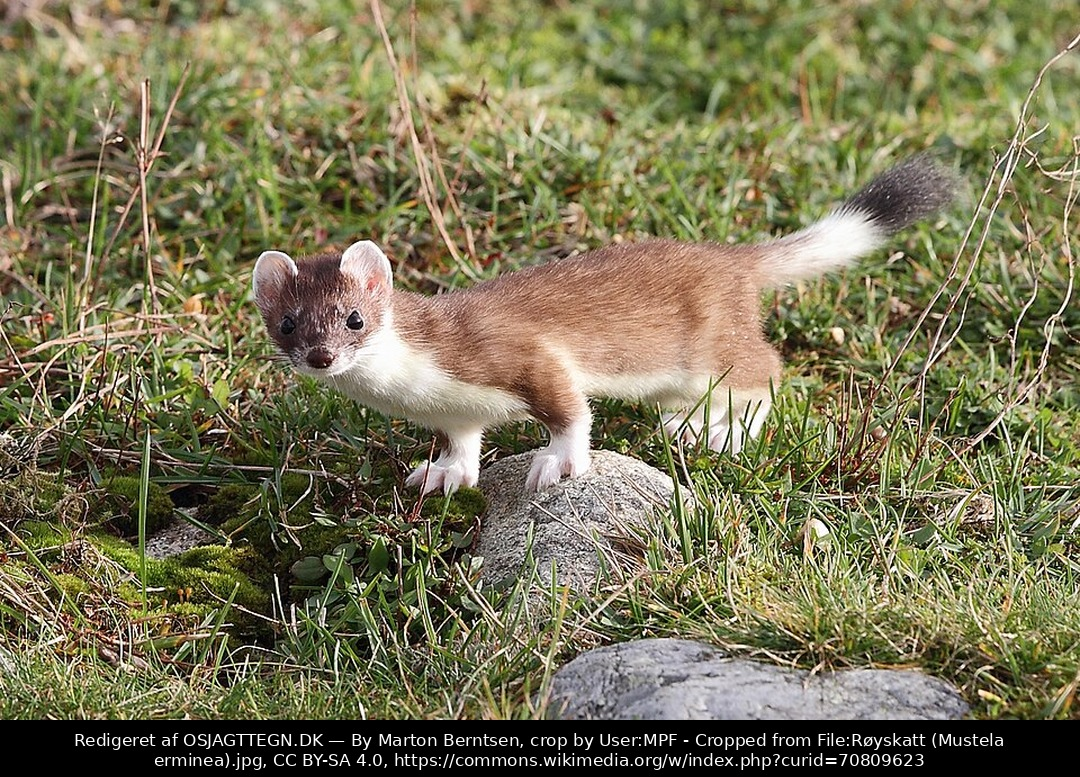
\includegraphics[width=\linewidth, height=7.2cm, keepaspectratio]{Billeder/Dyr/Pattedyr/rovdyr/lækat/laekat-02.jpg}
  \end{columns}
\end{frame}

% ========== ODDER ==========
\begin{frame}{%
  \begin{minipage}[c]{0.30\textwidth}
    Odder
  \end{minipage}%
  \hfill
  \begin{minipage}[c]{0.45\textwidth}
    \footnotesize
    \textbf{Jagttid:} Ingen jagttid
  \end{minipage}%
  \hfill
  \begin{minipage}[c]{0.15\textwidth}
    \noindent\raggedleft
    
\includegraphics[width=0.5cm, height=0.5cm, keepaspectratio]{Billeder/Ikoner/star.png}
  \end{minipage}%
}
  \vspace{0.25em}
  \begin{columns}[T]
    % --- Venstre kolonne: Tekst ---
    \column{0.45\textwidth}
    \setlength{\parskip}{0.4em}
    \tiny
    \RaggedRight
    \textbf{\textit{Lutra lutra}} – vandtilpasset mårart, der kan minde om et lille sællignende dyr. \par
    \textbf{Udseende:}\\
    \quad – Mørkebrun pels med tæt underuld \\
    \quad – Kan være hvidgrå \\
    \quad – Lang krop og hale, korte ben
    % --- Højre kolonne: Større billede ---
    \column{0.52\textwidth}
    \centering
    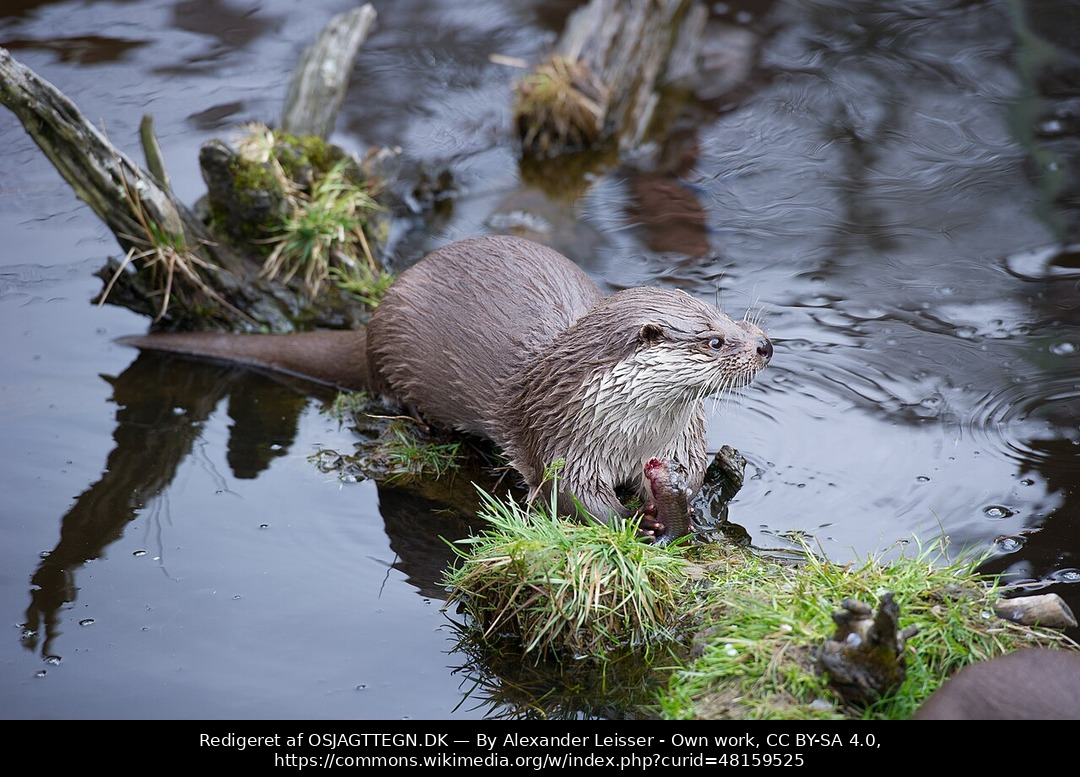
\includegraphics[width=\linewidth, height=7.2cm, keepaspectratio]{Billeder/Dyr/Pattedyr/rovdyr/odder/odder-01.jpg}
  \end{columns}
\end{frame}

% ========== SKOVMÅR ==========
\begin{frame}{%
  \begin{minipage}[c]{0.30\textwidth}
    Skovmår
  \end{minipage}%
  \hfill
  \begin{minipage}[c]{0.45\textwidth}
    \footnotesize
    \textbf{Jagttid:} Ingen jagttid
  \end{minipage}%
  \hfill
  \begin{minipage}[c]{0.15\textwidth}
    \noindent\raggedleft
    
\includegraphics[width=0.5cm, height=0.5cm, keepaspectratio]{Billeder/Ikoner/star.png}
  \end{minipage}%
}
  \vspace{0.25em}
  \begin{columns}[T]
    % --- Venstre kolonne: Tekst ---
    \column{0.45\textwidth}
    \setlength{\parskip}{0.4em}
    \tiny
    \RaggedRight
    \textbf{\textit{Martes martes}} – skovlevende mårart, der kan forveksles med husmår. \par
    \textbf{Udseende:}\\
    \quad – Rødbrun pels \\
    \quad – Gullig halsplet som ikke deler sig ved forbenene
    % --- Højre kolonne: Større billede ---
    \column{0.52\textwidth}
    \centering
    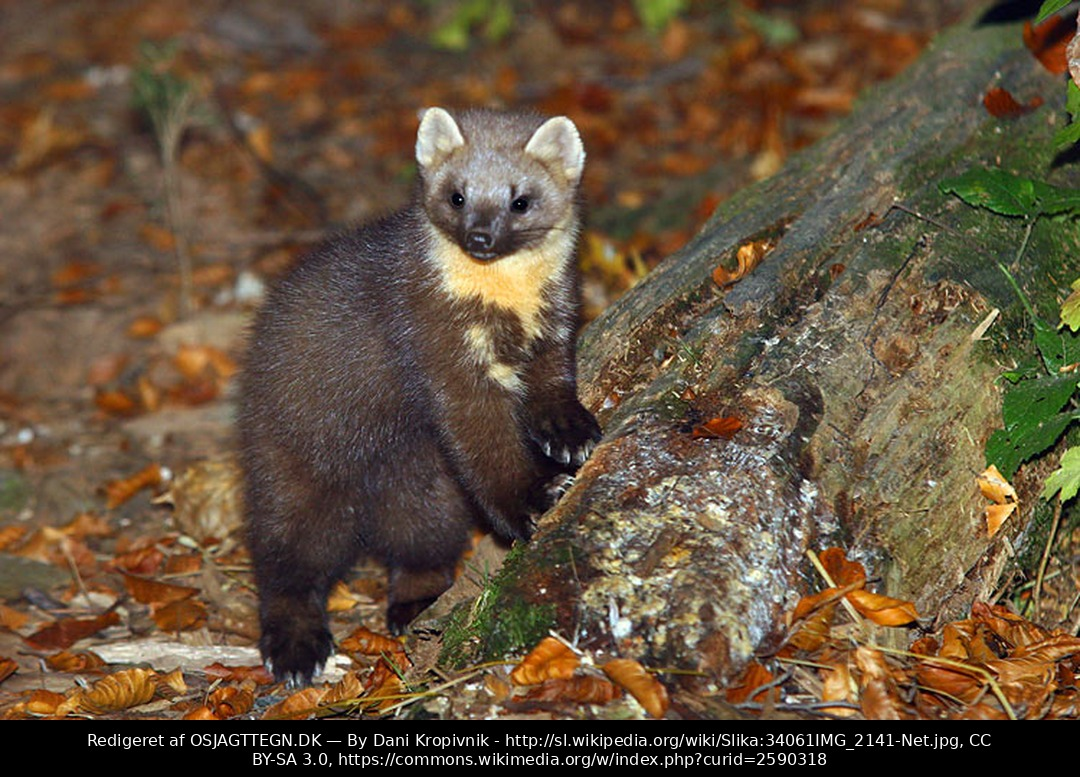
\includegraphics[width=\linewidth, height=7.2cm, keepaspectratio]{Billeder/Dyr/Pattedyr/rovdyr/skovmår/skovmaar-01.jpg}
  \end{columns}
\end{frame}

% ========== VASKEBJØRN ==========
\begin{frame}{%
  \begin{minipage}[c]{0.30\textwidth}
    Vaskebjørn
  \end{minipage}%
  \hfill
  \begin{minipage}[c]{0.45\textwidth}
    \footnotesize
    \textbf{Jagttid:} Hele året\\
    \textbf{Regulering:} Uden aftale (invasiv)
  \end{minipage}%
  \hfill
  \begin{minipage}[c]{0.15\textwidth}
    \noindent\raggedleft
    
\includegraphics[width=0.5cm, height=0.5cm, keepaspectratio]{Billeder/Ikoner/star.png}
  \end{minipage}%
}
  \vspace{0.25em}
  \begin{columns}[T]
    % --- Venstre kolonne: Tekst ---
    \column{0.45\textwidth}
    \setlength{\parskip}{0.4em}
    \tiny
    \RaggedRight
    \textbf{\textit{Procyon lotor}} – invasiv art med karakteristisk ansigtsmaske og stribet hale. \par
    \textbf{Udseende:}\\
    \quad – Grå pels med lange sorte og hvide dækhår \\
    \quad – Hale halvt så lang som kroppen og stribet \\
    \quad – Sort tværstribet ansigtsmaske
    % --- Højre kolonne: Større billede ---
    \column{0.52\textwidth}
    \centering
    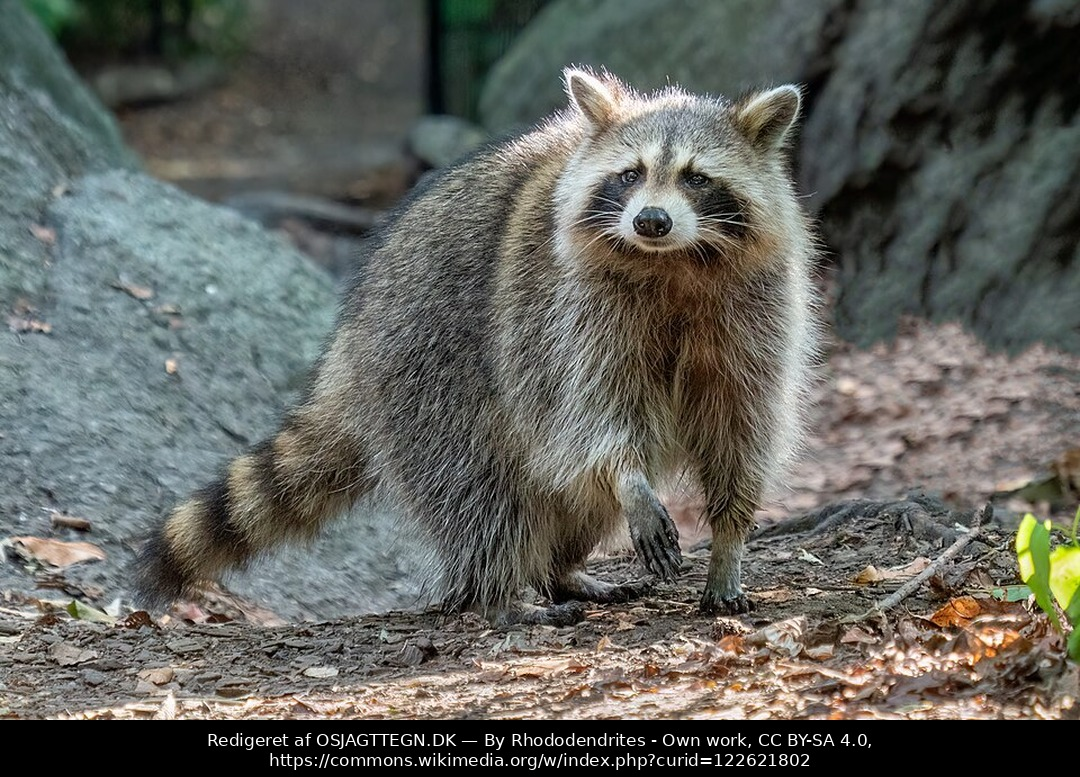
\includegraphics[width=\linewidth, height=7.2cm, keepaspectratio]{Billeder/Dyr/Pattedyr/rovdyr/vaskebjørn/vaskebjoern-01.jpg}
  \end{columns}
\end{frame}

% ========== SPÆTTET SÆL ==========
\begin{frame}{%
  \begin{minipage}[c]{0.30\textwidth}
    Spættet sæl
  \end{minipage}%
  \hfill
  \begin{minipage}[c]{0.45\textwidth}
    \footnotesize
    \textbf{Jagttid:} Ingen jagttid
  \end{minipage}%
  \hfill
  \begin{minipage}[c]{0.15\textwidth}
    \noindent\raggedleft
    
\includegraphics[width=0.5cm, height=0.5cm, keepaspectratio]{Billeder/Ikoner/star.png}
  \end{minipage}%
}
  \vspace{0.25em}
  \begin{columns}[T]
    % --- Venstre kolonne: Tekst ---
    \column{0.45\textwidth}
    \setlength{\parskip}{0.4em}
    \tiny
    \RaggedRight
    \textbf{\textit{Phoca vitulina}} – den almindeligste sæl i Danmark. \par
    \textbf{Udseende:}\\
    \quad – Pelsen varierer, oftest med sorte eller grålige pletter \\
    \quad – Kendes på V-formede næsebor
    % --- Højre kolonne: Større billede ---
    \column{0.52\textwidth}
    \centering
    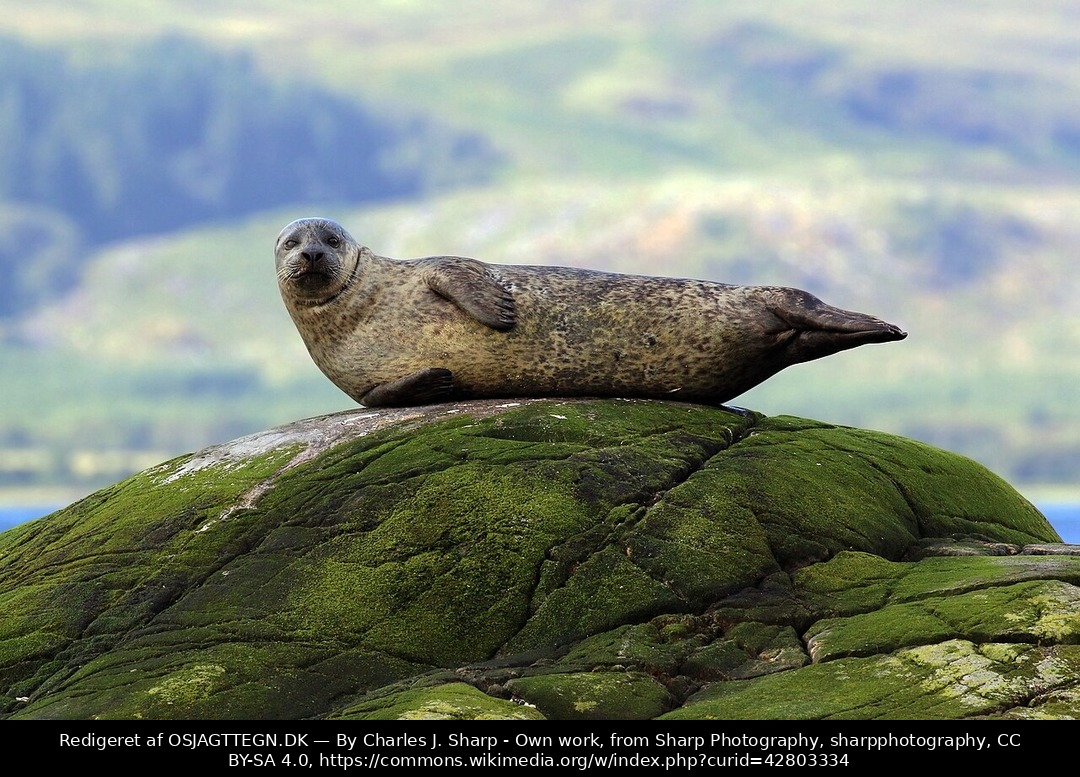
\includegraphics[width=\linewidth, height=7.2cm, keepaspectratio]{Billeder/Dyr/Pattedyr/rovdyr/spættet_sæl/spaettetsael-01.jpg}
  \end{columns}
\end{frame}

% ========== GRÅSÆL ==========
\begin{frame}{%
  \begin{minipage}[c]{0.30\textwidth}
    Gråsæl
  \end{minipage}%
  \hfill
  \begin{minipage}[c]{0.45\textwidth}
    \footnotesize
    \textbf{Jagttid:} Ingen jagttid
  \end{minipage}%
  \hfill
  \begin{minipage}[c]{0.15\textwidth}
    \noindent\raggedleft
    
\includegraphics[width=0.5cm, height=0.5cm, keepaspectratio]{Billeder/Ikoner/star.png}
  \end{minipage}%
}
  \vspace{0.25em}
  \begin{columns}[T]
    % --- Venstre kolonne: Tekst ---
    \column{0.45\textwidth}
    \setlength{\parskip}{0.4em}
    \tiny
    \RaggedRight
    \textbf{\textit{Halichoerus grypus}} – større end spættet sæl og med mere langstrakt hoved. \par
    \textbf{Udseende:}\\
    \quad – Grålig pels \\
    \quad – Næseborene er parallelle, modsat den spættede sæl
    % --- Højre kolonne: Større billede ---
    \column{0.52\textwidth}
    \centering
    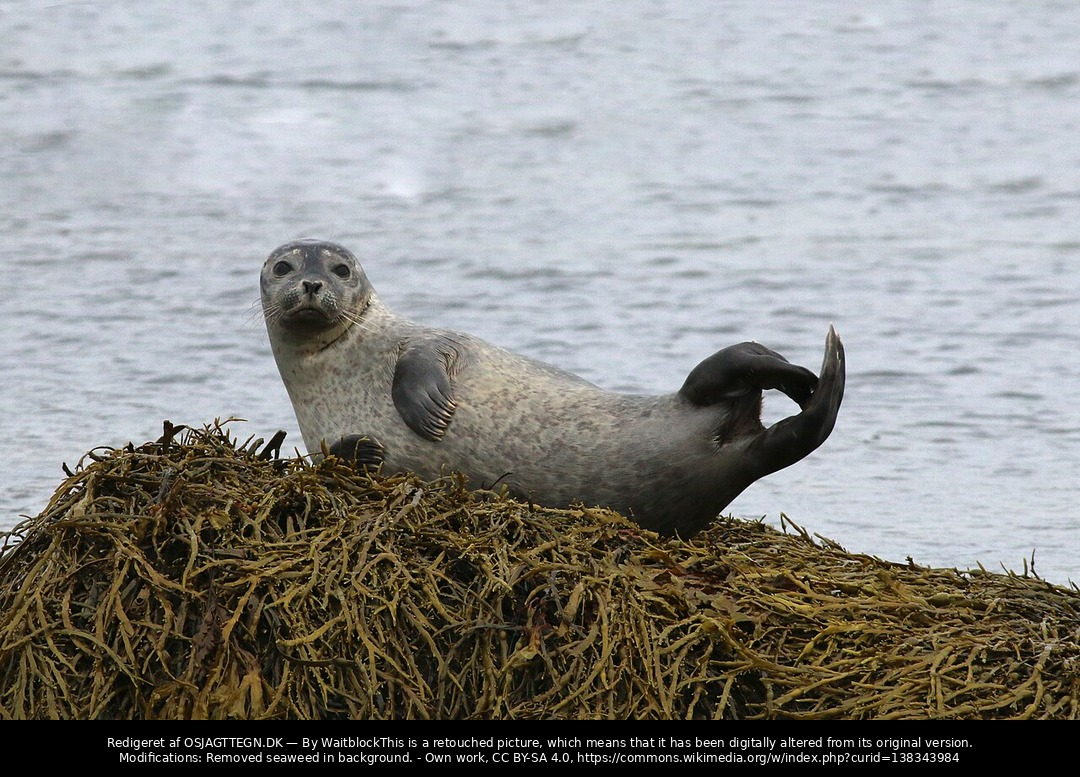
\includegraphics[width=\linewidth, height=7.2cm, keepaspectratio]{Billeder/Dyr/Pattedyr/rovdyr/gråsæl/graasael-02.jpg}
  \end{columns}
\end{frame}

\begin{frame}
  \vspace{1.8em}
  \begin{center}
    \begin{minipage}{0.22\textwidth}
      \centering
      
\includegraphics[width=\linewidth]{Billeder/Dyr/Pattedyr/rovdyr/rovdyr_qr/rovdyr_qrcode.png}
    \end{minipage}%
    \hspace{0.8em}%
    \begin{minipage}{0.62\textwidth}
      \raggedright
      \Large
      \textbf{Træning i artsbestemmelse af rovdyr}\\[0.35em]
      {\large https://osjagttegn.dk/rovdyr}
    \end{minipage}
  \end{center}
\end{frame}
\section{Gnavere og støttetandede (Artsbestemmeæse \& biologi)}

% ========== TITEL: GNAVERE OG STØTTETANDEDE ==========
\begin{frame}
  \vspace{1.5em}
  \begin{center}
    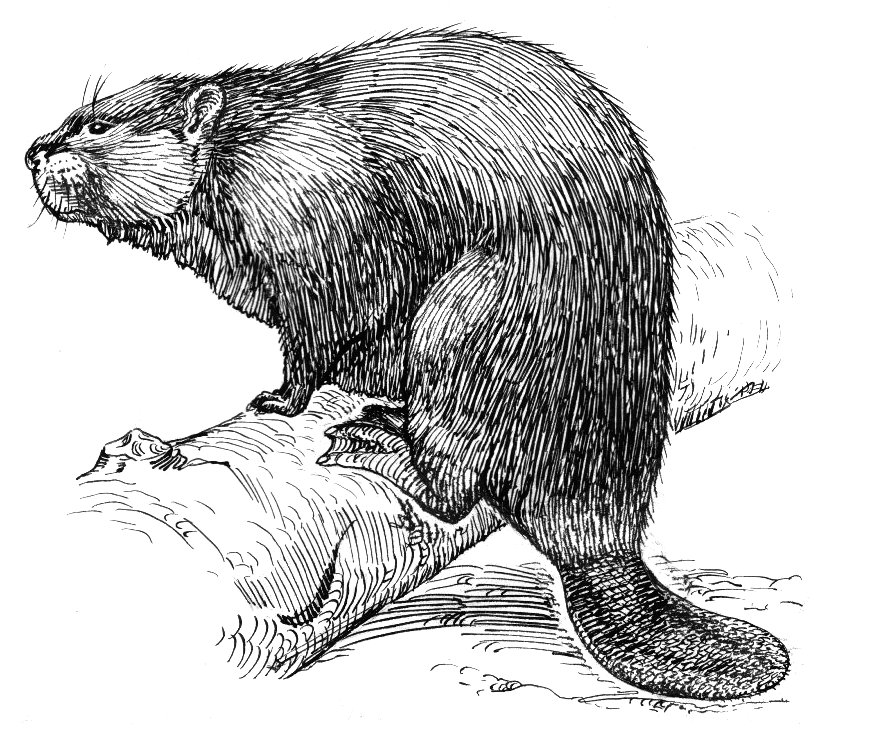
\includegraphics[width=12cm, height=4cm, keepaspectratio]{Billeder/Dyr/Pattedyr/støttetandede/gnaver.jpg}\\[1.2em]
    {\LARGE \textbf{Gnavere og støttetandede}}\\[0.6em]
    
    Artsbestemmelse \& vildtbiologi  \\[0.9em]
    {\tiny\color{gray}
    CC BY 4.0 – kan frit anvendes, også kommercielt. Rettighederne må ikke skærpes.\\[0.05em]
    Udviklet af Aleksander Sønder, OSJAGTTEGN.DK}
  \end{center}
\end{frame}

% ========== HARE ==========
\begin{frame}{%
  \begin{minipage}[c]{0.30\textwidth}
    Hare
  \end{minipage}%
  \hfill
  \begin{minipage}[c]{0.45\textwidth}
    \footnotesize
    \textbf{Jagttid:} 1.\ oktober -- 31.\ januar
  \end{minipage}%
  \hfill
  \begin{minipage}[c]{0.15\textwidth}
    \noindent\raggedleft
    
\includegraphics[width=0.5cm, height=0.5cm, keepaspectratio]{Billeder/Ikoner/star.png}%
    \hspace{0.2em}%
    
\includegraphics[width=0.5cm, height=0.5cm, keepaspectratio]{Billeder/Ikoner/star.png}%
    \hspace{0.2em}%
    
\includegraphics[width=0.5cm, height=0.5cm, keepaspectratio]{Billeder/Ikoner/star.png}
  \end{minipage}%
}
  \vspace{0.25em}
  \begin{columns}[T]
    % --- Venstre kolonne: Tekst ---
    \column{0.45\textwidth}
    \setlength{\parskip}{0.4em}
    \tiny
    \RaggedRight
    \textbf{\textit{Lepus europaeus}} – kendes på de meget lange ører og lange ben. \par
    \textbf{Udseende:}\\
    \quad – Lange ører med sorte spidser \\
    \quad – Gråbrun pels \\
    \quad – Bagben længere end forbenene \par
    \textbf{Levesteder:} Knyttet til det åbne land, men findes også i skovområder. \par
    \textbf{Føde:} Friske skud af græs og urter samt landbrugsafgrøder. Pseudo-drøvtygger. \par
    \textbf{Udbredelse:} Hele landet. \par
    \textbf{Parring/brunst:} Januar--september. \par
    \textbf{Forplantning:}\\
    \quad – \textbf{Kønsmoden:} 1 år \\
    \quad – \textbf{Mono/polygam:} Polygam \\
    \quad – \textbf{Bestandsomsætning:} Hurtig \\
    \quad – \textbf{Kuld:} 2--4 kuld med 2--4 killinger pr.\ kuld \par
    % --- Højre kolonne: Større billede ---
    \column{0.52\textwidth}
    \centering
    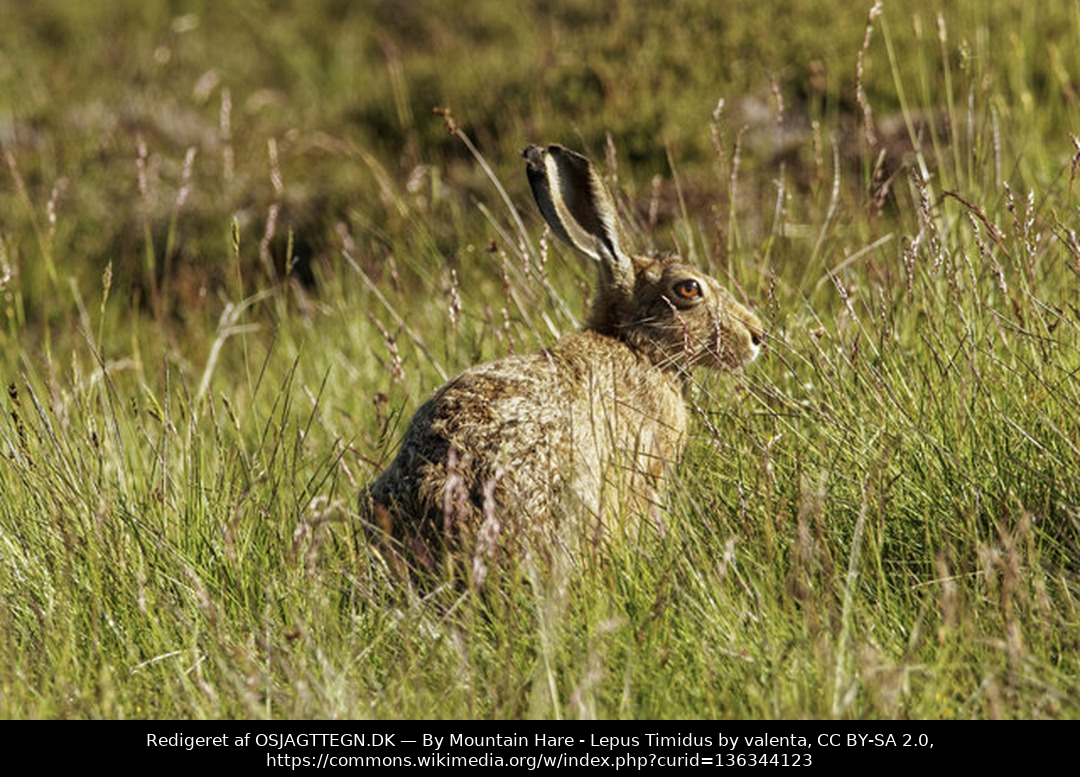
\includegraphics[width=\linewidth, height=7.2cm, keepaspectratio]{Billeder/Dyr/Pattedyr/støttetandede/hare/hare-04.jpg}
  \end{columns}
\end{frame}

% ========== VILDKANIN ==========
\begin{frame}{%
  \begin{minipage}[c]{0.30\textwidth}
    Vildkanin
  \end{minipage}%
  \hfill
  \begin{minipage}[c]{0.45\textwidth}
    \footnotesize
    \textbf{Jagttid:} 1.\ september -- 31.\ januar
  \end{minipage}%
  \hfill
  \begin{minipage}[c]{0.15\textwidth}
    \noindent\raggedleft
    
\includegraphics[width=0.5cm, height=0.5cm, keepaspectratio]{Billeder/Ikoner/star.png}%
    \hspace{0.2em}%
    
\includegraphics[width=0.5cm, height=0.5cm, keepaspectratio]{Billeder/Ikoner/star.png}
  \end{minipage}%
}
  \vspace{0.25em}
  \begin{columns}[T]
    % --- Venstre kolonne: Tekst ---
    \column{0.45\textwidth}
    \setlength{\parskip}{0.4em}
    \tiny
    \RaggedRight
    \textbf{\textit{Oryctolagus cuniculus}} – forholdsvis lange ører, men mere kompakt end haren. \par
    \textbf{Udseende:}\\
    \quad – Benene næsten lige lange \\
    \quad – Brun overside \\
    \quad – Hvid underside \par
    \textbf{Levesteder:} I kolonier under jorden nær åbne arealer. \par
    \textbf{Føde:} Friske skud af græsser og urter samt markafgrøder. Pseudo-drøvtygger. \par
    \textbf{Udbredelse:} Sønderjylland, Fanø, Als, Endelave og Bornholm.
    % --- Højre kolonne: Større billede ---
    \column{0.52\textwidth}
    \centering
    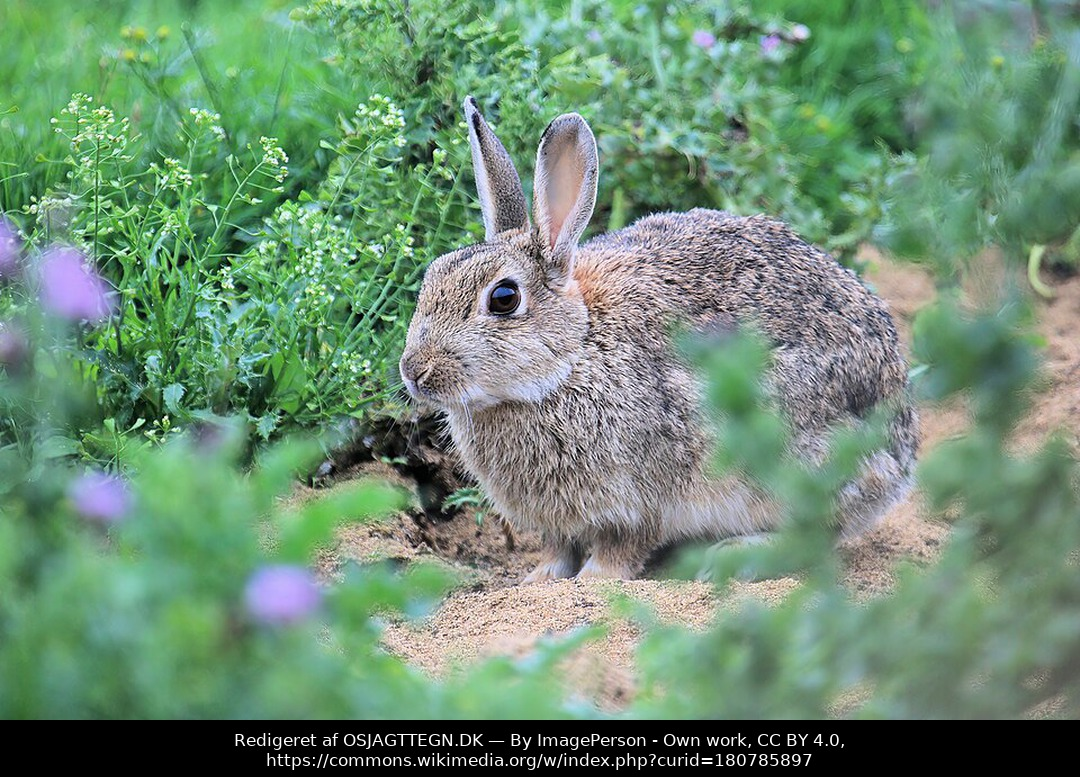
\includegraphics[width=\linewidth, height=7.2cm, keepaspectratio]{Billeder/Dyr/Pattedyr/støttetandede/vildkanin/vildkanin-02.jpg}
  \end{columns}
\end{frame}

% ========== EGERN ==========
\begin{frame}{%
  \begin{minipage}[c]{0.30\textwidth}
    Egern
  \end{minipage}%
  \hfill
  \begin{minipage}[c]{0.45\textwidth}
    \footnotesize
    \textbf{Jagttid:} Ingen jagttid
  \end{minipage}%
  \hfill
  \begin{minipage}[c]{0.15\textwidth}
    \noindent\raggedleft
    
\includegraphics[width=0.5cm, height=0.5cm, keepaspectratio]{Billeder/Ikoner/star.png}
  \end{minipage}%
}
  \vspace{0.25em}
  \begin{columns}[T]
    % --- Venstre kolonne: Tekst ---
    \column{0.45\textwidth}
    \setlength{\parskip}{0.4em}
    \tiny
    \RaggedRight
    \textbf{\textit{Sciurus vulgaris}} – lille gnaver med busket hale. \par
    \textbf{Udseende:}\\
    \quad – Pelsfarven varierer fra rød over brun til næsten sort \\
    \quad – Undersiden er som regel hvid
    % --- Højre kolonne: Større billede ---
    \column{0.52\textwidth}
    \centering
    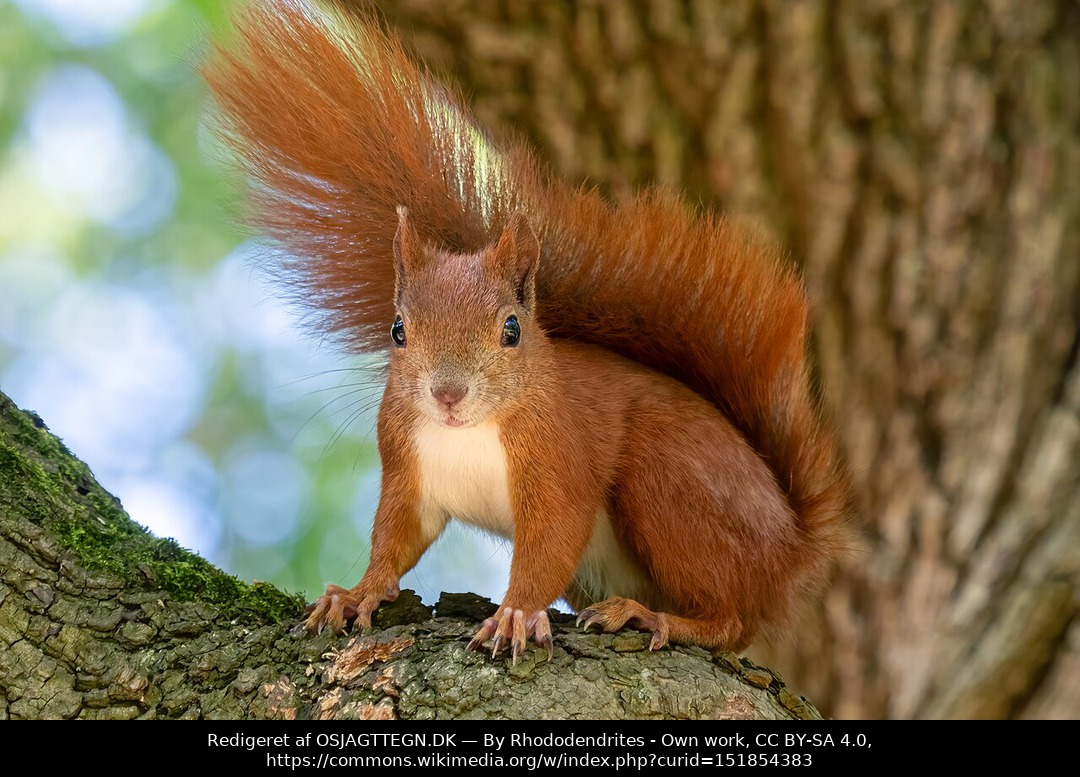
\includegraphics[width=\linewidth, height=7.2cm, keepaspectratio]{Billeder/Dyr/Pattedyr/støttetandede/egern/egern-01.jpg}
  \end{columns}
\end{frame}

% ========== BÆVER ==========
\begin{frame}{%
  \begin{minipage}[c]{0.30\textwidth}
    Bæver
  \end{minipage}%
  \hfill
  \begin{minipage}[c]{0.45\textwidth}
    \footnotesize
    \textbf{Jagttid:} Ingen jagttid
  \end{minipage}%
  \hfill
  \begin{minipage}[c]{0.15\textwidth}
    \noindent\raggedleft
    
\includegraphics[width=0.5cm, height=0.5cm, keepaspectratio]{Billeder/Ikoner/star.png}
  \end{minipage}%
}
  \vspace{0.25em}
  \begin{columns}[T]
    % --- Venstre kolonne: Tekst ---
    \column{0.45\textwidth}
    \setlength{\parskip}{0.4em}
    \tiny
    \RaggedRight
    \textbf{\textit{Castor fiber}} – stor gnaver knyttet til vandløb og søer. \par
    \textbf{Udseende:}\\
    \quad – Ensfarvet pels med lange, stride hår \\
    \quad – Bred, nøgen hale med skællet hud \\
    \quad – Lange, skarpe fortænder
    % --- Højre kolonne: Større billede ---
    \column{0.52\textwidth}
    \centering
    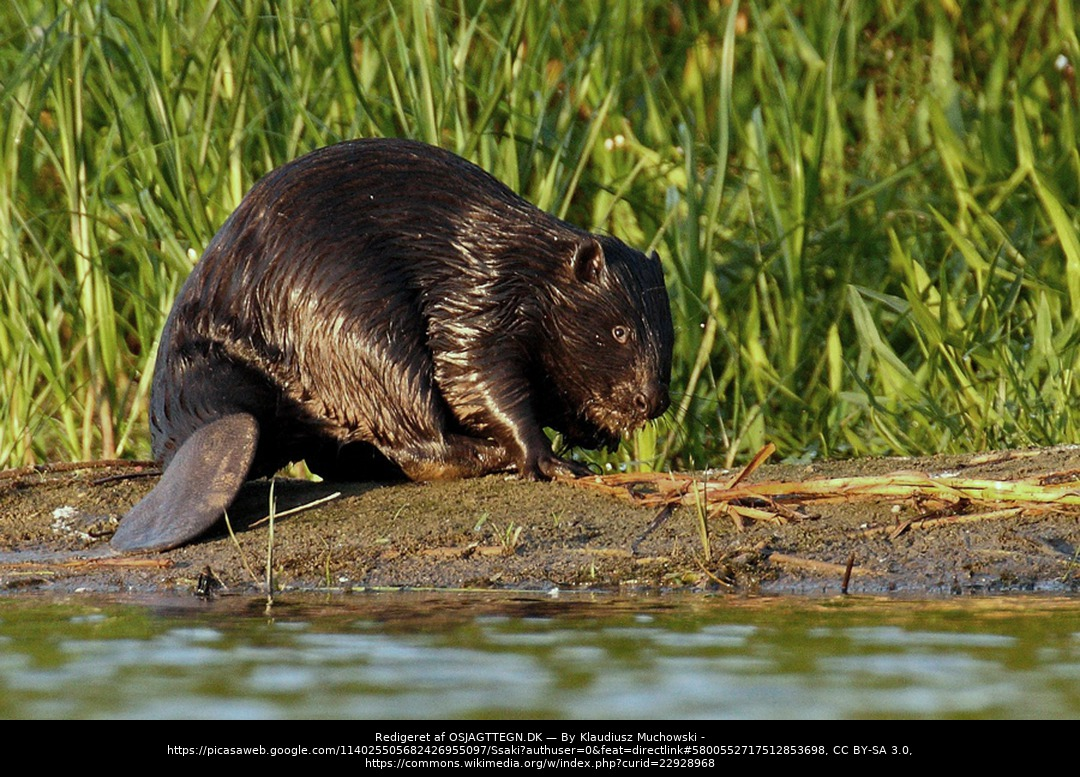
\includegraphics[width=\linewidth, height=7.2cm, keepaspectratio]{Billeder/Dyr/Pattedyr/støttetandede/bæver/baever-01.jpg}
  \end{columns}
\end{frame}

% ========== SUMPBÆVER ==========
\begin{frame}{%
  \begin{minipage}[c]{0.30\textwidth}
    Sumpbæver
  \end{minipage}%
  \hfill
  \begin{minipage}[c]{0.45\textwidth}
    \footnotesize
    \textbf{Jagttid:} Hele året\\
    \textbf{Regulering:} Uden aftale (invasiv)
  \end{minipage}%
  \hfill
  \begin{minipage}[c]{0.15\textwidth}
    \noindent\raggedleft
    
\includegraphics[width=0.5cm, height=0.5cm, keepaspectratio]{Billeder/Ikoner/star.png}
  \end{minipage}%
}
  \vspace{0.25em}
  \begin{columns}[T]
    % --- Venstre kolonne: Tekst ---
    \column{0.45\textwidth}
    \setlength{\parskip}{0.4em}
    \tiny
    \RaggedRight
    \textbf{\textit{Myocastor coypus}} – invasiv gnaver knyttet til vådområder. \par
    \textbf{Udseende:}\\
    \quad – Grov, brunlig pels \\
    \quad – Stort hoved i forhold til kroppen \\
    \quad – Rund, skællet hale med få hår
    % --- Højre kolonne: Større billede ---
    \column{0.52\textwidth}
    \centering
    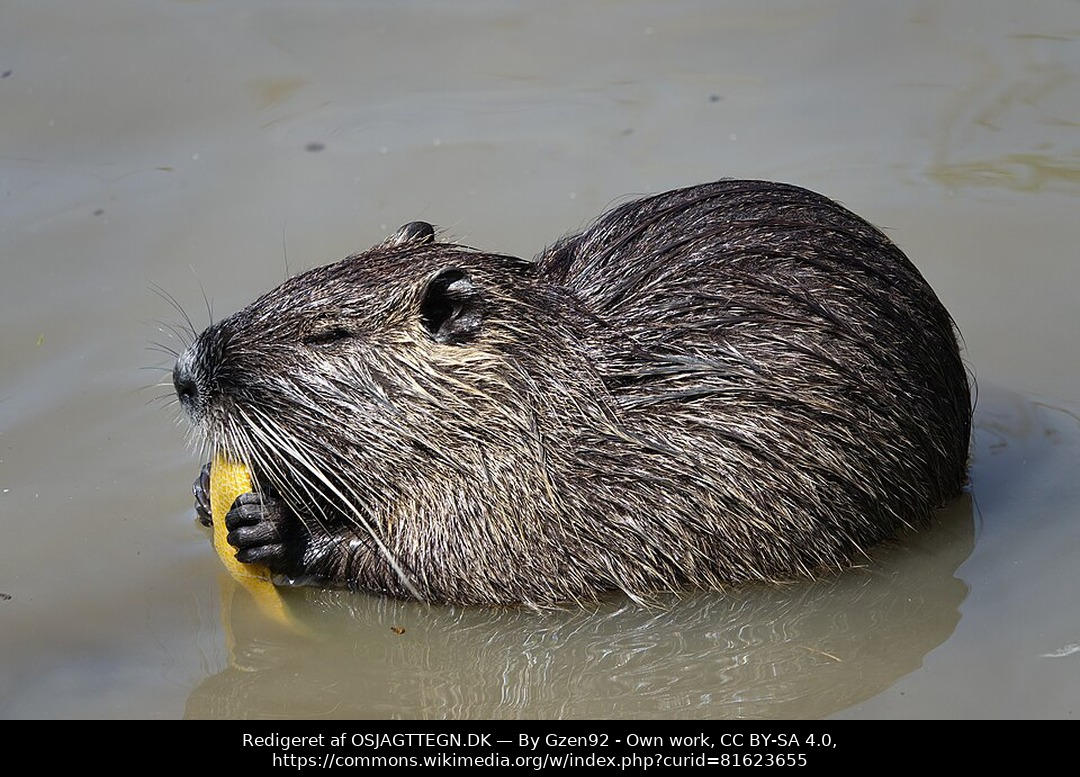
\includegraphics[width=\linewidth, height=7.2cm, keepaspectratio]{Billeder/Dyr/Pattedyr/støttetandede/sumpbæver/sumpbaever-01.jpg}
  \end{columns}
\end{frame}

% ========== BISAMROTTE ==========
\begin{frame}{%
  \begin{minipage}[c]{0.30\textwidth}
    Bisamrotte
  \end{minipage}%
  \hfill
  \begin{minipage}[c]{0.45\textwidth}
    \footnotesize
    \textbf{Jagttid:} Hele året\\
    \textbf{Regulering:} Uden aftale (invasiv)
  \end{minipage}%
  \hfill
  \begin{minipage}[c]{0.15\textwidth}
    \noindent\raggedleft
    
\includegraphics[width=0.5cm, height=0.5cm, keepaspectratio]{Billeder/Ikoner/star.png}
  \end{minipage}%
}
  \vspace{0.25em}
  \begin{columns}[T]
    % --- Venstre kolonne: Tekst ---
    \column{0.45\textwidth}
    \setlength{\parskip}{0.4em}
    \tiny
    \RaggedRight
    \textbf{\textit{Ondatra zibethicus}} – invasiv gnaver knyttet til søer, åer og moser. \par
    \textbf{Udseende:}\\
    \quad – Brunlig og buttet med kort snude \\
    \quad – Hale med skællet hud og få hår
    % --- Højre kolonne: Større billede ---
    \column{0.52\textwidth}
    \centering
    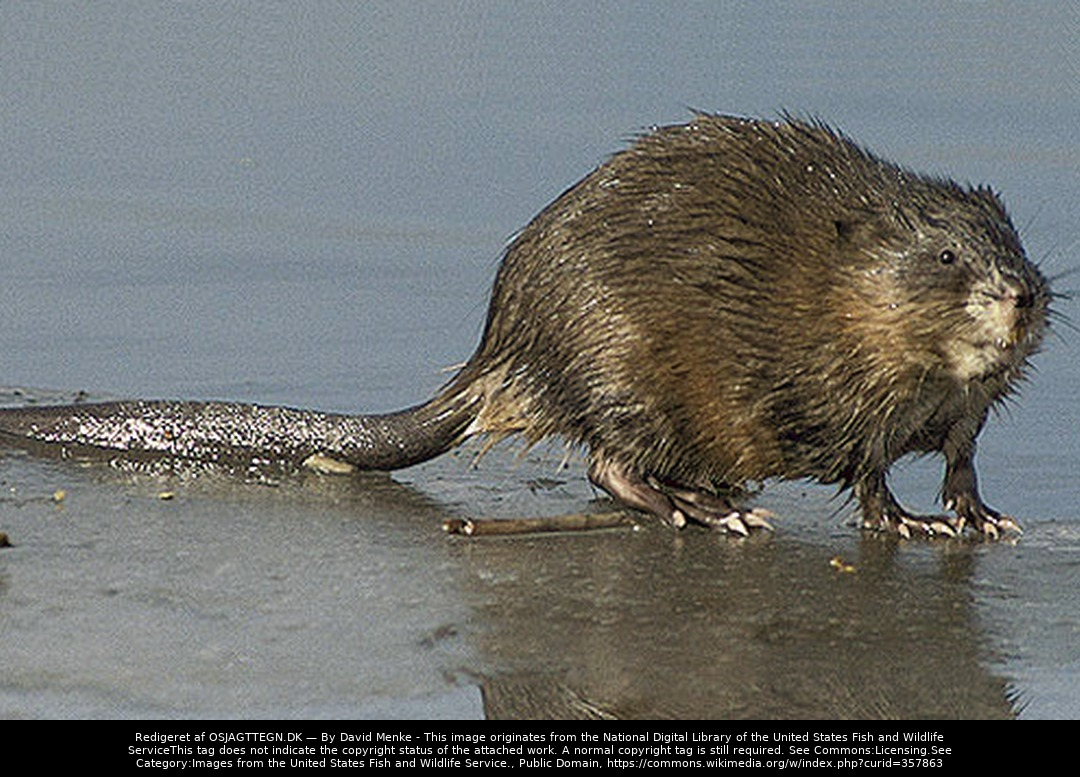
\includegraphics[width=\linewidth, height=7.2cm, keepaspectratio]{Billeder/Dyr/Pattedyr/støttetandede/bisamrotte/bisamrotte-01.jpg}
  \end{columns}
\end{frame}

\begin{frame}
  \vspace{1.8em}
  \begin{center}
    \begin{minipage}{0.22\textwidth}
      \centering
      
\includegraphics[width=\linewidth]{Billeder/Dyr/Pattedyr/støttetandede/qr_støtte.png}
    \end{minipage}%
    \hspace{0.8em}%
    \begin{minipage}{0.62\textwidth}
      \raggedright
      \Large
      \textbf{Træning i artsbestemmelse af gnavere og støttetandende}\\[0.35em]
      {\large https://osjagttegn.dk/gnavere-og-stoettetandede}
    \end{minipage}
  \end{center}
\end{frame}
\section{Jagtetiske regler for kronvildt}

\begin{frame}
  \vspace{3em}
  \begin{center}
    {\LARGE \textbf{Jagtetiske regler for kronvildt}
    }
    \\
    \vspace{1em}
    Vildtforvaltningsrådet \\
    https://sgavmst.dk/media/vcupseet/de-jagtetiske-regler-for-kronvildt.pdf
  \end{center}
\end{frame}

\begin{frame}{Formål \& Ansvar}
\begin{itemize}
\item Sikre bred offentlig accept af kronvildtjagt – grundlag for fortsat jagt uden stramme restriktioner
\item Regler udarbejdet af Vildtforvaltningsrådet
\item Den enkelte jægers ansvar: Værne om kronvildt og jagten ved at følge reglerne
\item Fokus: Naturlig bestand, nabohensyn, bæredygtighed, ren skydning og minimal forstyrrelse
\end{itemize}
\end{frame}

\begin{frame}{Afskydningspolitik}
\begin{itemize}
\item Tilrettelæg afskydning for naturlig køns- og aldersfordeling
\item Størst afskydning blandt unge dyr (kalve + unghjorte/unghinder)
\item Jævn fordeling mellem handyr og hundyr
\item Indskrænk septemberjagten på hjorte mest muligt → giver ro i brunsten
\item Undgå ubalance (mange hjorte – få hinder/kalve)
\end{itemize}
\end{frame}

\begin{frame}{Nabohensyn \& Terrænstørrelse}
\begin{itemize}
\item Afskydning skal stå i rimeligt forhold til terrænets størrelse
\item Sigt mod at vildt falder på eget område (kronvildt går ofte 100 m+)
\item Ikke flere end 1 stk. pr. sæson på arealer mindre end 25 ha
\item På små/smalle arealer: Indgå naboaftaler eller fælles jagt/forståelse
\item Skel mellem kerneområder (sædvanlig ophold) og vandringsområder
\end{itemize}
\end{frame}

\begin{frame}{Bæredygtig jagtudnyttelse}
\begin{itemize}
\item Bæredygtighed vurderes lokalt – ikke nationalt
\item Typisk max 1 stk. pr. 25–50 ha pr. sæson (lavere på større ejendomme)
\item Kerneområder (ro, dækning, føde) tåler højere afskydning pr. ha
\item Yderområder: Lavere afskydning for at etablere fast bestand
\item Kronvildt har store revirer → elastisk bæredygtighedsbegreb
\end{itemize}
\end{frame}

\begin{frame}{Skydning \& Skydefærdigheder}
\begin{itemize}
\item Vær sikker på, hvad du skyder på – hold hovedet koldt ved dyr i rudel
\item Foretræk sideskud – skyd helst på dyr i ro
\item Ingen chancebetonede skud – træn på skive + bevægeligt mål
\item Kend dine begrænsninger – træn også luftbøsse/bevægelige mål/tørtræning
\item Brug hochsitz/hochstand når muligt
\end{itemize}
\end{frame}

\begin{frame}{Anskydninger \& Eftersøgning}
\begin{itemize}
\item Vær meget opmærksom på skudtegn
\item Skyd ikke til friskt dyr, hvis tidligere skudt dyr ikke ligger synligt forendt
\item Brug altid schweisshund ved tvivl/anskydning
\item Afmærk præcist ved tvivl – tilkald erfaren schweisshundefører
\item Hjælp hundefører med gode observationer – undgå flere skud i samme område
\item Mål: Minimal antal anskydninger – skylder vi kronvildtet og hinanden
\end{itemize}
\end{frame}

\begin{frame}{Jagtudøvelse \& Forstyrrelser}
\begin{itemize}
\item Ingen tryk-/drivjagter i september (brunsten)
\item Skyd ikke diegivende hinder i oktober (kalve dier stadig)
\item Min. 3 uger mellem tryk-/drivjagter
\item Max 3–4 fællesjagter pr. sæson på samme revir
\item Begræns hurtigtgående store hunde til drivjagt
\item Pürsch foretrækkes – undgå simultan pürsch over hele terræn
\item Frihold områder under fællesjagter – kronvildt kræver ro (især i etableringsfase)
\end{itemize}
\end{frame}

\begin{frame}{Dialog \& Regionale Krondyrgrupper}
\begin{itemize}
\item Planlæg afskydning lokalt sammen med naboer/lodsejere
\item Indgå i (formelle/uformelle) samarbejder om bestand og skader
\item Bidrag til fælles ansvarsfølelse
\item Regionale Krondyrgrupper understøtter efterlevelse af reglerne
\item Bred repræsentation → bedre dialog og forvaltning
\end{itemize}

\bigskip
\textbf{Sammenfatning: Kronvildtjagt kræver særligt hensyn – forvaltes med respekt, samarbejde og selvbegrænsning.}
\end{frame}
\section{Jagttermer del 3 (R-V)}

\begin{frame}
  \vspace{3em}
  \begin{center}
    {\LARGE \textbf{Jagttermer - Del 3}
    }
    \\
    \vspace{1em}
  \end{center}
\end{frame}

\begin{frame}{Jagttermer - Del 3 (R-V)}

\vspace{0.3em} % Mindre top-afstand

\begin{columns}[T]
    % --- Venstre kolonne: R, S ---
    \column{0.48\textwidth}
    \textbf{\large R, S}
    \setlength{\parskip}{0.1em} % Mindre afstand mellem punkter
    \scriptsize % Mindre skriftstørrelse
    \RaggedRight
    \begin{itemize}
        \item \textbf{Remise:} Småbeplantning i agerlandet, anlagt for vildtets skyld.
        \item \textbf{Revir:} Jagtterræn.
        \item \textbf{Rudel:} Flok af større hjortevildt (dog ikke råvildt).
        \item \textbf{Selektiv afskydning:} Målrettet afskydning af udvalgte enkeltdyr – fx dyr i dårlig fysisk stand, eller bestemt køns- og/eller aldersgruppe.
        \item \textbf{Skudtegn:} Den måde et stykke vildt reagerer på, når det træffes af skuddet.
        \item \textbf{Skydetårn:} Platform til riffeljagt eller buejagt.
        \item \textbf{Skydestige:} Stigekonstruktion med stol til riffeljagt eller buejagt.
        \item \textbf{Skørt:} Hårdusk omkring råens kønsåbning.
        \item \textbf{Smaldyr (Smalrå/smaldå/smalhind):} Hundyr hos hjortevildtarterne i tiden fra det er udvokset, til det sætter lam/kalv første gang.
        \item \textbf{Spidshjort:} Kronhjort/dåhjort/sikahjort med gevir, der kun består af to spidse stænger uden sprosser. Typisk hjortens første gevir.
    \end{itemize}

    % --- Højre kolonne: S, T, V ---
    \column{0.48\textwidth}
    \textbf{\large S, T, V}
    \setlength{\parskip}{0.1em} % Mindre afstand mellem punkter
    \scriptsize % Mindre skriftstørrelse
    \RaggedRight
    \begin{itemize}
        \item \textbf{Stand:} Særlig adfærd hos stående hunde, som på den måde angiver, at der er vildt i terrænet.
        \item \textbf{Standvildt:} Vildtarter, der forbliver i et bestemt område hele livet igennem.
        \item \textbf{Såt:} Afgrænset område, der afdrives samlet i forbindelse med en fællesjagt.
        \item \textbf{Trækvildt:} Vildt der er i en del af året trækker ud af landet, typisk fugle.
        \item \textbf{Veksel:} Hyppigt benyttet vildtsti.
        \item \textbf{Vildt:} Alle arter af fritlevende pattedyr og fugle. Definitionen fremgår i Lov om jagt og vildtforvaltning §2 (Jagtloven).
        \item \textbf{Vildtparade:} Afsluttende samling efter fællesjagt, hvor dagens nedlagte vildt lægges frem til og æres af jagtens deltagere.
    \end{itemize}
\end{columns}

\end{frame}
\section{Våben og ammunition til jagt}

\begin{frame}
  \vspace{3em}
  \begin{center}
    {\LARGE \textbf{Bekendtgørelse om våben og ammunition der må anvendes til jagt m.v.}} \\
    \vspace{1em}
    BEK nr 1479 af 05/12/2023 \\ §§ 1-3
  \end{center}
\end{frame}

\begin{frame}{Tilladte skydevåben til jagt og regulering (§1)}
    \begin{itemize}
        \item \textbf{Glatløbede haglgeværer}:
          \begin{itemize}
            \item Pibelængde ≥ 55 cm
            \item Højst kaliber 12
            \item Højst 2 patroner (permanent begrænsning hvis konstrueret til mere)
          \end{itemize}
        \item \textbf{Riflede våben}:
          \begin{itemize}
            \item Manuelt repeterende
            \item Ikke helautomatiske/fuldautomatiske
            \item Halvautomatiske: Højst 3 patroner (permanent begrænsning hvis mere; max 2 i magasin + 1 i kammer)
            \item Luftgeværer: Min projektildiameter ≥ 5,5 mm
          \end{itemize}
        \item \textbf{Forbudt}: Revolvere og pistoler
    \end{itemize}
\end{frame}

\begin{frame}{Jagtammunition til riflede våben}
\framesubtitle{Tilladt ammunition til jagt og regulering af vildt}

\tiny
\begin{tabular}{|c|p{2.8cm}|c|c|c|c|c|}
\hline
\textbf{Klasse} & \textbf{Vildtart} &
\textbf{\begin{tabular}{@{}c@{}}Kuglediam.\\$\geq$6 mm\\$E_{100}\geq$2000 J\end{tabular}} &
\textbf{\begin{tabular}{@{}c@{}}Kuglediam.\\$\geq$5,5 mm\\$E_{100}\geq$800 J\end{tabular}} &
\textbf{\begin{tabular}{@{}c@{}}$E_{100}$\\$\geq$175 J\end{tabular}} &
\textbf{\begin{tabular}{@{}c@{}}$E_0$\\$\geq$150 J\end{tabular}} &
\textbf{\begin{tabular}{@{}c@{}}$V_0$\\$\geq$200\\m/sek.\textsuperscript{*}\end{tabular}} \\
\hline
1 & Kronvildt, Dåvildt, Sikavildt, Muflon, Vildsvin & $\times$ & & & & \\
\hline
2 & Råvildt, Sæler & $\times$ & $\times$ & & & \\
\hline
3 & Ræv, Vaskebjørn, Mårhund, Hare, Sumpbæver, Skarv, Gæs & $\times$ & $\times$ & $\times$ & & \\
\hline
4 & Husmår, Ilder, Mink, Vildkanin, Bisamrotte, Hønsefugle, Blishøne, Ænder, Måger & $\times$ & $\times$ & $\times$ & $\times$ & \\
\hline
5 & Duer, Kragefugle, Vadefugle, Stære & $\times$ & $\times$ & $\times$ & $\times$ & $\times$ \\
\hline
\end{tabular}

\vspace{0.3em}
\begin{footnotesize}
\textsuperscript{*} Luftdrevet: kuglediam.\ $\geq$ 5,5 mm \quad
\textsuperscript{1} Fx kal.\ .243, 6,5$\times$55, .270, .308, 30-06 \quad
\textsuperscript{2} Fx kal.\ 22-250, .222, .223 \\
\textsuperscript{3} Fx kal.\ .17 Rem, .22 Hornet, .221 Rem, .17 HMR \quad
\textsuperscript{4} Fx kal.\ .22 LR
\end{footnotesize}

\end{frame}

\begin{frame}{Begrænsninger for haglgeværer}
    \begin{itemize}
        \item Må bruges på vildt i \textbf{klasse 2–5} (jf. bilag 1) – ikke på sæler
        \item Råbuk med hagl: \textbf{Ikke} 16. maj – 15. juli
        \item Kaliber < 20: Kun klasse 5-vildt
        \item Permanente begrænsninger (plug/magasin-blokering) tillader brug af større magasiner
        \item \textbf{Generelt}: Våbnet skal være i forsvarlig stand
        \item \textbf{Ikke tilladt}: Helautomatiske rifler (undt. særlige tilladelser fra Naturstyrelsen ved vildtskader)
    \end{itemize}
\end{frame}

\begin{frame}{Krav til haglpatroner i glatløbede haglgeværer}
    \begin{itemize}
        \item \textbf{Vægtfylde og udgangshastighed (V1,5)}:
          \begin{itemize}
            \item ≥ 7 g/cm³: Ingen minimumshastighedskrav
            \item ≤ 9 g/cm³: Mindst 400 m/sek
            \item > 9 g/cm³: Mindst 375 m/sek
          \end{itemize}
        \item \textbf{Maks. hagl-diameter}: 4 mm
        \item \textbf{Forbudt}: Kuglepatroner i glatløbede haglgeværer
        \item \textbf{Blyhagl – totalforbud} (fra 202X):
          \begin{itemize}
            \item Må ikke forhandles, medtages eller anvendes til jagt/regulering
            \item Må ikke medtages eller anvendes til flugtskydning (inkl. skydebaner)
          \end{itemize}
    \end{itemize}
\end{frame}

\begin{frame}{Jagtammunition til riflede våben}
    \begin{itemize}
        \item \textbf{Generelt}: Må bruges til arter i bilag 1 – minimumskrav skal overholdes
        \item \textbf{Klasse 1 \& 2 vildt} (jf. bilag 1):
          \begin{itemize}
            \item Projektilet skal være \textbf{ekspanderende} eller \textbf{fragmenterende}
          \end{itemize}
        \item \textbf{Blyindhold} ≥ 1 vægtprocent:
          \begin{itemize}
            \item Forbudt at medtage eller anvende til jagt/regulering
          \end{itemize}
        \item \textbf{Undtagelser fra blyforbuddet}:
          \begin{itemize}
            \item Randtænding-ammunition
            \item Ammunition fra luft- og fjedervåben
          \end{itemize}
        \item \textbf{Totalforbud}: Våben/ammunition i kaliber \textbf{50 BMG}
        
    \end{itemize}
\end{frame}

\begin{frame}{Maksimale skudafstande}
    \begin{itemize}
        \item Råvildt (hagl str. 1-2) max 20m
        \item Gæs, ræv (hagl str. 2-3) max 25m
        \item Ænder, fasaner, hare, duer (hagl str. 2-5) max 30m
        \item Bekkasin, snepper, agerhøns (hagl str 5-7 (max 30m)
    \end{itemize}
\end{frame}

\begin{frame}{Kend dit gevær}
    \begin{center}
        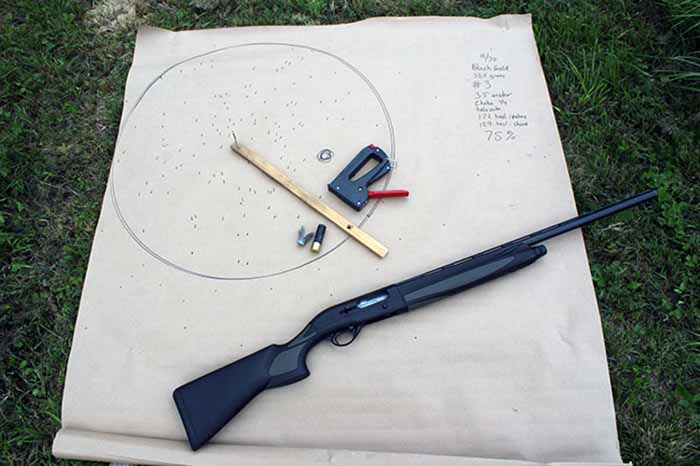
\includegraphics[width=0.7\textwidth]{Billeder/Andet/skudtest2.jpg}
        % Eller: [height=0.6\textheight] for højde-baseret skalering
    \end{center}
    
    % Her kan du tilføje tekst under billedet
    \vspace{1em}
    
\end{frame}




\begin{frame}{Jagtvåben typer}
    \begin{center}
        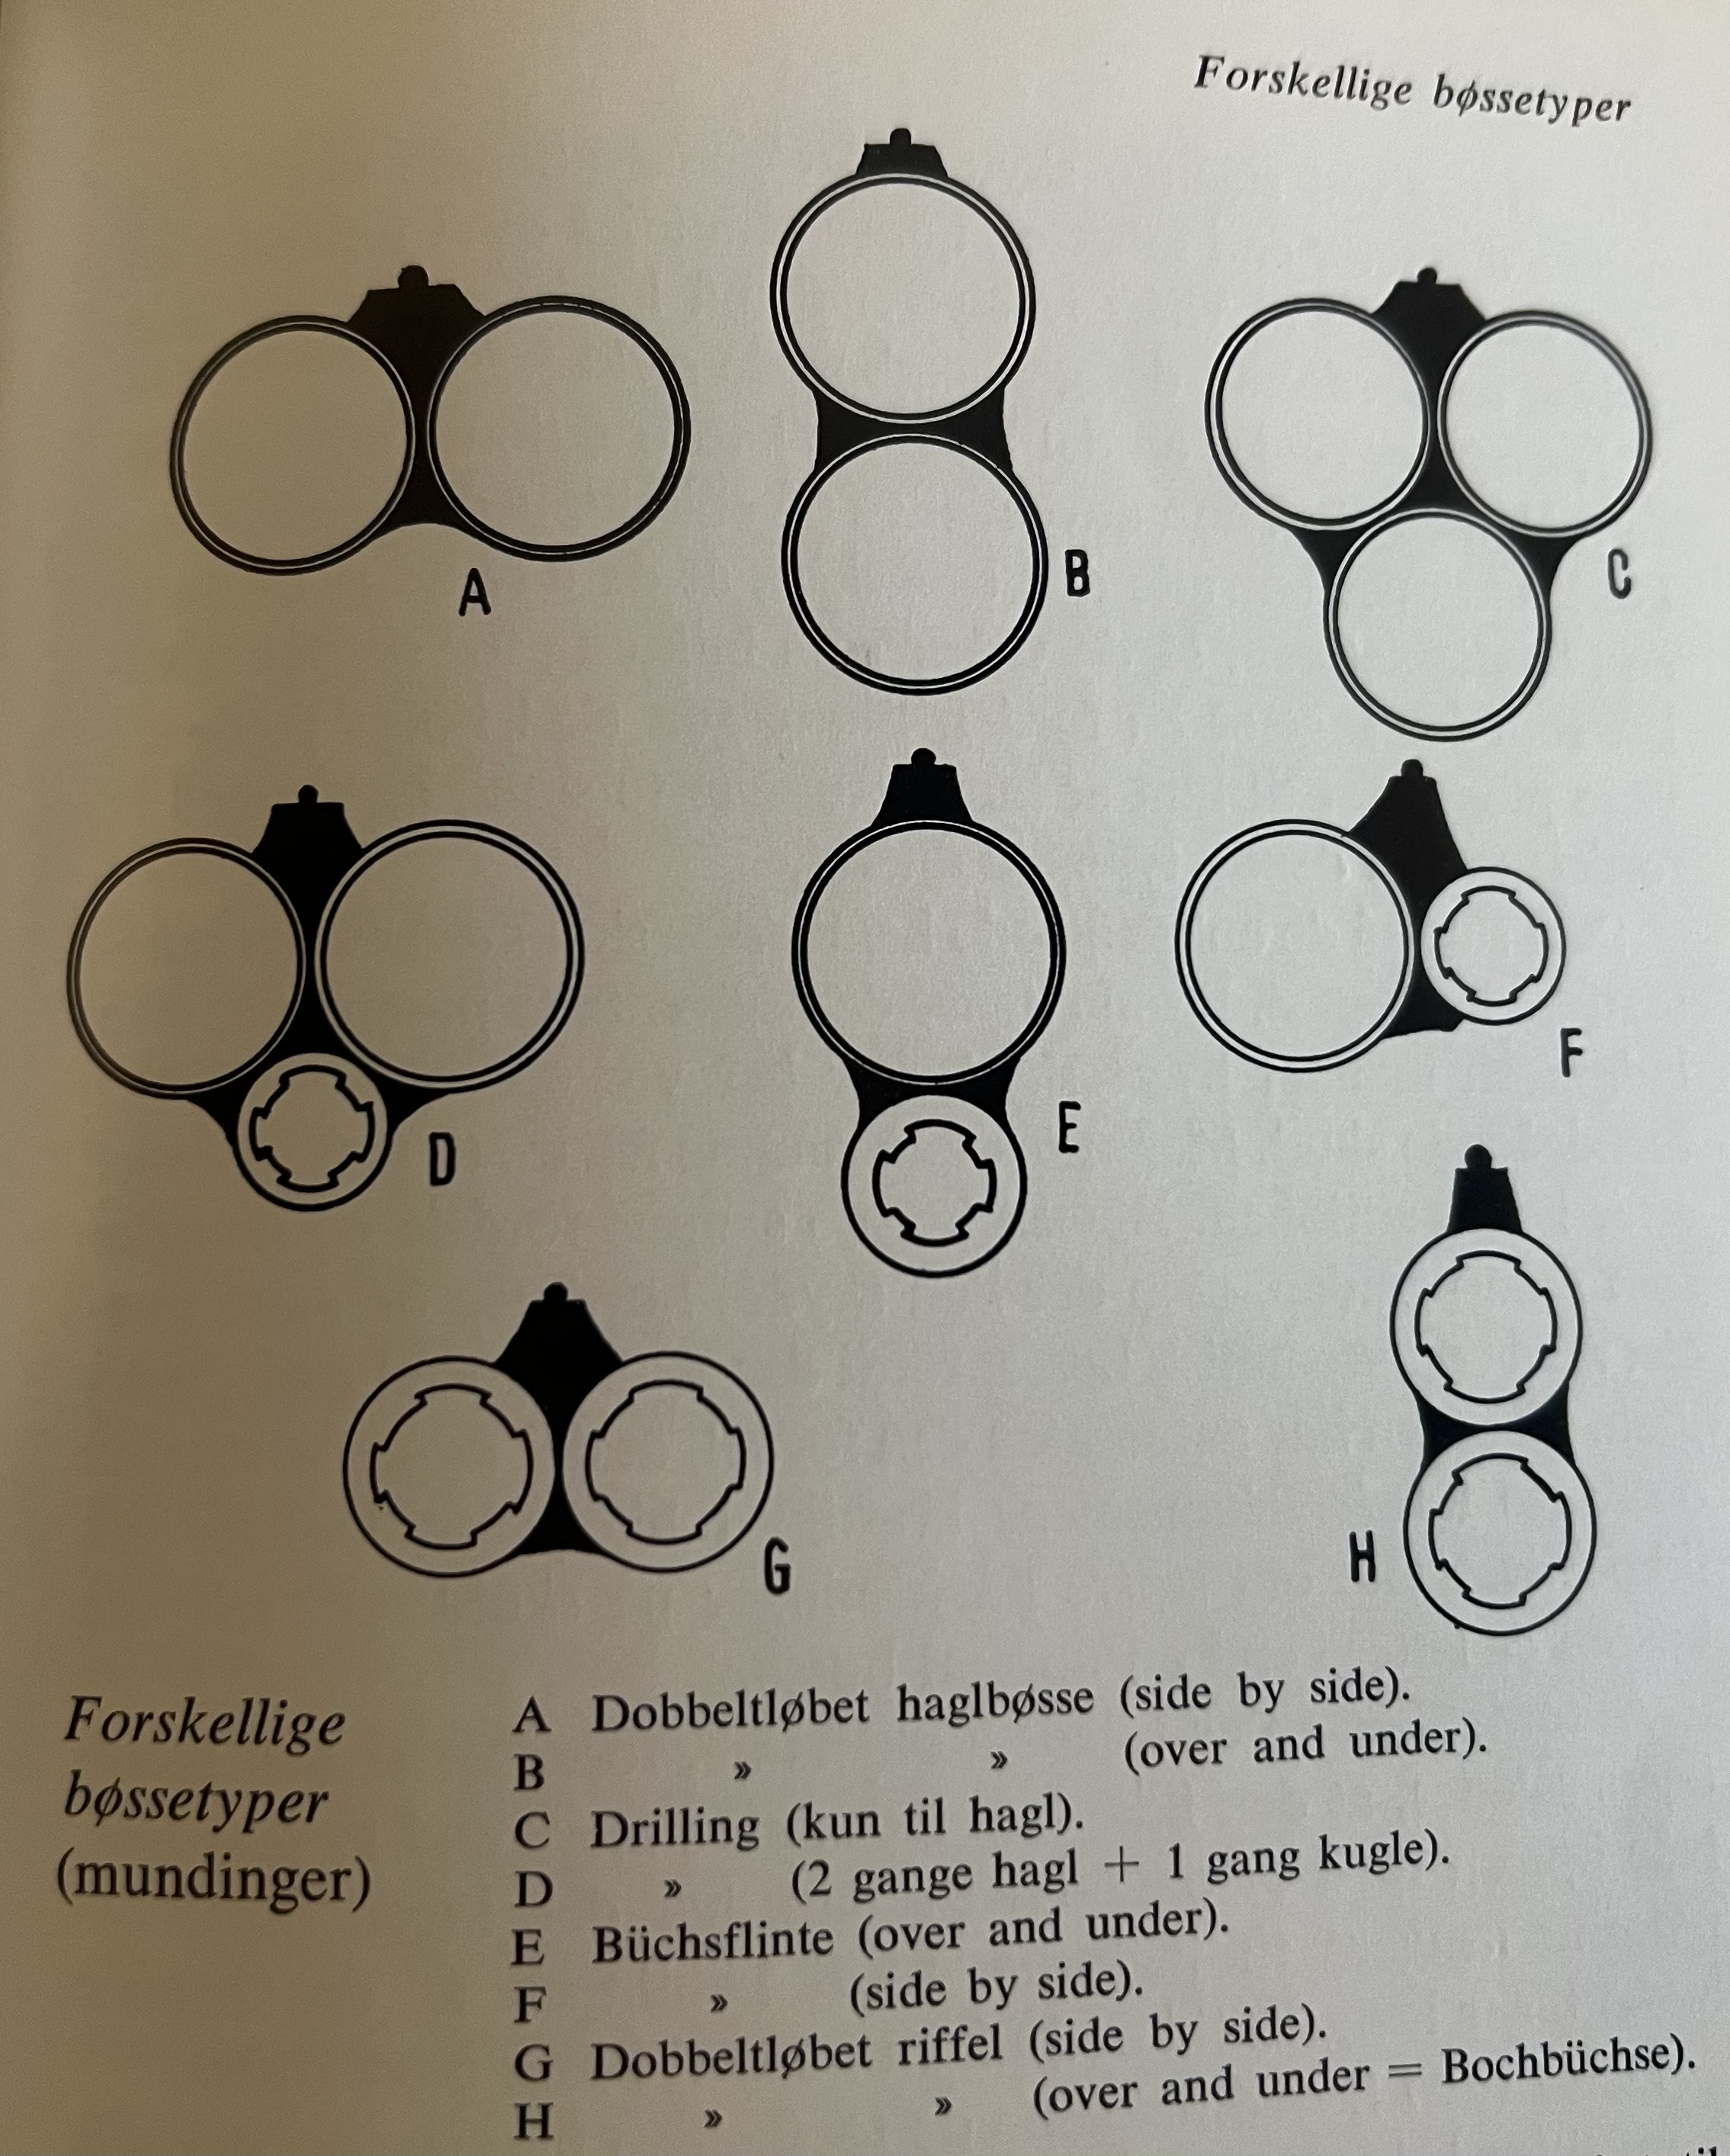
\includegraphics[width=0.3\textwidth]{Billeder/Andet/haglvarianter.jpeg}
        % Eller: [height=0.6\textheight] for højde-baseret skalering
    \end{center}
    
    % Her kan du tilføje tekst under billedet
    \vspace{1em}
    
\end{frame}

\begin{frame}{Haglvåben skæftetyper}
    \begin{center}
        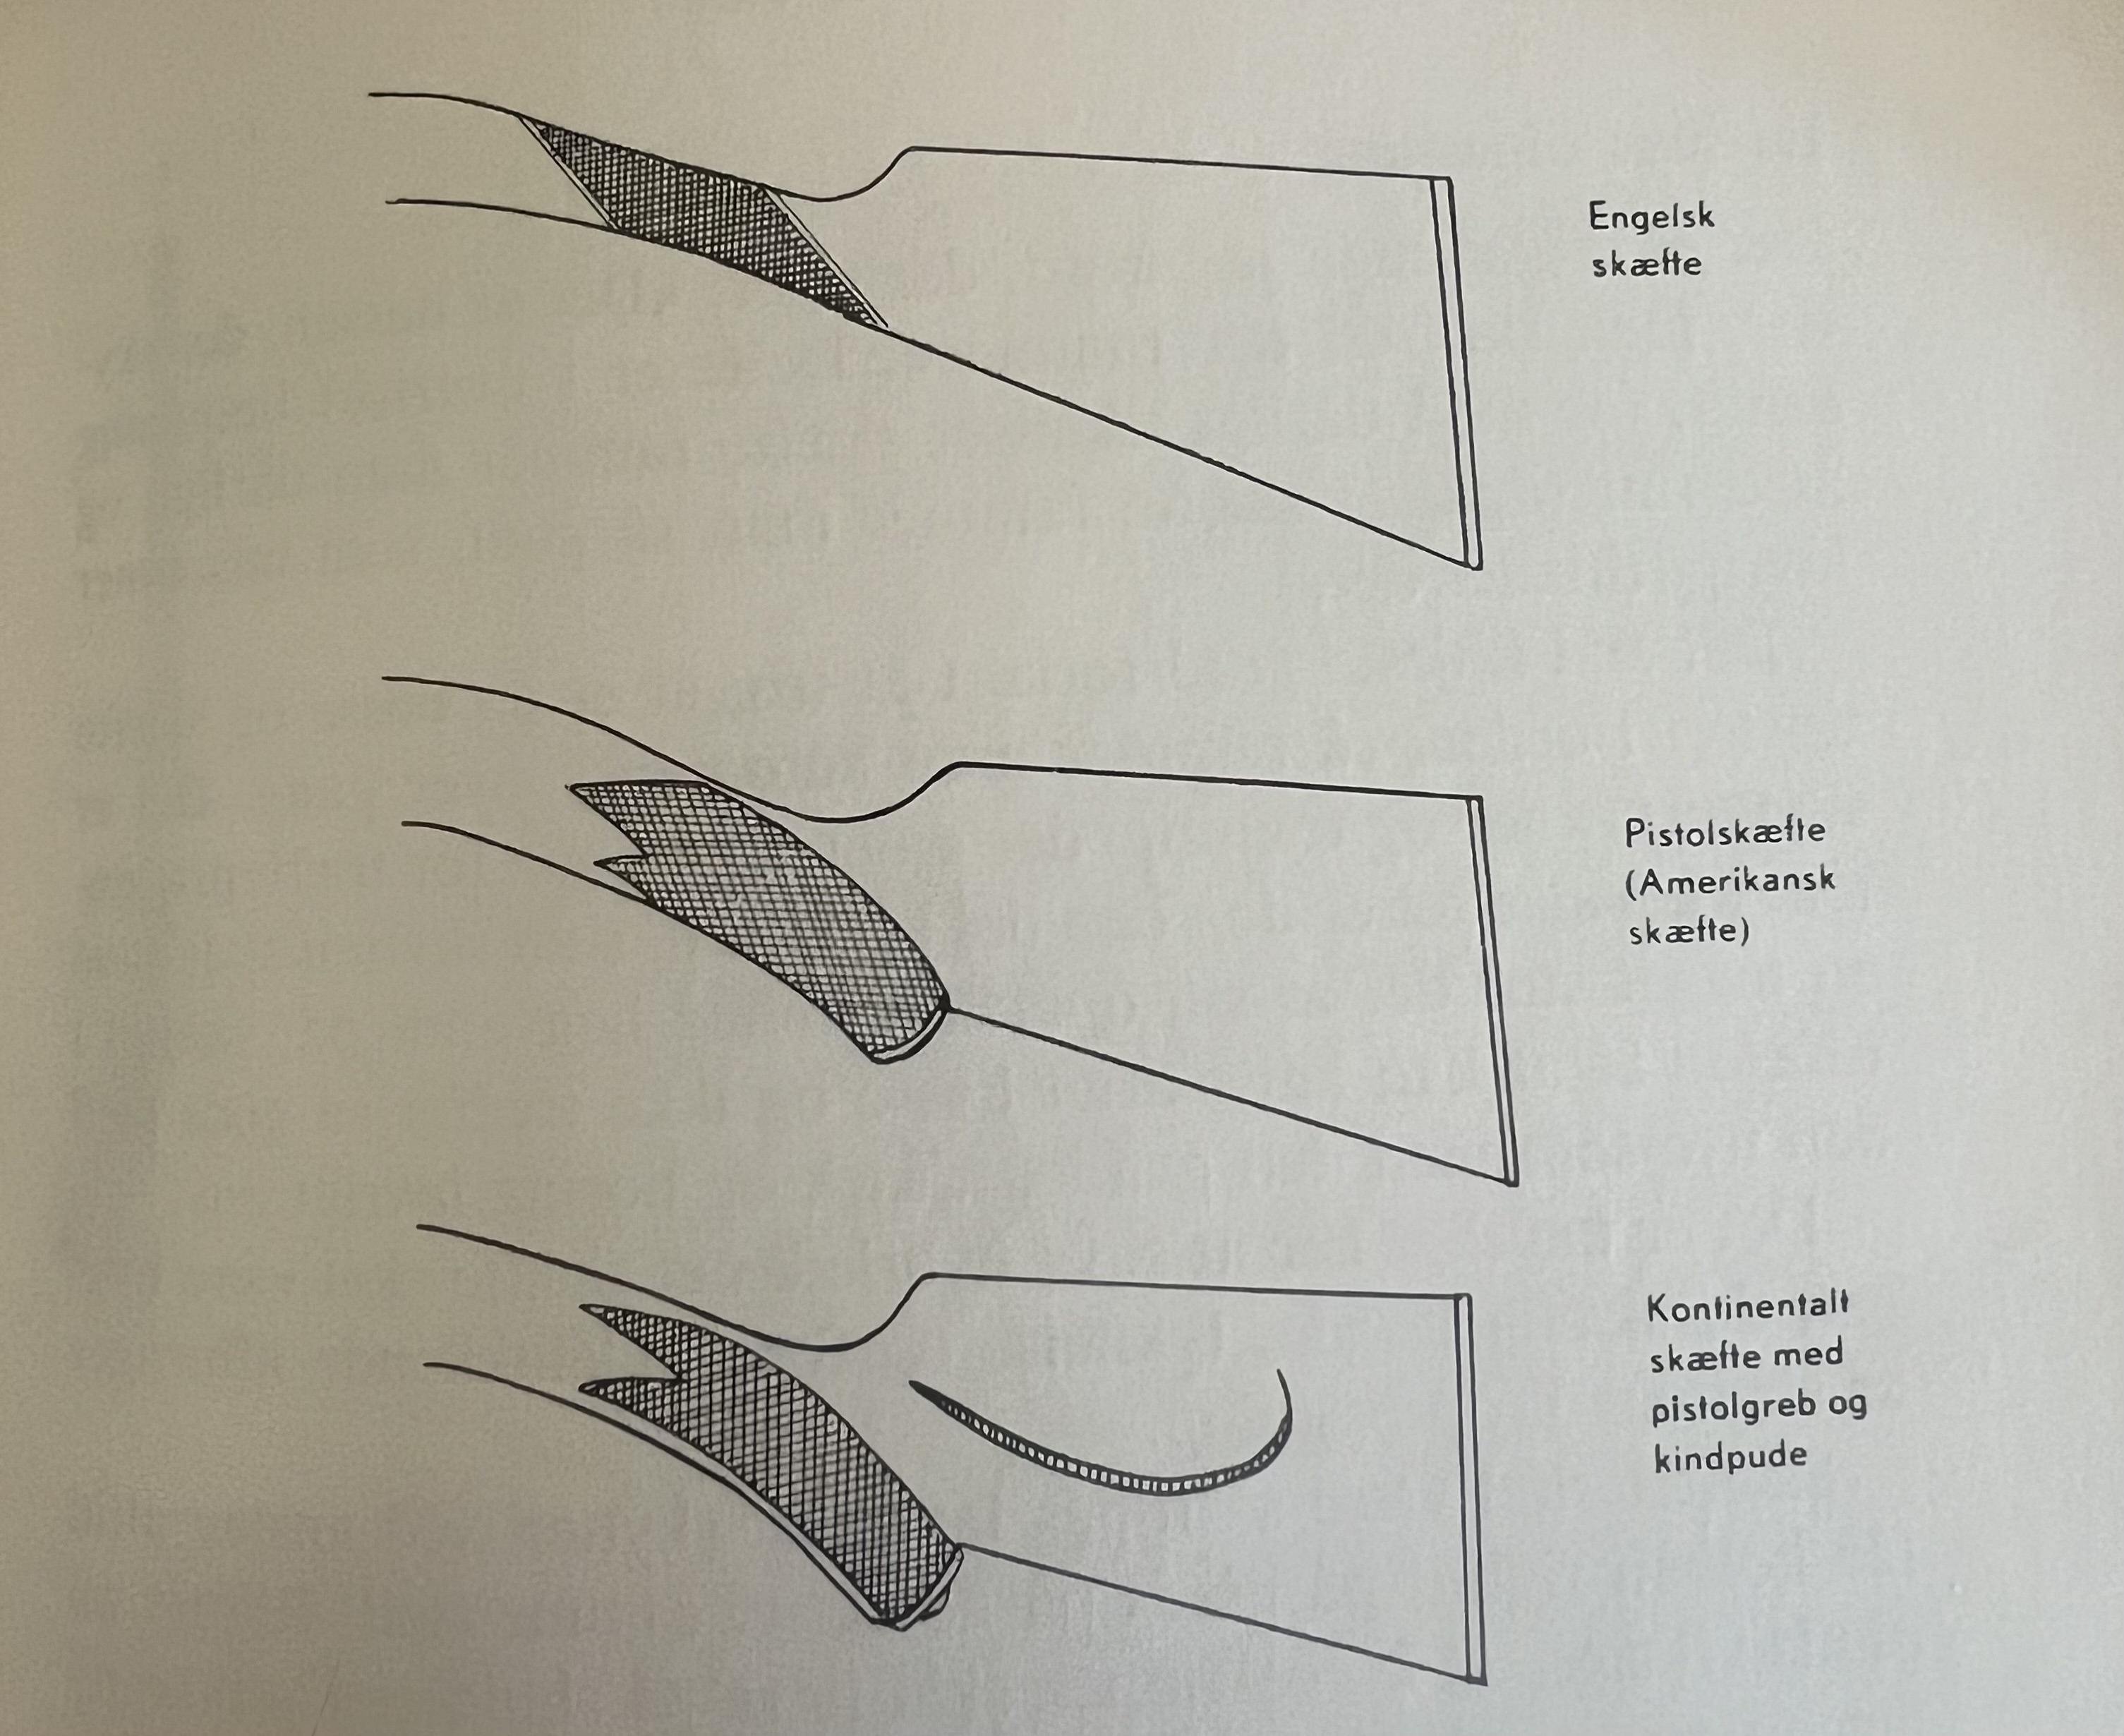
\includegraphics[width=0.5\textwidth]{Billeder/Andet/haglskaefter.jpeg}
        % Eller: [height=0.6\textheight] for højde-baseret skalering
    \end{center}
    
    % Her kan du tilføje tekst under billedet
    \vspace{1em}
    
\end{frame}

\begin{frame}{Haglvåben kalibre}
    \begin{center}
        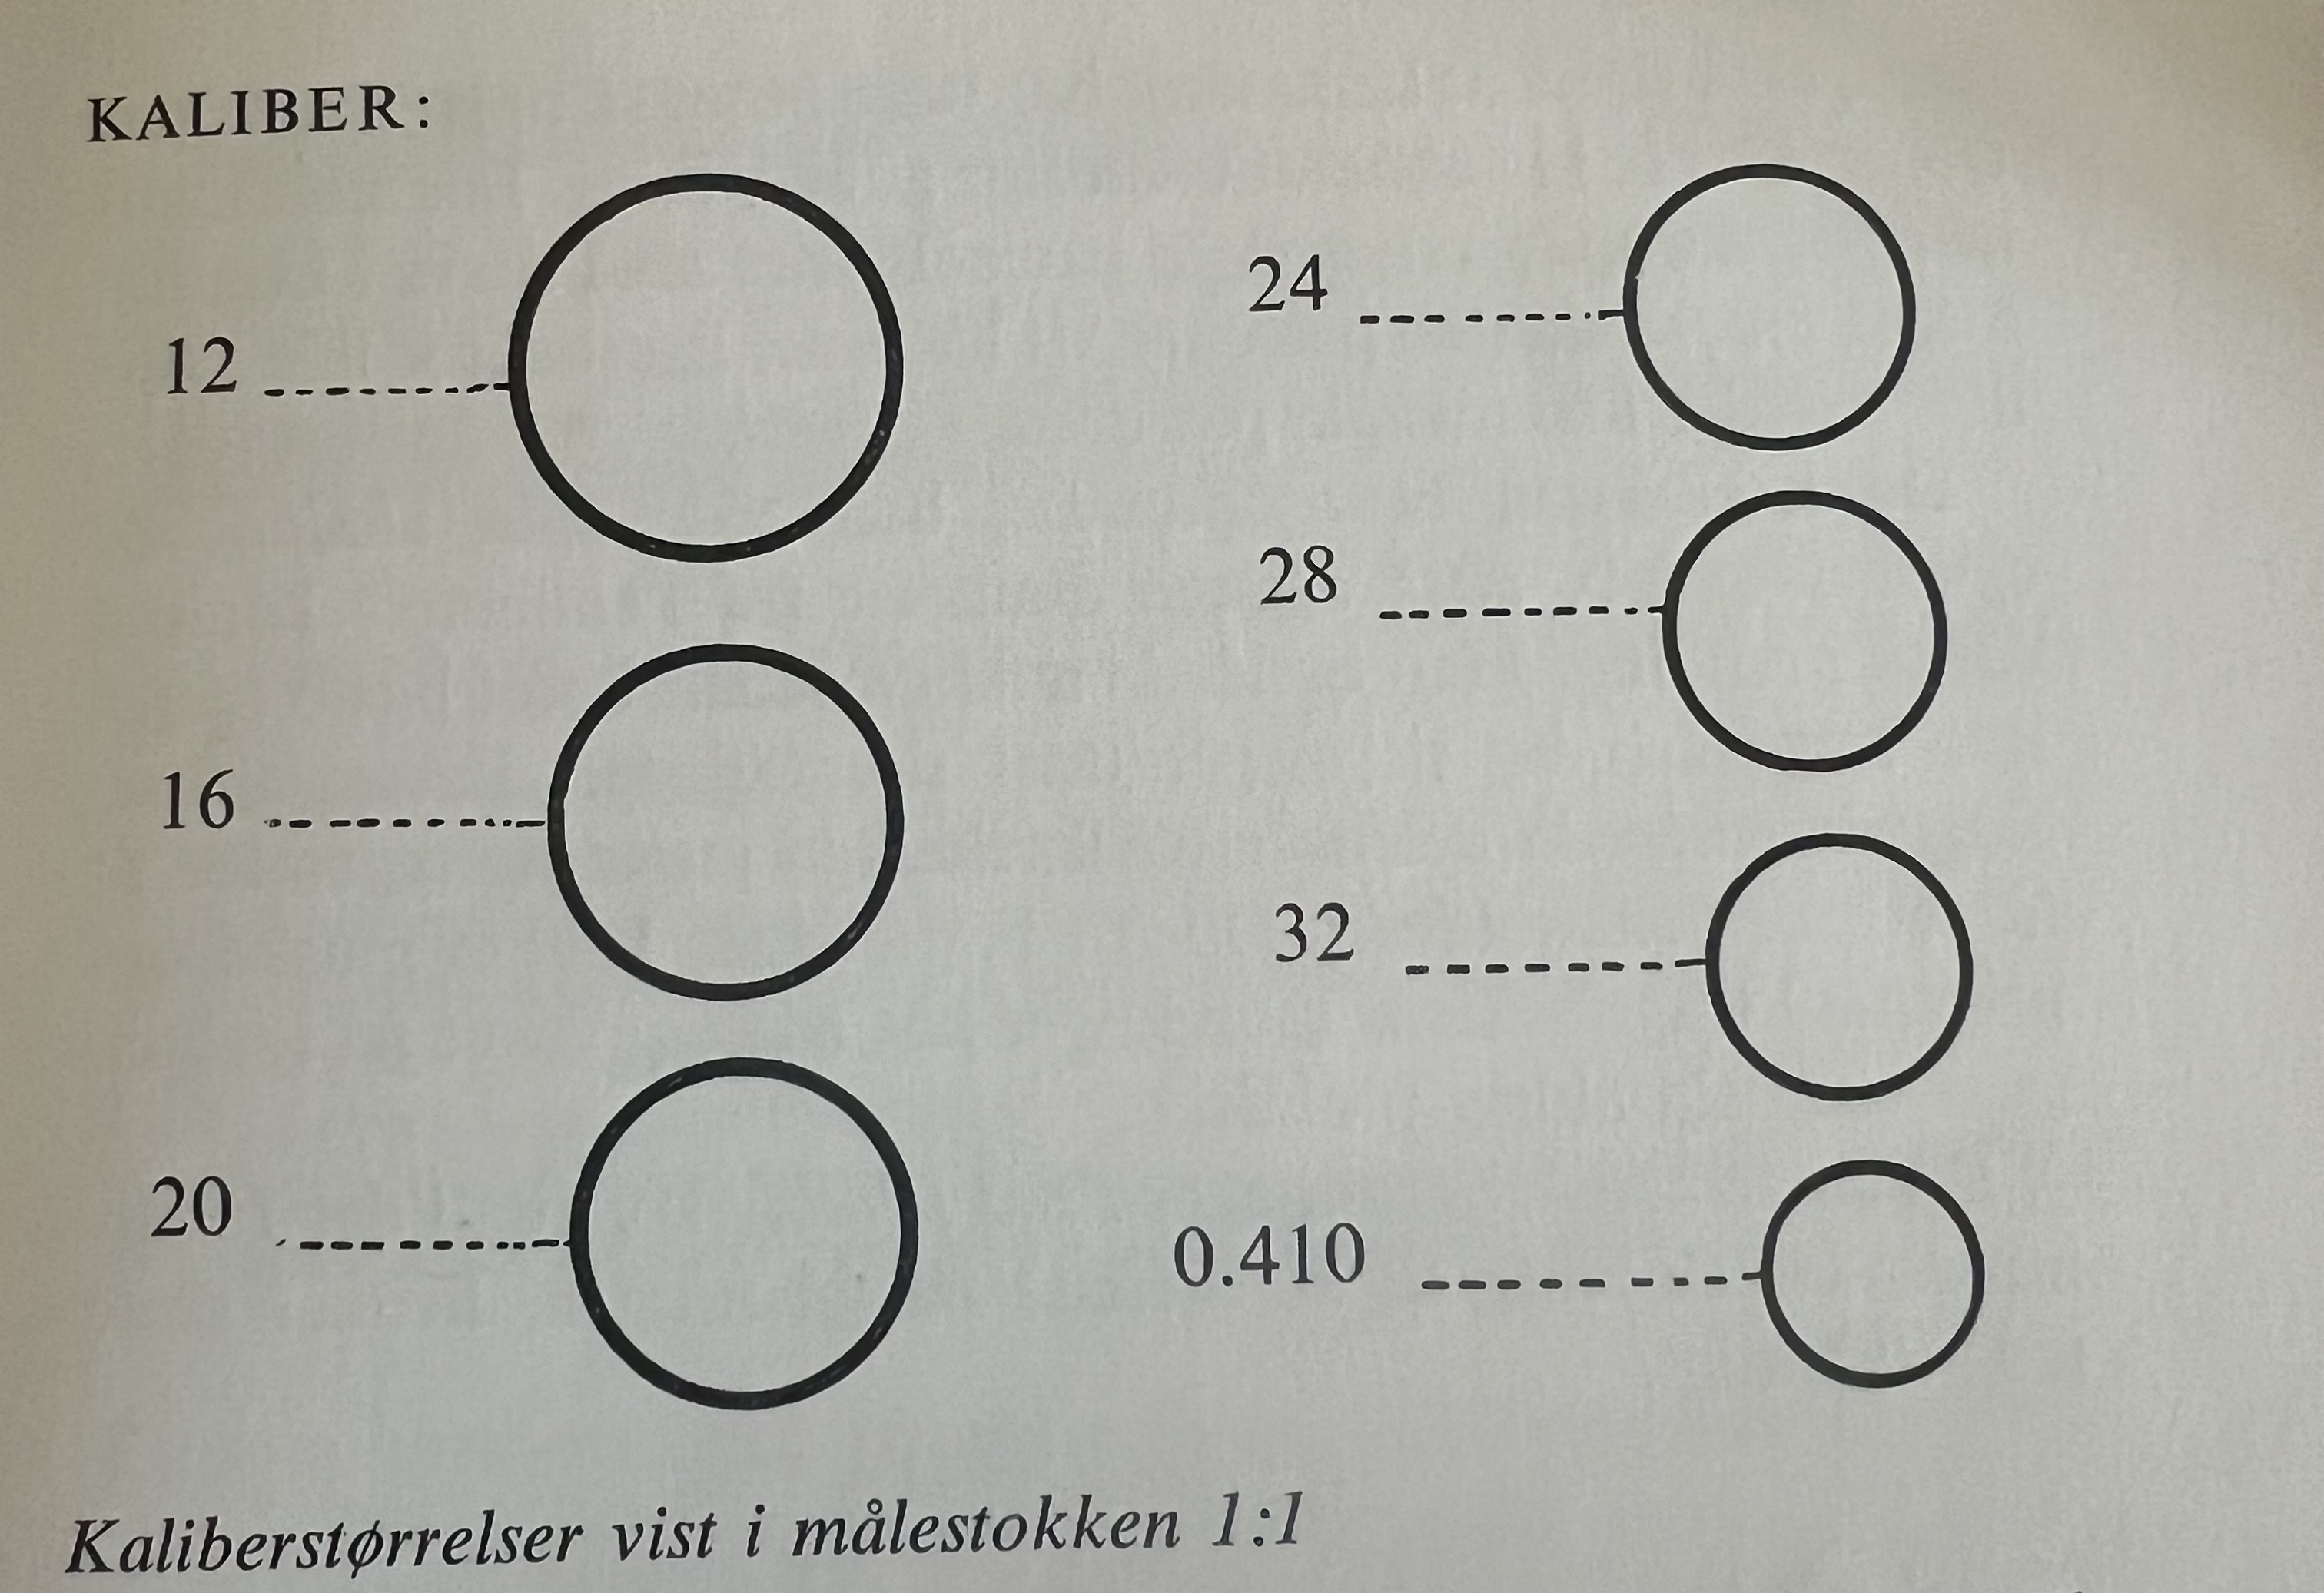
\includegraphics[width=0.5\textwidth]{Billeder/Andet/haglkalibre.jpeg}
        % Eller: [height=0.6\textheight] for højde-baseret skalering
    \end{center}
    
    % Her kan du tilføje tekst under billedet
    \vspace{1em}
    
\end{frame}

\begin{frame}{Sikkerhed med ammunition}
    \begin{itemize}
        \item Forkert kaliber til gevær (tilstopning)
        \item Håndtering af klikker (peg sikker retning, afvrid projektil)
    \end{itemize}
\end{frame}

\begin{frame}{Haglstørrelser og sikkerhedsafstand}
    \begin{center}
        \begin{tabular}{|c|c|c|}
            \hline
            
            \textbf{Nr.} & \textbf{Diameter (mm)} & \textbf{Sikkerhedsafstand (ca. ×100)} \\
            \hline
            Nr. 1 & 4,00 mm & 400 m \\
            Nr. 2 & 3,75 mm & 375 m \\
            Nr. 3 & 3,50 mm & 350 m \\
            Nr. 4 & 3,25 mm & 325 m \\
            Nr. 5 & 3,00 mm & 300 m \\
            Nr. 6 & 2,75 mm & 275 m \\
            Nr. 7 & 2,50 mm & 250 m \\
            \hline
        \end{tabular}
    \end{center}
    
    \vspace{1em}
    \small
    \textbf{Bemærk:} \\
    $\times 100$ er en meget grov tommelfingerregel for potentiel maksimal rækkevidde ved høj affyringsvinkel. \\
    Reelt: Nr. 1–2 hagl kan nå 200–300 m ved flad skud, men op til 400+ m ved stejl vinkel. \\
    Altid hold 200–300 m sikkerhedsafstand til veje, huse, mennesker mv. – uanset haglstørrelse!
\end{frame}

\begin{frame}{Sikkerhedsafstande riffel}
    \begin{itemize}
        \item Alm jagtriffel = 5000 m (5km)
        \item Salonriffel = 3000 m (3km)
    \end{itemize}
\end{frame}


\end{document}